\documentclass[]{book}
\usepackage{lmodern}
\usepackage{amssymb,amsmath}
\usepackage{ifxetex,ifluatex}
\usepackage{fixltx2e} % provides \textsubscript
\ifnum 0\ifxetex 1\fi\ifluatex 1\fi=0 % if pdftex
  \usepackage[T1]{fontenc}
  \usepackage[utf8]{inputenc}
\else % if luatex or xelatex
  \ifxetex
    \usepackage{mathspec}
  \else
    \usepackage{fontspec}
  \fi
  \defaultfontfeatures{Ligatures=TeX,Scale=MatchLowercase}
\fi
% use upquote if available, for straight quotes in verbatim environments
\IfFileExists{upquote.sty}{\usepackage{upquote}}{}
% use microtype if available
\IfFileExists{microtype.sty}{%
\usepackage{microtype}
\UseMicrotypeSet[protrusion]{basicmath} % disable protrusion for tt fonts
}{}
\usepackage{hyperref}
\hypersetup{unicode=true,
            pdftitle={Розеттский камень},
            pdfauthor={Пуассон, фея и три мексиканских негодяя},
            pdfborder={0 0 0},
            breaklinks=true}
\urlstyle{same}  % don't use monospace font for urls
\usepackage{natbib}
\bibliographystyle{apalike}
\usepackage{color}
\usepackage{fancyvrb}
\newcommand{\VerbBar}{|}
\newcommand{\VERB}{\Verb[commandchars=\\\{\}]}
\DefineVerbatimEnvironment{Highlighting}{Verbatim}{commandchars=\\\{\}}
% Add ',fontsize=\small' for more characters per line
\usepackage{framed}
\definecolor{shadecolor}{RGB}{248,248,248}
\newenvironment{Shaded}{\begin{snugshade}}{\end{snugshade}}
\newcommand{\AlertTok}[1]{\textcolor[rgb]{0.94,0.16,0.16}{#1}}
\newcommand{\AnnotationTok}[1]{\textcolor[rgb]{0.56,0.35,0.01}{\textbf{\textit{#1}}}}
\newcommand{\AttributeTok}[1]{\textcolor[rgb]{0.77,0.63,0.00}{#1}}
\newcommand{\BaseNTok}[1]{\textcolor[rgb]{0.00,0.00,0.81}{#1}}
\newcommand{\BuiltInTok}[1]{#1}
\newcommand{\CharTok}[1]{\textcolor[rgb]{0.31,0.60,0.02}{#1}}
\newcommand{\CommentTok}[1]{\textcolor[rgb]{0.56,0.35,0.01}{\textit{#1}}}
\newcommand{\CommentVarTok}[1]{\textcolor[rgb]{0.56,0.35,0.01}{\textbf{\textit{#1}}}}
\newcommand{\ConstantTok}[1]{\textcolor[rgb]{0.00,0.00,0.00}{#1}}
\newcommand{\ControlFlowTok}[1]{\textcolor[rgb]{0.13,0.29,0.53}{\textbf{#1}}}
\newcommand{\DataTypeTok}[1]{\textcolor[rgb]{0.13,0.29,0.53}{#1}}
\newcommand{\DecValTok}[1]{\textcolor[rgb]{0.00,0.00,0.81}{#1}}
\newcommand{\DocumentationTok}[1]{\textcolor[rgb]{0.56,0.35,0.01}{\textbf{\textit{#1}}}}
\newcommand{\ErrorTok}[1]{\textcolor[rgb]{0.64,0.00,0.00}{\textbf{#1}}}
\newcommand{\ExtensionTok}[1]{#1}
\newcommand{\FloatTok}[1]{\textcolor[rgb]{0.00,0.00,0.81}{#1}}
\newcommand{\FunctionTok}[1]{\textcolor[rgb]{0.00,0.00,0.00}{#1}}
\newcommand{\ImportTok}[1]{#1}
\newcommand{\InformationTok}[1]{\textcolor[rgb]{0.56,0.35,0.01}{\textbf{\textit{#1}}}}
\newcommand{\KeywordTok}[1]{\textcolor[rgb]{0.13,0.29,0.53}{\textbf{#1}}}
\newcommand{\NormalTok}[1]{#1}
\newcommand{\OperatorTok}[1]{\textcolor[rgb]{0.81,0.36,0.00}{\textbf{#1}}}
\newcommand{\OtherTok}[1]{\textcolor[rgb]{0.56,0.35,0.01}{#1}}
\newcommand{\PreprocessorTok}[1]{\textcolor[rgb]{0.56,0.35,0.01}{\textit{#1}}}
\newcommand{\RegionMarkerTok}[1]{#1}
\newcommand{\SpecialCharTok}[1]{\textcolor[rgb]{0.00,0.00,0.00}{#1}}
\newcommand{\SpecialStringTok}[1]{\textcolor[rgb]{0.31,0.60,0.02}{#1}}
\newcommand{\StringTok}[1]{\textcolor[rgb]{0.31,0.60,0.02}{#1}}
\newcommand{\VariableTok}[1]{\textcolor[rgb]{0.00,0.00,0.00}{#1}}
\newcommand{\VerbatimStringTok}[1]{\textcolor[rgb]{0.31,0.60,0.02}{#1}}
\newcommand{\WarningTok}[1]{\textcolor[rgb]{0.56,0.35,0.01}{\textbf{\textit{#1}}}}
\usepackage{longtable,booktabs}
\usepackage{graphicx,grffile}
\makeatletter
\def\maxwidth{\ifdim\Gin@nat@width>\linewidth\linewidth\else\Gin@nat@width\fi}
\def\maxheight{\ifdim\Gin@nat@height>\textheight\textheight\else\Gin@nat@height\fi}
\makeatother
% Scale images if necessary, so that they will not overflow the page
% margins by default, and it is still possible to overwrite the defaults
% using explicit options in \includegraphics[width, height, ...]{}
\setkeys{Gin}{width=\maxwidth,height=\maxheight,keepaspectratio}
\IfFileExists{parskip.sty}{%
\usepackage{parskip}
}{% else
\setlength{\parindent}{0pt}
\setlength{\parskip}{6pt plus 2pt minus 1pt}
}
\setlength{\emergencystretch}{3em}  % prevent overfull lines
\providecommand{\tightlist}{%
  \setlength{\itemsep}{0pt}\setlength{\parskip}{0pt}}
\setcounter{secnumdepth}{5}
% Redefines (sub)paragraphs to behave more like sections
\ifx\paragraph\undefined\else
\let\oldparagraph\paragraph
\renewcommand{\paragraph}[1]{\oldparagraph{#1}\mbox{}}
\fi
\ifx\subparagraph\undefined\else
\let\oldsubparagraph\subparagraph
\renewcommand{\subparagraph}[1]{\oldsubparagraph{#1}\mbox{}}
\fi

%%% Use protect on footnotes to avoid problems with footnotes in titles
\let\rmarkdownfootnote\footnote%
\def\footnote{\protect\rmarkdownfootnote}

%%% Change title format to be more compact
\usepackage{titling}

% Create subtitle command for use in maketitle
\providecommand{\subtitle}[1]{
  \posttitle{
    \begin{center}\large#1\end{center}
    }
}

\setlength{\droptitle}{-2em}

  \title{Розеттский камень}
    \pretitle{\vspace{\droptitle}\centering\huge}
  \posttitle{\par}
    \author{Пуассон, фея и три мексиканских негодяя}
    \preauthor{\centering\large\emph}
  \postauthor{\par}
      \predate{\centering\large\emph}
  \postdate{\par}
    \date{2019-09-22}

\usepackage{booktabs} % красивые таблицы
\usepackage{polyglossia} % переключение языков в xelatex
\setmainlanguage{russian} 
\newfontfamily{\cyrillicfont}{Linux Libertine O} % залатываем какой-то косяк с русскими шрифтами
\newfontfamily{\cyrillicfonttt}{Linux Libertine O}

\begin{document}
\maketitle

{
\setcounter{tocdepth}{1}
\tableofcontents
}
\hypertarget{-}{%
\chapter{Напутственное слово}\label{-}}

\hypertarget{installsoft}{%
\chapter{Коан об установке софта}\label{installsoft}}

В этом коане мы рассмотрим установку и настройку программ для работы на языках программирования R и Python, а также установку и настройку программы Stata.

\begin{center}\rule{0.5\linewidth}{\linethickness}\end{center}

\#\#\#Язык программирования R
\textgreater{} R - это открытая среда программирования, помогающая в работе со статистическими данными. Для программирования на R подойдет программа RStudio.

Рассмотрим установку RStudio на Mac OS и Windows.

\#\#\#\#\#Инструкция по установке RStudio для Windows / Mac OS:

\begin{enumerate}
\def\labelenumi{\arabic{enumi}.}
\tightlist
\item
  Загрузите и установите язык программирования R \href{http://cran.cnr.berkeley.edu/}{с официального сайта}.
\end{enumerate}

\begin{itemize}
\item
  Версия для Windows: Выберите ``Download R for Windows'' ▶ ``base'' ▶ ``Download R 3.x.x for Windows''.
\item
  Версия для Mac OS: Выберите ``Download R for (Mac) OS X'' ▶ ``Latest Release'' ▶ ``R 3.x.x''.
\end{itemize}

\begin{enumerate}
\def\labelenumi{\arabic{enumi}.}
\setcounter{enumi}{1}
\tightlist
\item
  Загрузите программу RStudio \href{https://www.rstudio.com/products/rstudio/download/}{с официального сайта разработчика} (выберите подходящую версию из предложенных опций). Возможностей бесплатной версии
  будет вполне достаточно для работы.
  
\includegraphics{images/RStudio.png}
\end{enumerate}

Готово, Вы можете использовать RStudio на вашем компьютере.

\#\#\#\#\#Начало работы

\begin{figure}
\centering
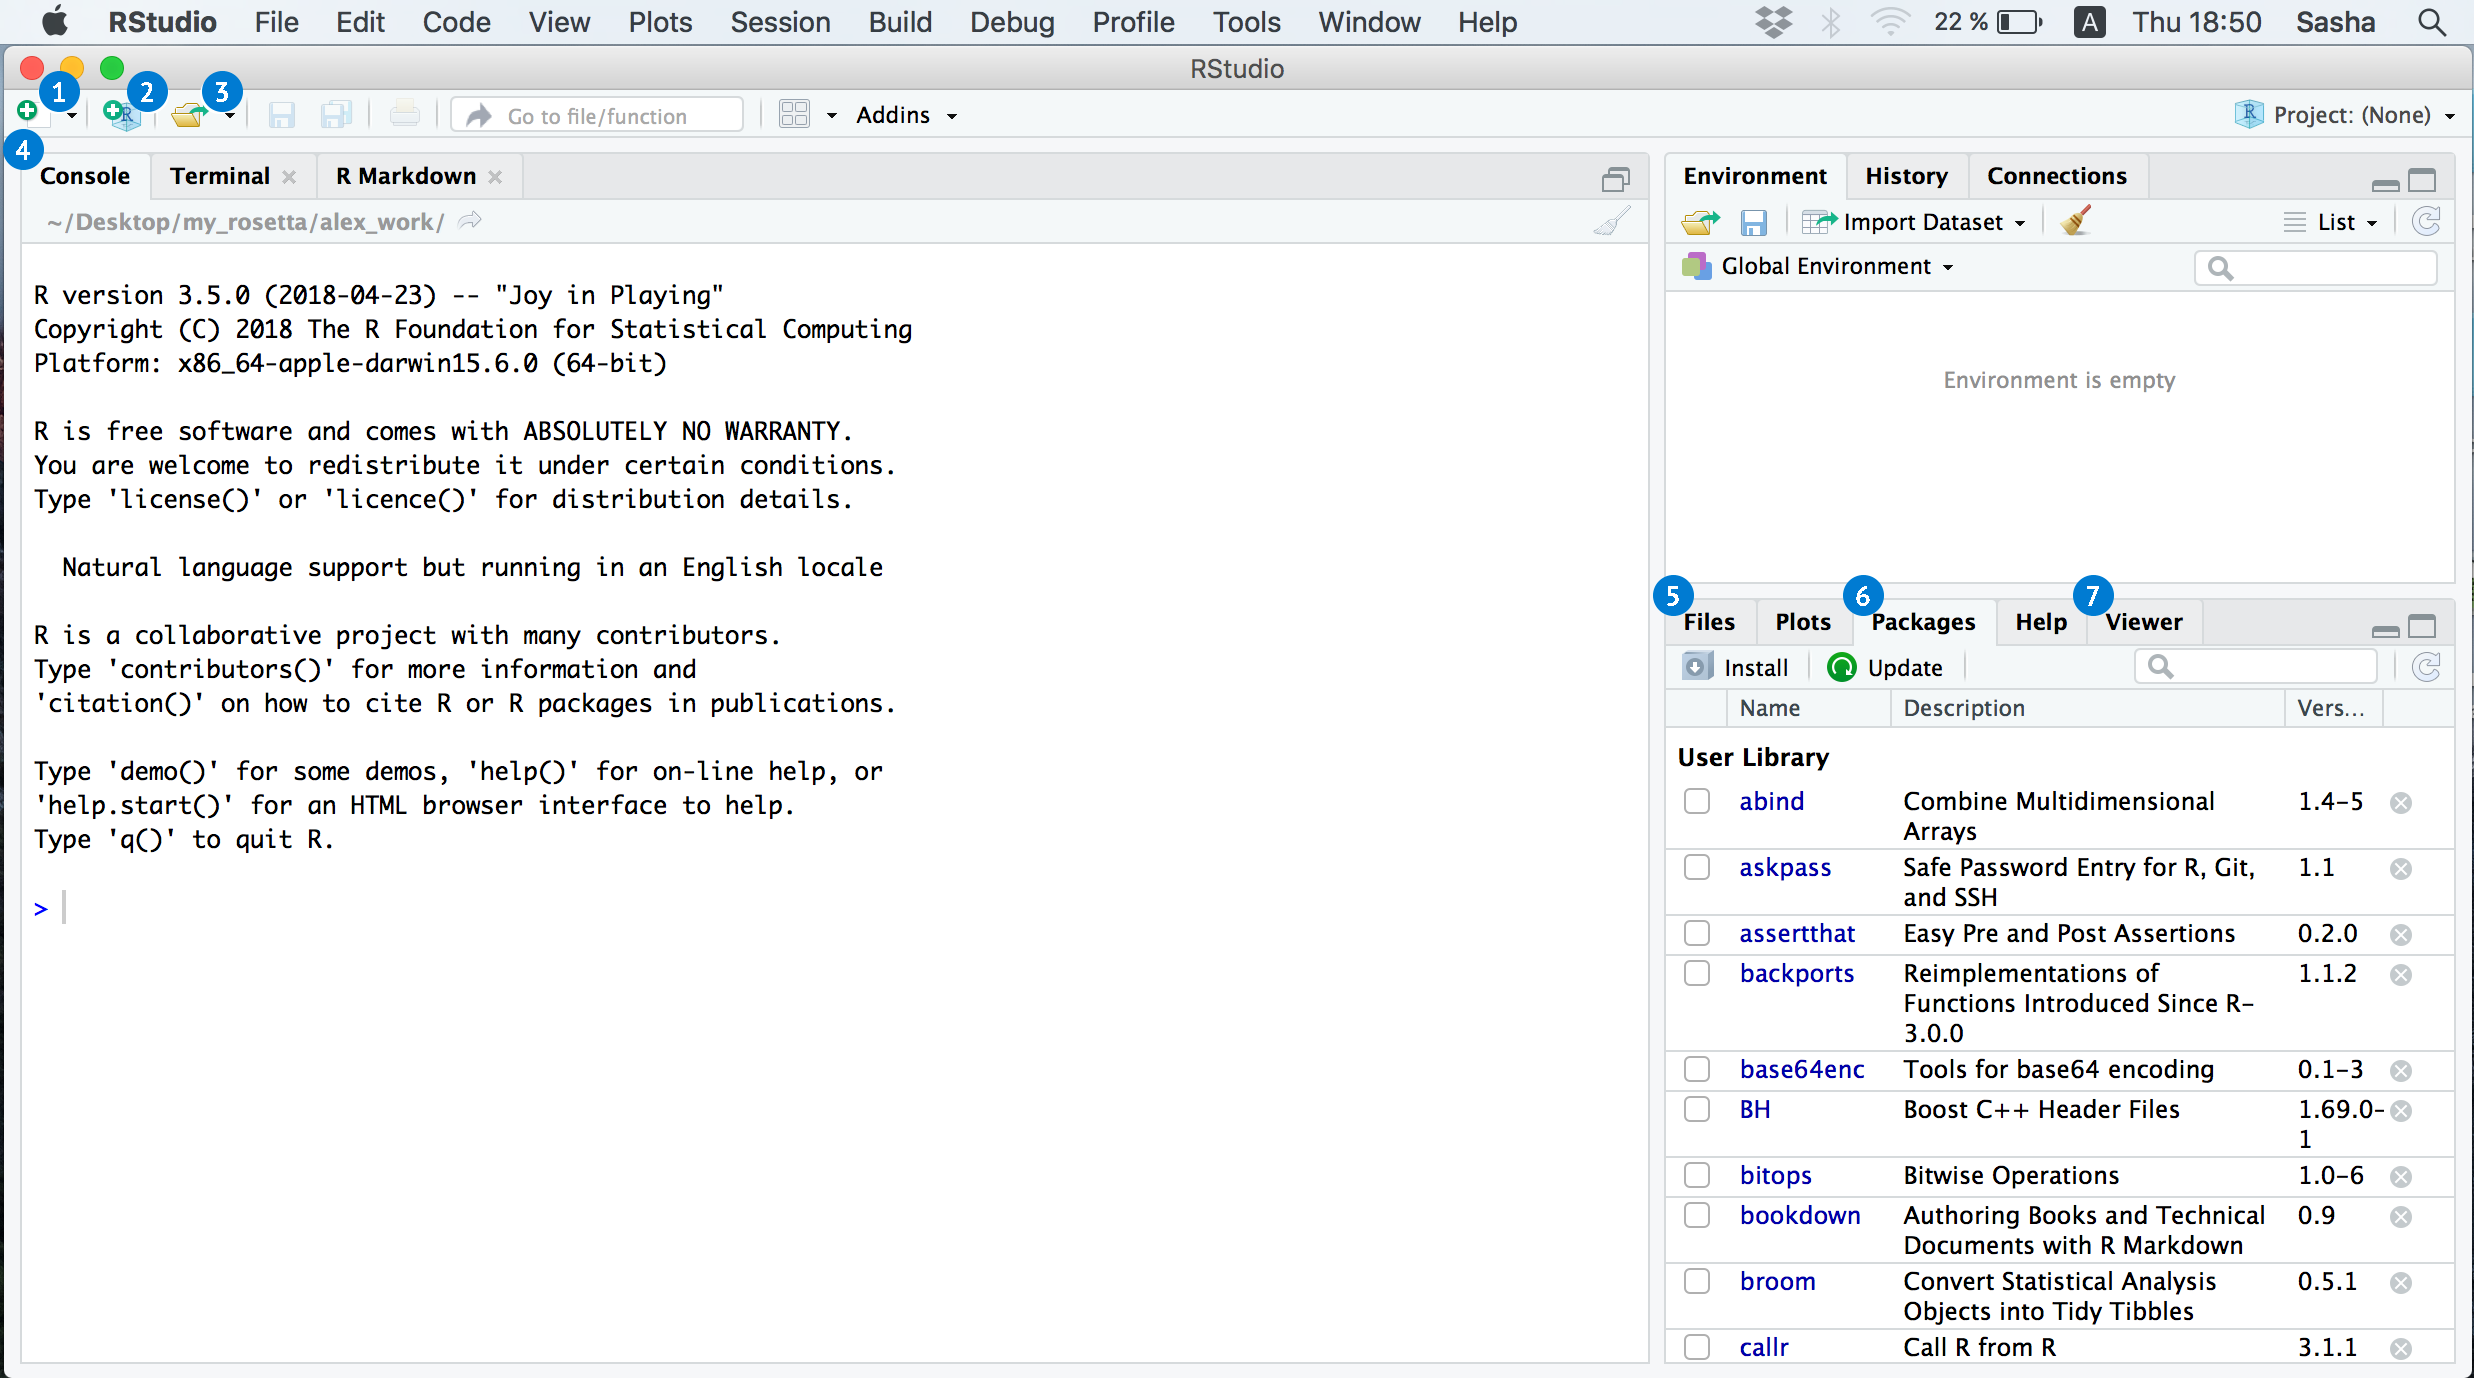
\includegraphics{images/RStudio_Interface.png}
\caption{\emph{Интерфейс программы}}
\end{figure}

\begin{enumerate}
\def\labelenumi{\arabic{enumi}.}
\item
  \textbf{New file} - Создание нового файла.
\item
  \textbf{New project} - Создание нового проекта.
\item
  \textbf{Open file} - Открытие существующего файла.
\item
  \textbf{Console} - Консоль, в которой набирается код.
\item
  \textbf{Files} - Список файлов, доступных для работы.
\item
  \textbf{Packages} - Список установленных пакетов, т.е. расширений. Также можно ознакомиться с ним, введя в консоль команду \emph{installed.packages()}.
\item
  \textbf{Viewer} - Отображение введенного кода.
\end{enumerate}

\begin{center}\rule{0.5\linewidth}{\linethickness}\end{center}

\#\#\#Язык программирования Python
\textgreater{} Python - это ещё одна открытая среда программирования, помогающая в работе со статистическими данными. Для программирования на Python подойдет программа Jupyter Notebook.

\#\#\#\#\#Установка

\begin{enumerate}
\def\labelenumi{\arabic{enumi}.}
\item
  Загрузите и установите Anaconda \href{https://www.anaconda.com/distribution/}{с официального сайта}.
\item
  После загрузки и установки откройте Anaconda Navigator, через который Вы сможете открыть программу Jupyter Notebook.
  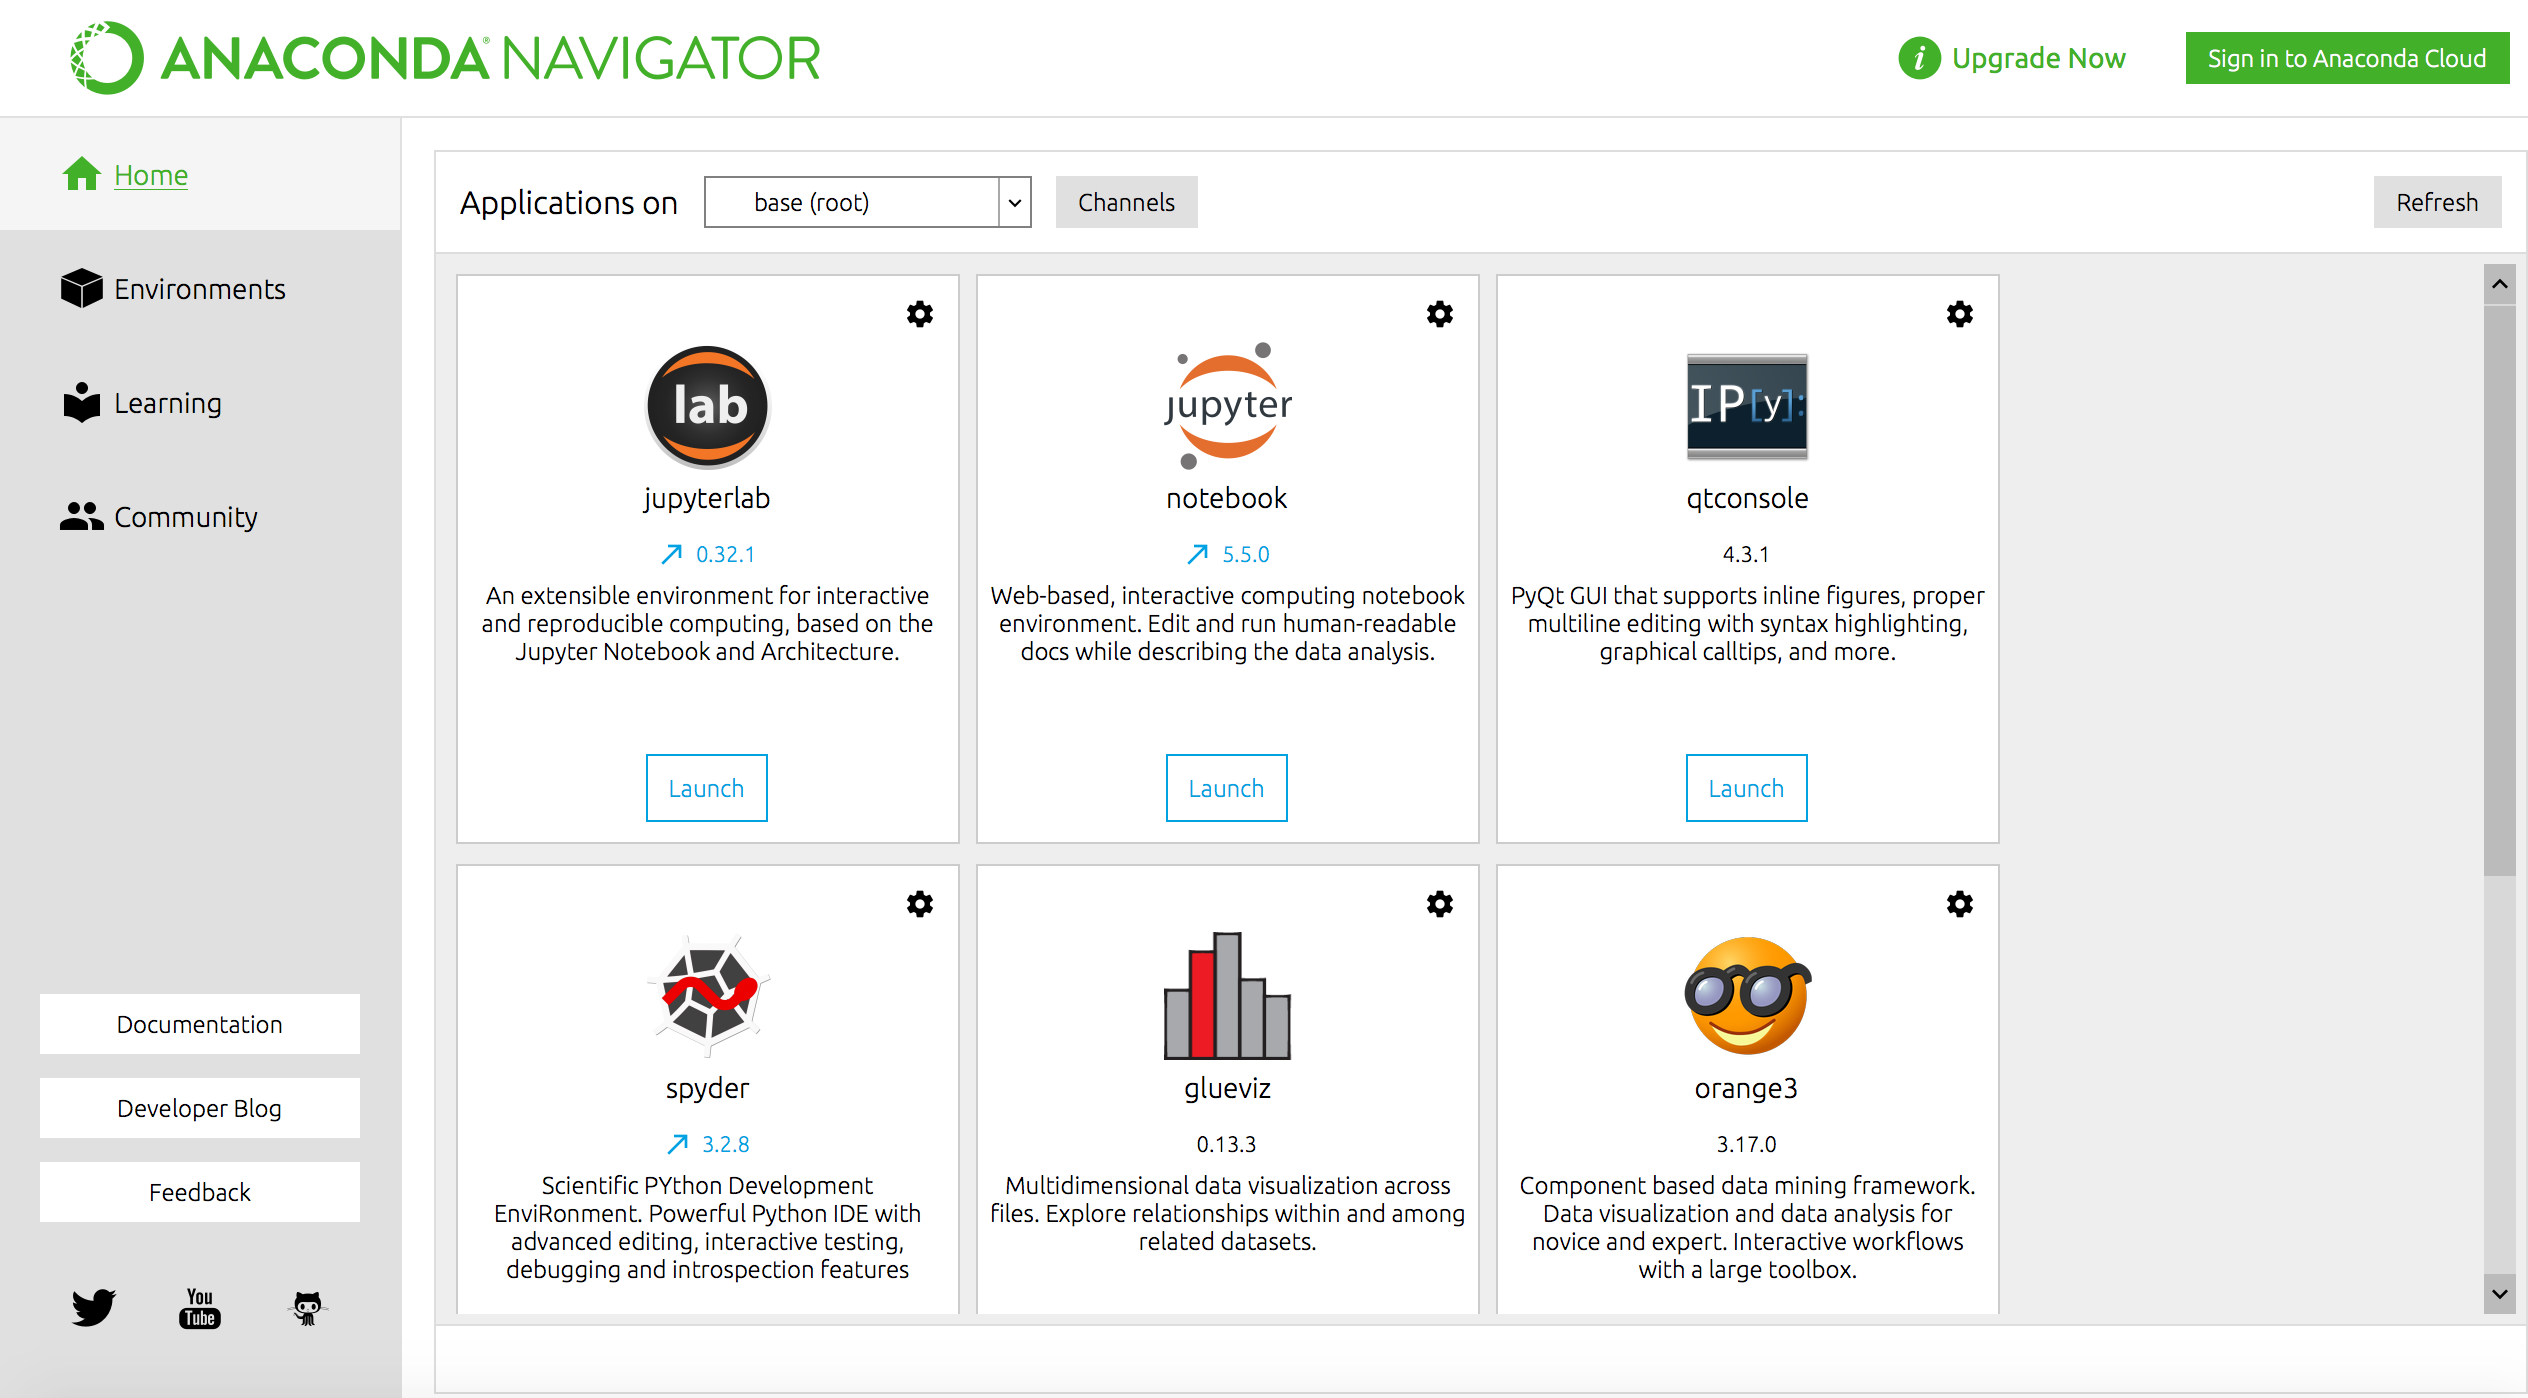
\includegraphics{images/Anaconda Navigator.png}
\end{enumerate}

\#\#\#\#\#Начало работы

Открыв Jupyter Notebook, вы попадете на страницу, содержащую ваши сохраненные файлы. Чтобы создать новый файл, нажмите ``New'' ▶ ``Notebook: Python 3''.
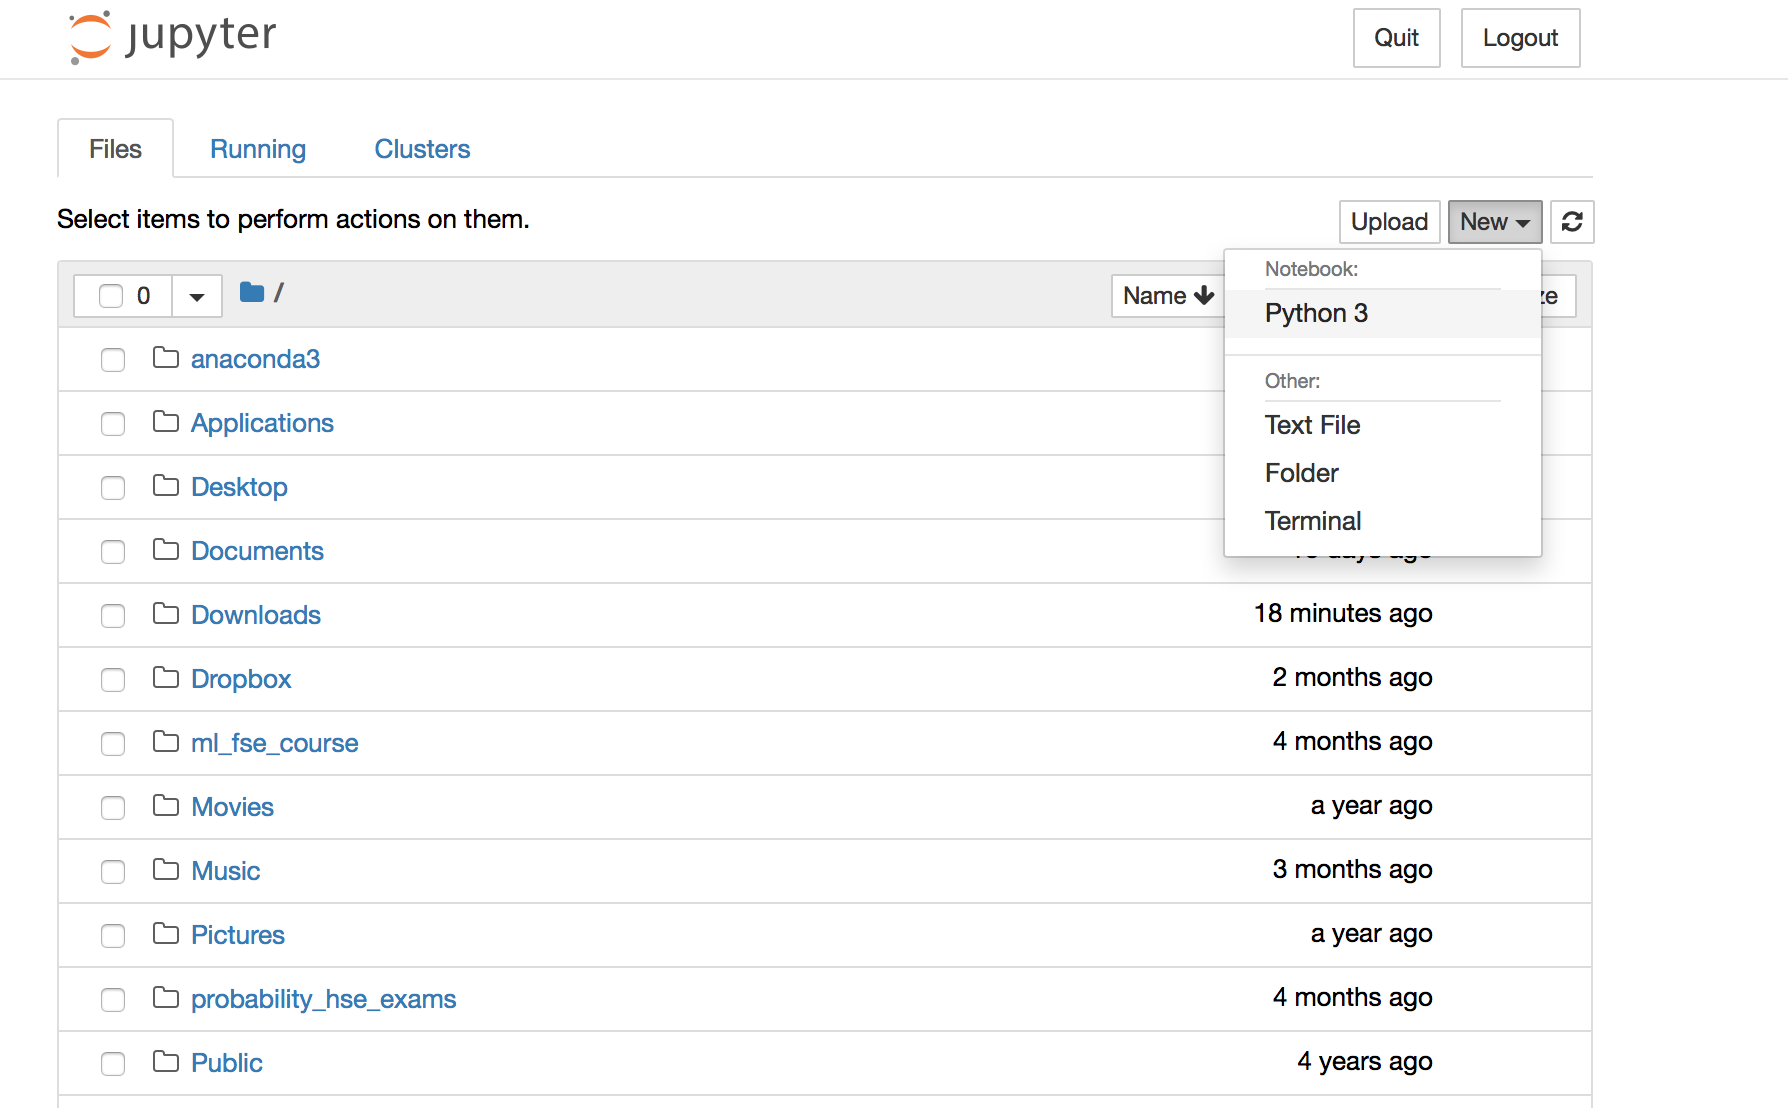
\includegraphics{images/New File in Jupyter.png}

Затем, в открывшемся окне, появится новый файл. Теперь все готово к работе. Вы можете вводить свой код и затем, используя комбинацию клавиш ``Shift'' + ``Enter'', проверять его исполнение.
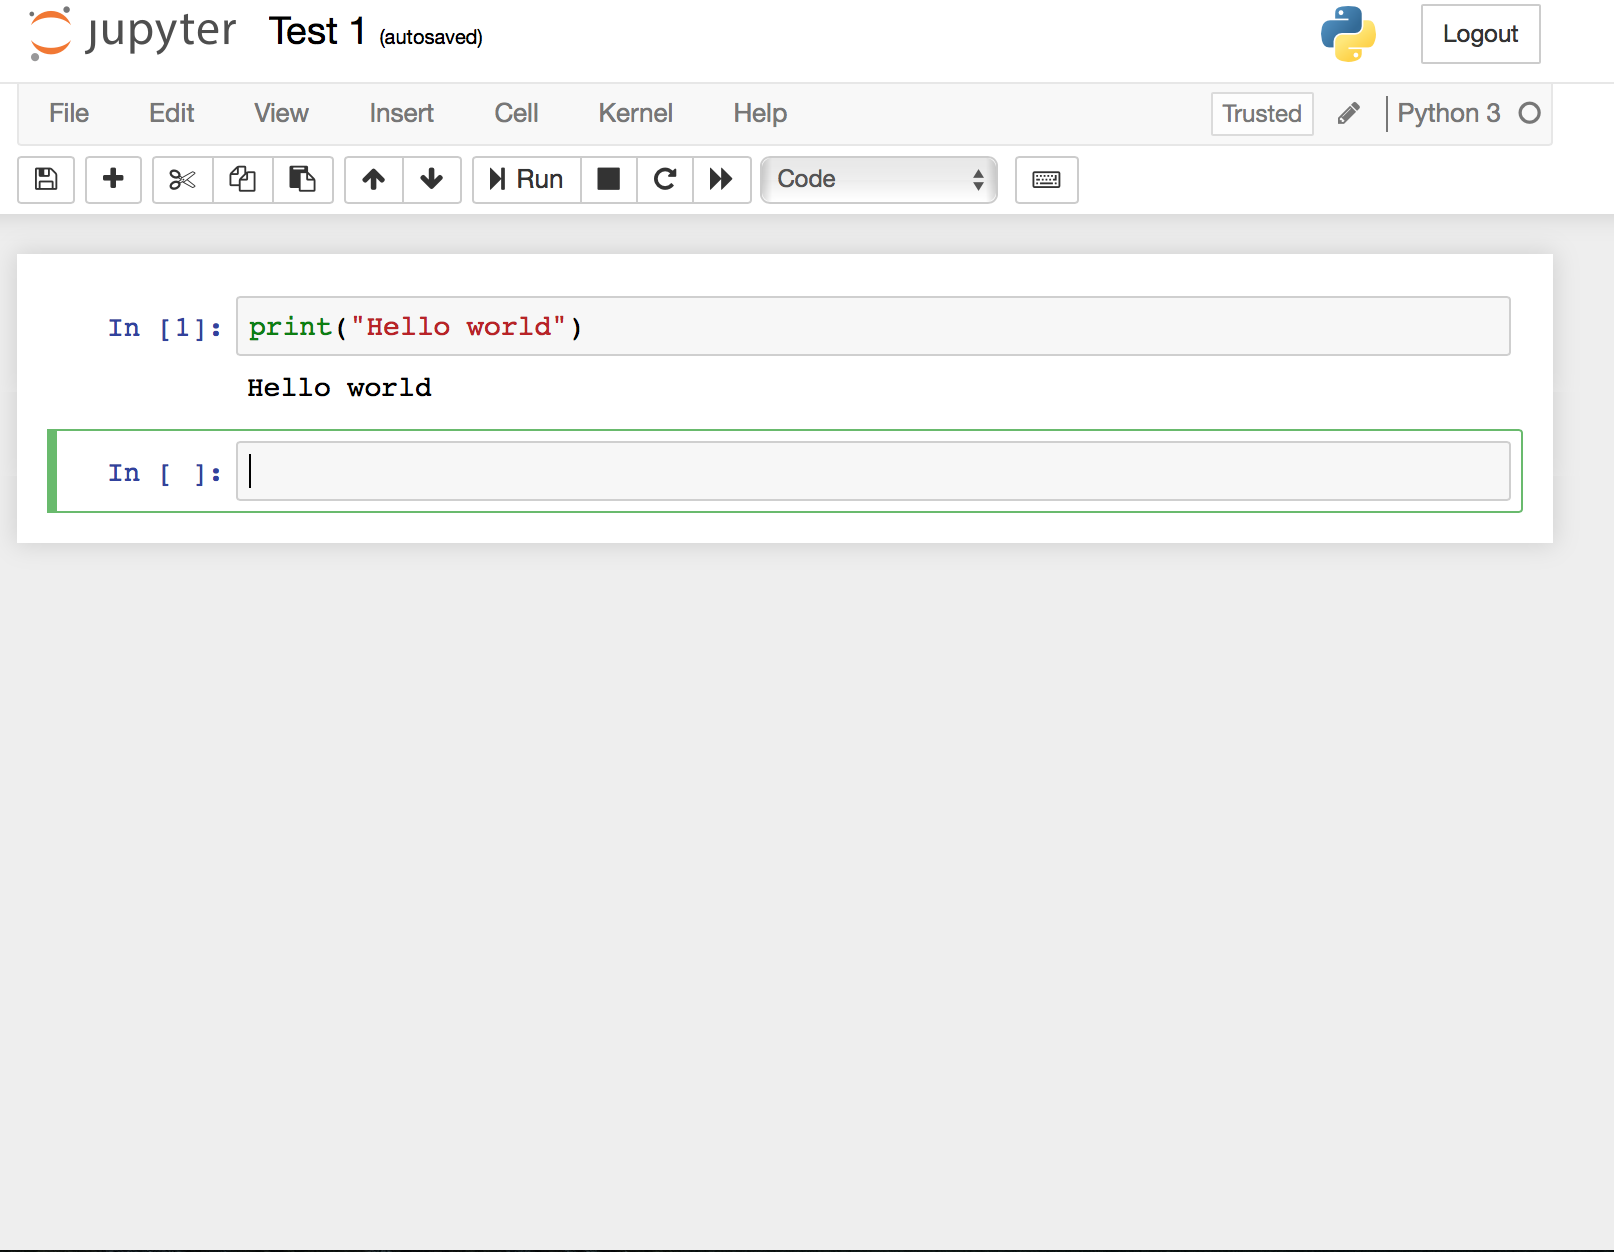
\includegraphics{images/Code in Jupyter.png}

\begin{center}\rule{0.5\linewidth}{\linethickness}\end{center}

\#\#\#Программа STATA
\textgreater{} Stata, в отличие от R и Python, является программой, а не языком программирования. Она также помогает в работе со статистическими данными.

\#\#\#\#\#Установка:

Для установки Stata необходимо загрузить актуальную версию \href{https://www.stata.com/}{с сайта компании-разработчика}. Подойдут как Stata SE, так и Stata MP.

\#\#\#\#\#Начало работы:

\begin{figure}
\centering
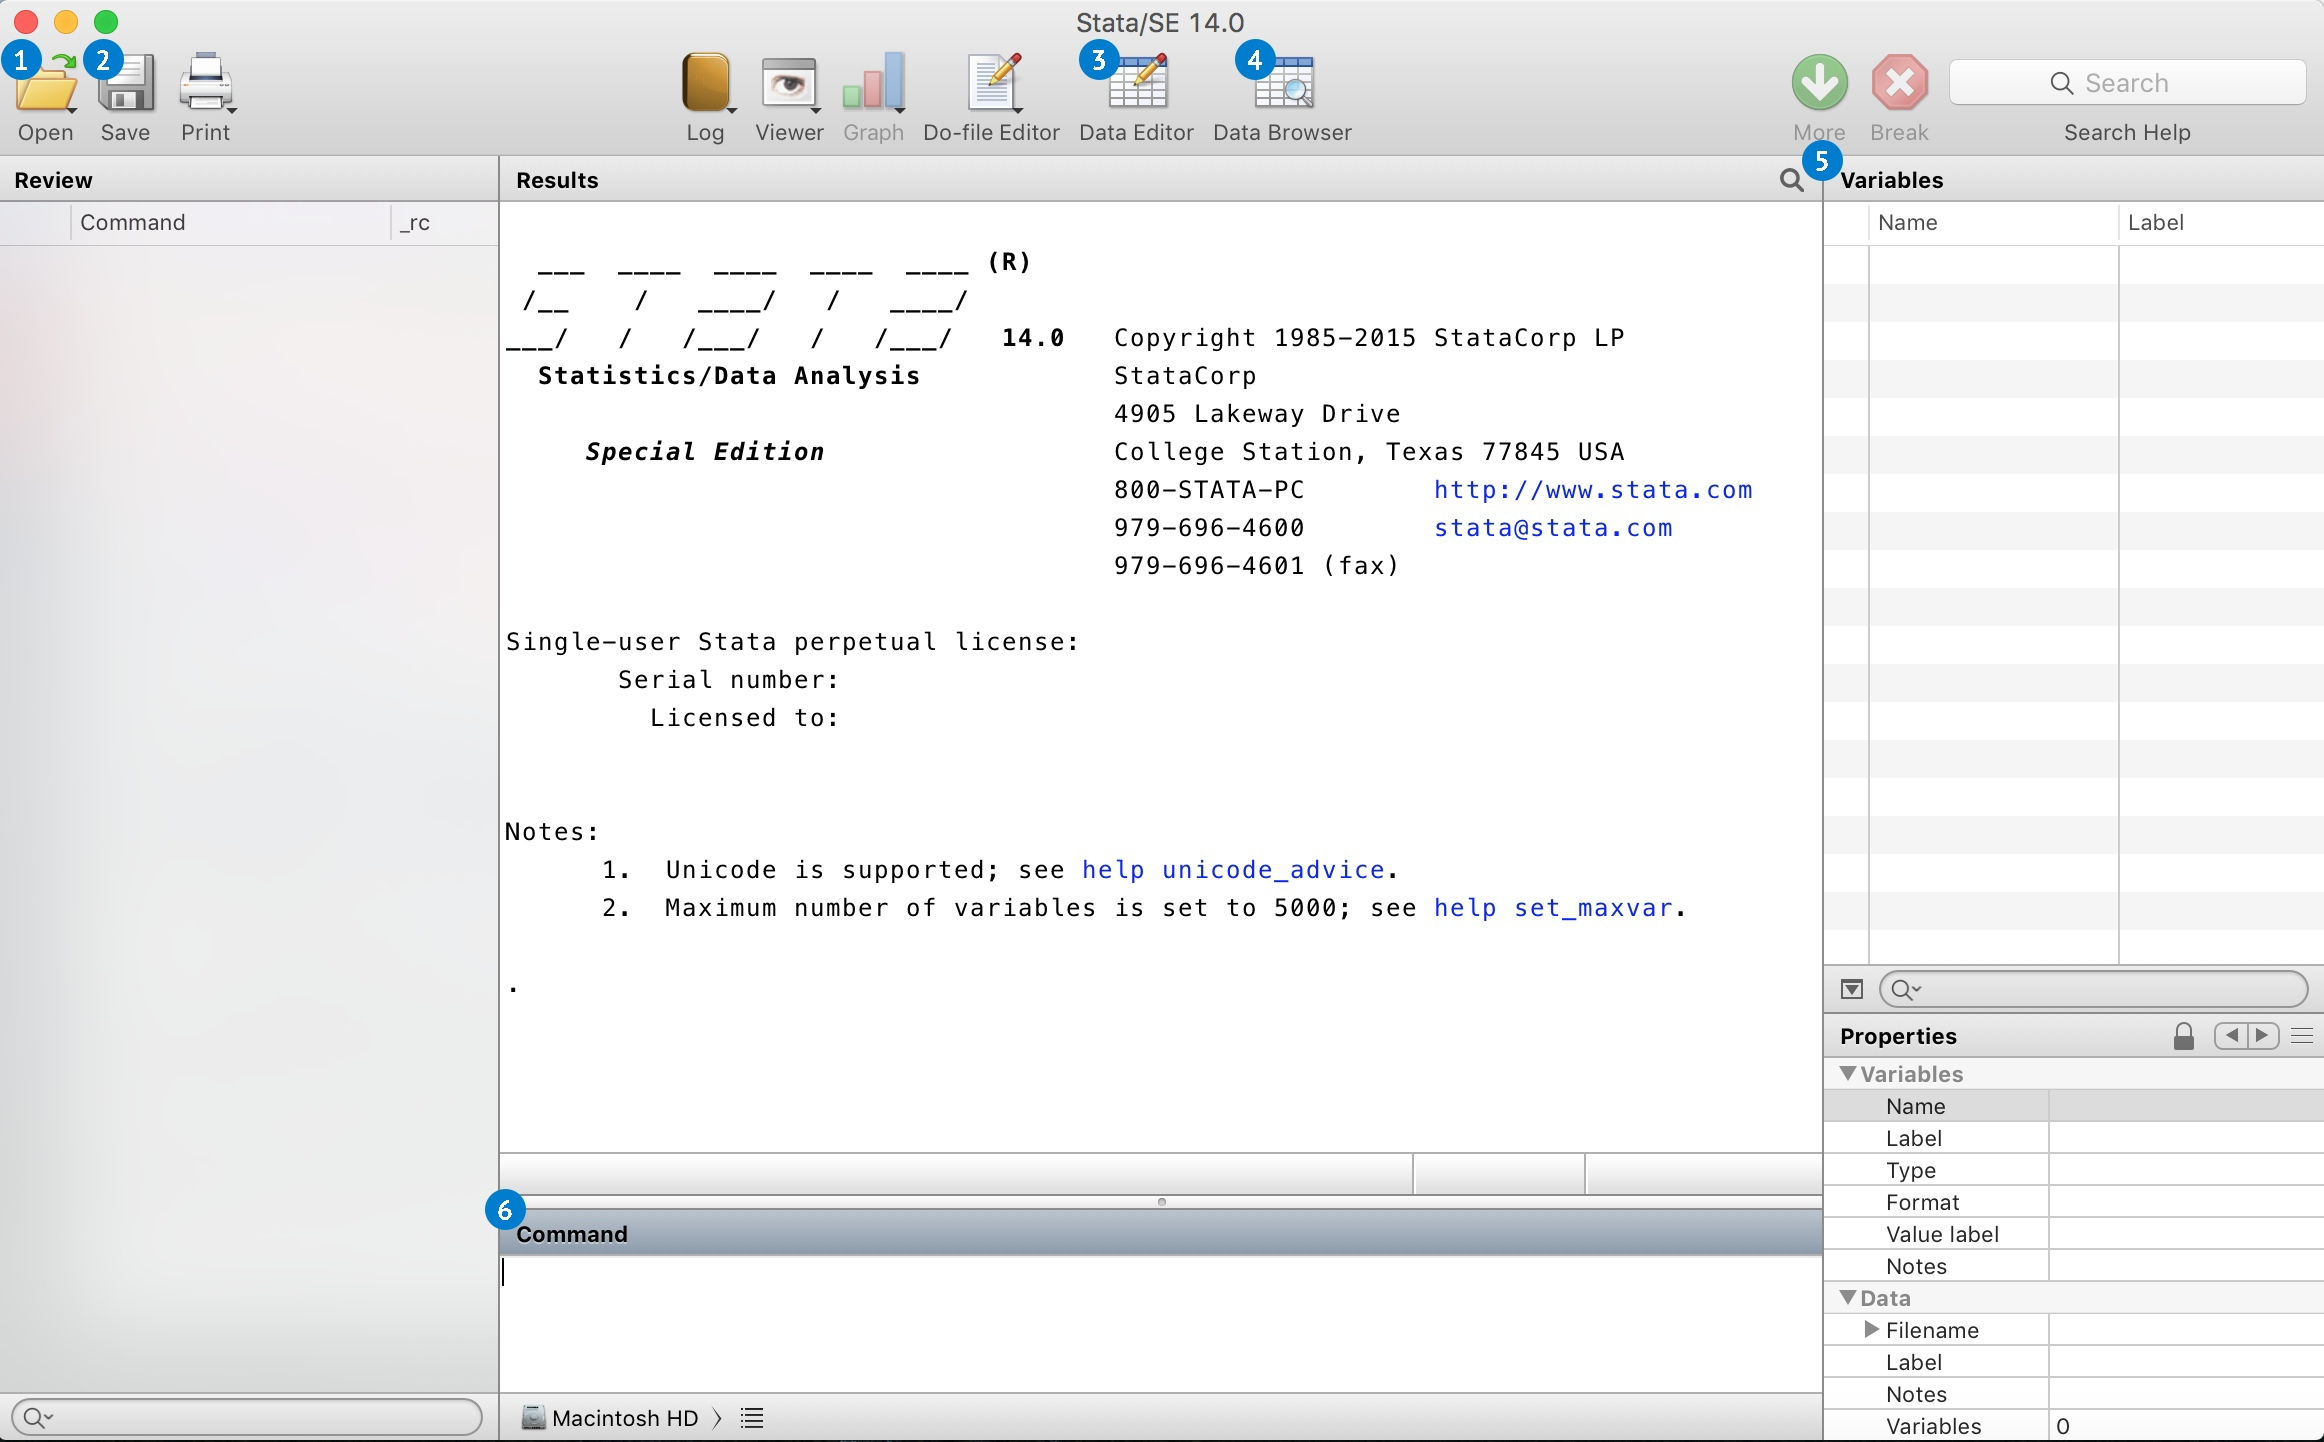
\includegraphics{images/Stata Interface.jpg}
\caption{\emph{Интерфейс Stata}}
\end{figure}

\begin{enumerate}
\def\labelenumi{\arabic{enumi}.}
\tightlist
\item
  \textbf{Open File} - открыть файл.
\item
  \textbf{Save} - сохранить файл.
\item
  \textbf{Data Editor} - редактирование данных.
\item
  \textbf{Data Browser} - просмотр данных.
\item
  \textbf{Variables} - список переменных.
\item
  \textbf{Command} - командная строка, в которой вводится код.
\end{enumerate}

\hypertarget{simplereg}{%
\chapter{Коан о простой линейной регрессии}\label{simplereg}}

Построим простую линейную регрессию в R и проведем несложные тесты.

Загрузим необходимые пакеты.

\begin{Shaded}
\begin{Highlighting}[]
\KeywordTok{library}\NormalTok{(texreg)}
\KeywordTok{library}\NormalTok{(tidyverse) }\CommentTok{# для манипуляций с данными и построения графиков}
\KeywordTok{library}\NormalTok{(skimr) }\CommentTok{# для красивого summary}
\KeywordTok{library}\NormalTok{(rio) }\CommentTok{# для чтения .dta файлов}
\KeywordTok{library}\NormalTok{(car) }\CommentTok{# для линейных гипотез}
\KeywordTok{library}\NormalTok{(tseries) }\CommentTok{# для теста на нормальность}
\KeywordTok{library}\NormalTok{(sjPlot) }\CommentTok{# еще графики}
\end{Highlighting}
\end{Shaded}

Импортируем данные.

\begin{Shaded}
\begin{Highlighting}[]
\NormalTok{df =}\StringTok{ }\KeywordTok{import}\NormalTok{(}\StringTok{"us-return.dta"}\NormalTok{)}
\end{Highlighting}
\end{Shaded}

Исследуем наш датасет.

\begin{Shaded}
\begin{Highlighting}[]
\CommentTok{# skim_with(numeric = list(hist = NULL, p25 = NULL, p75 = NULL)) # опустим некоторые описательные характеристики}
\KeywordTok{skim}\NormalTok{(df) }\CommentTok{# посмотрим на данные}
\end{Highlighting}
\end{Shaded}

\begin{verbatim}
Skim summary statistics
 n obs: 2664 
 n variables: 22 

-- Variable type:character ----------------------
 variable missing complete    n min max empty n_unique
        B       0     2664 2664   0   6  2544       31

-- Variable type:numeric ------------------------
 variable missing complete    n    mean      sd      p0     p25     p50
        A    2544      120 2664 60.5    34.79    1      30.75   60.5   
    BOISE    2544      120 2664  0.017   0.097  -0.27   -0.045   0.015 
   CITCRP    2544      120 2664  0.012   0.081  -0.28   -0.037   0.011 
    CONED    2544      120 2664  0.019   0.05   -0.14   -0.012   0.019 
   CONTIL    2544      120 2664 -0.0011  0.15   -0.6    -0.051   0     
   DATGEN    2544      120 2664  0.0075  0.13   -0.34   -0.072   0.017 
      DEC    2544      120 2664  0.02    0.099  -0.36   -0.051   0.024 
    DELTA    2544      120 2664  0.012   0.096  -0.26   -0.053   0.013 
   GENMIL    2544      120 2664  0.017   0.065  -0.15   -0.026   0.011 
   GERBER    2544      120 2664  0.016   0.088  -0.29   -0.036   0.015 
      IBM    2544      120 2664  0.0096  0.059  -0.19   -0.029   0.002 
   MARKET    2544      120 2664  0.014   0.068  -0.26   -0.013   0.012 
    MOBIL    2544      120 2664  0.016   0.08   -0.18   -0.032   0.013 
    MOTOR    2544      120 2664  0.018   0.097  -0.33   -0.053   0.017 
    PANAM    2544      120 2664  0.0035  0.13   -0.31   -0.065   0     
     PSNH    2544      120 2664 -0.0042  0.11   -0.48   -0.049   0     
   rkfree    2544      120 2664  0.0068  0.0022  0.0021  0.0052  0.0066
   RKFREE    2544      120 2664  0.0068  0.0022  0.0021  0.0052  0.0066
    TANDY    2544      120 2664  0.025   0.13   -0.25   -0.058   0.022 
   TEXACO    2544      120 2664  0.012   0.08   -0.19   -0.037   0.01  
    WEYER    2544      120 2664  0.0096  0.085  -0.27   -0.049  -0.002 
     p75    p100     hist
 90.25   120     ▇▇▇▇▇▇▇▇
  0.07     0.38  ▁▂▆▇▇▂▁▁
  0.064    0.32  ▁▁▅▇▇▃▁▁
  0.045    0.15  ▁▁▂▇▇▅▂▂
  0.058    0.97  ▁▁▇▇▁▁▁▁
  0.078    0.53  ▁▂▅▇▃▁▁▁
  0.075    0.39  ▁▁▂▇▇▂▁▁
  0.063    0.29  ▁▂▅▇▇▃▂▁
  0.06     0.19  ▁▃▅▇▅▃▂▁
  0.065    0.23  ▁▁▁▅▇▅▂▁
  0.05     0.15  ▁▁▂▇▇▆▃▂
  0.062    0.15  ▁▁▁▂▅▇▇▂
  0.057    0.37  ▁▃▇▇▂▁▁▁
  0.084    0.27  ▁▁▂▇▇▇▃▁
  0.074    0.41  ▁▂▅▇▃▁▁▁
  0.043    0.32  ▁▁▁▁▇▆▁▁
  0.0078   0.013 ▁▃▆▇▅▂▂▂
  0.0078   0.013 ▁▃▆▇▅▂▂▂
  0.094    0.45  ▂▃▆▇▂▂▁▁
  0.048    0.4   ▁▃▇▆▂▁▁▁
  0.06     0.27  ▁▁▅▇▆▃▂▁
\end{verbatim}

\begin{Shaded}
\begin{Highlighting}[]
\NormalTok{df =}\StringTok{ }\KeywordTok{rename}\NormalTok{(df, }\DataTypeTok{n =}\NormalTok{ A, }\DataTypeTok{date =}\NormalTok{ B) }\CommentTok{# дадим столбцам более осмысленные названия}
\end{Highlighting}
\end{Shaded}

\begin{Shaded}
\begin{Highlighting}[]
\NormalTok{df =}\StringTok{ }\KeywordTok{na.omit}\NormalTok{(df) }\CommentTok{# уберем строки с пропущенными наблюдениями}
\end{Highlighting}
\end{Shaded}

Будем верить в CAPM :) Оценим параметры модели для компании MOTOR. Соответственно, зависимая переменная - разница доходностей акций MOTOR и безрискового актива, а регрессор - рыночная премия.

\begin{Shaded}
\begin{Highlighting}[]
\CommentTok{#создаем новые переменные и добавляем их к набору данных}
\NormalTok{df =}\StringTok{ }\KeywordTok{mutate}\NormalTok{(df, }\DataTypeTok{y =}\NormalTok{ MOTOR }\OperatorTok{-}\StringTok{ }\NormalTok{RKFREE, }\DataTypeTok{x =}\NormalTok{ MARKET }\OperatorTok{-}\StringTok{ }\NormalTok{RKFREE) }
\end{Highlighting}
\end{Shaded}

Строим нашу модель и проверяем гипотезу об адекватности регрессии.

\begin{Shaded}
\begin{Highlighting}[]
\NormalTok{ols =}\StringTok{ }\KeywordTok{lm}\NormalTok{(y }\OperatorTok{~}\StringTok{ }\NormalTok{x, }\DataTypeTok{data =}\NormalTok{ df)}
\KeywordTok{summary}\NormalTok{(ols)}
\end{Highlighting}
\end{Shaded}

\begin{verbatim}

Call:
lm(formula = y ~ x, data = df)

Residuals:
      Min        1Q    Median        3Q       Max 
-0.168421 -0.059381 -0.003399  0.061373  0.182991 

Coefficients:
            Estimate Std. Error t value Pr(>|t|)    
(Intercept) 0.005253   0.007200   0.730    0.467    
x           0.848150   0.104814   8.092 5.91e-13 ***
---
Signif. codes:  0 '***' 0.001 '**' 0.01 '*' 0.05 '.' 0.1 ' ' 1

Residual standard error: 0.07844 on 118 degrees of freedom
Multiple R-squared:  0.3569,    Adjusted R-squared:  0.3514 
F-statistic: 65.48 on 1 and 118 DF,  p-value: 5.913e-13
\end{verbatim}

Вызовом одной функции получаем кучу полезных графиков. Можем визуально оценить наличие гетероскедастичности, нормальность распределения остатков, наличие выбросов.

\begin{Shaded}
\begin{Highlighting}[]
\KeywordTok{plot}\NormalTok{(ols)}
\end{Highlighting}
\end{Shaded}

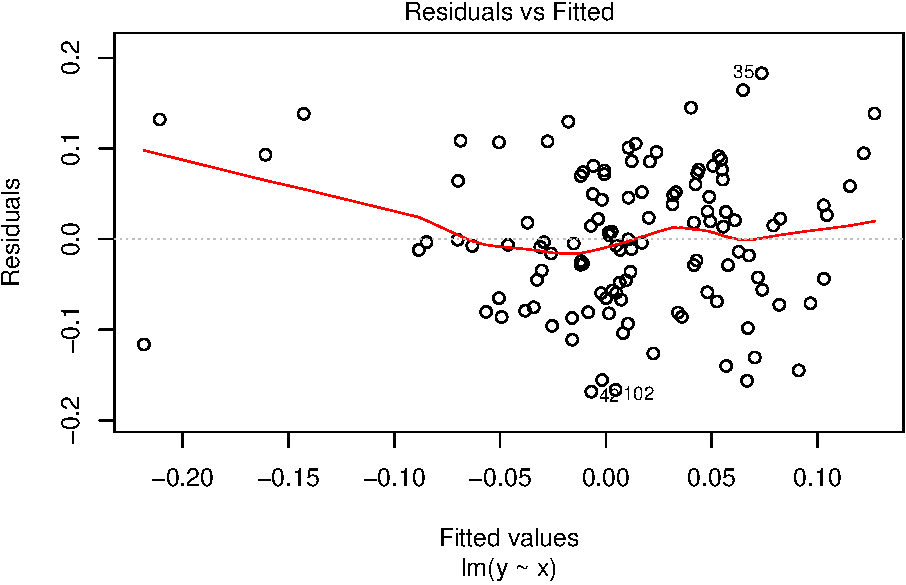
\includegraphics{02-simplereg_files/figure-latex/plot-1.pdf} 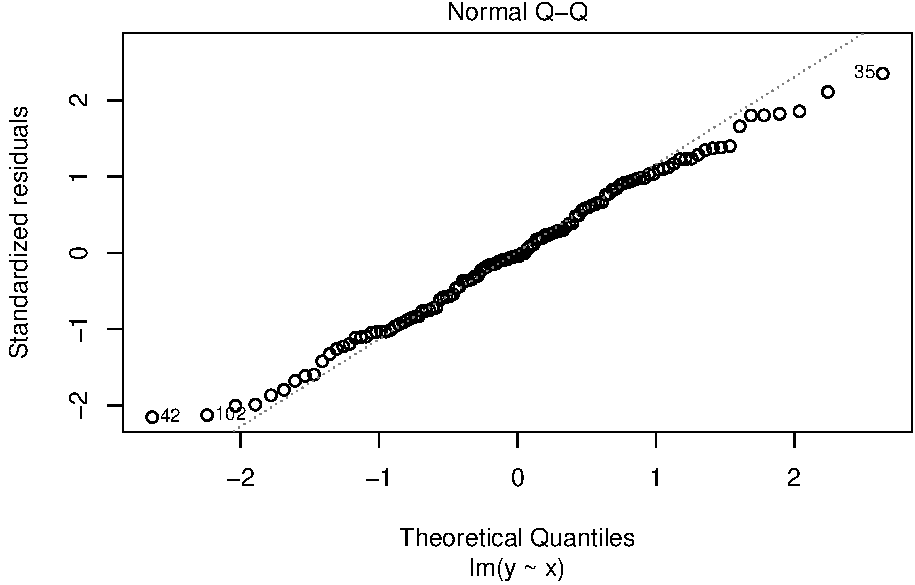
\includegraphics{02-simplereg_files/figure-latex/plot-2.pdf} 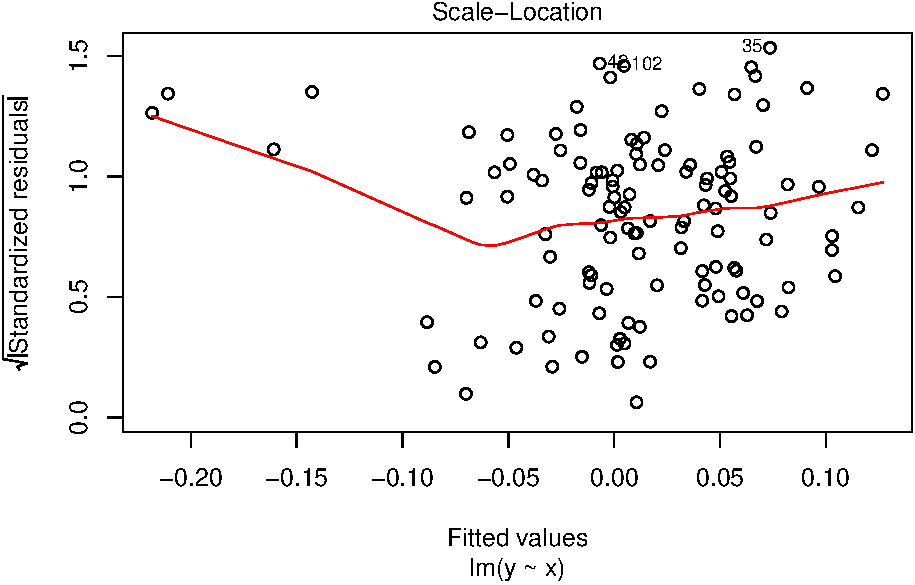
\includegraphics{02-simplereg_files/figure-latex/plot-3.pdf} 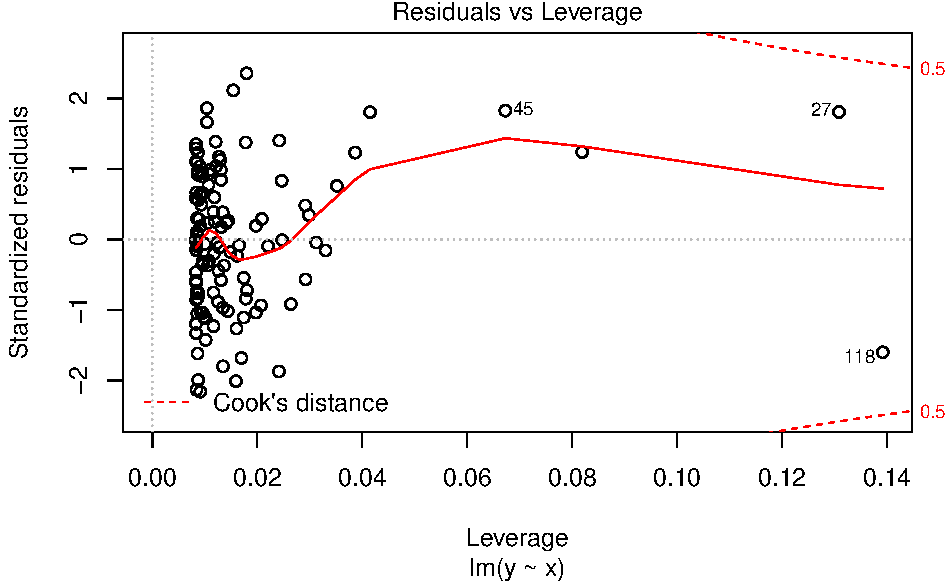
\includegraphics{02-simplereg_files/figure-latex/plot-4.pdf}

Строим доверительный интервал для параметров модели.

\begin{Shaded}
\begin{Highlighting}[]
\NormalTok{est =}\StringTok{ }\KeywordTok{cbind}\NormalTok{(}\DataTypeTok{Estimate =} \KeywordTok{coef}\NormalTok{(ols), }\KeywordTok{confint}\NormalTok{(ols))}
\end{Highlighting}
\end{Shaded}

Проверим гипотезу о равенстве коэффициента при регрессоре единице.

\begin{Shaded}
\begin{Highlighting}[]
\KeywordTok{linearHypothesis}\NormalTok{(ols, }\KeywordTok{c}\NormalTok{(}\StringTok{"x = 1"}\NormalTok{))}
\end{Highlighting}
\end{Shaded}

\begin{verbatim}
Linear hypothesis test

Hypothesis:
x = 1

Model 1: restricted model
Model 2: y ~ x

  Res.Df     RSS Df Sum of Sq      F Pr(>F)
1    119 0.73900                           
2    118 0.72608  1  0.012915 2.0989 0.1501
\end{verbatim}

Посмотрим на остатки :) Протестируем остатки регрессии на нормальность с помощью теста Харке-Бера.

\[
H_{0}: S = 0, K = 3,
\]
где \(S\) --- коэффициент асимметрии (Skewness), \(K\) --- коэффициент эксцесса (Kurtosis)

\begin{Shaded}
\begin{Highlighting}[]
\KeywordTok{jarque.bera.test}\NormalTok{(}\KeywordTok{resid}\NormalTok{(ols)) }
\end{Highlighting}
\end{Shaded}

\begin{verbatim}

    Jarque Bera Test

data:  resid(ols)
X-squared = 1.7803, df = 2, p-value = 0.4106
\end{verbatim}

И тест Шапиро-Уилка.

\(H_{0}: \epsilon_{i} \sim N(\mu,\sigma^2)\)

\begin{Shaded}
\begin{Highlighting}[]
\KeywordTok{shapiro.test}\NormalTok{(}\KeywordTok{resid}\NormalTok{(ols))}
\end{Highlighting}
\end{Shaded}

\begin{verbatim}

    Shapiro-Wilk normality test

data:  resid(ols)
W = 0.99021, p-value = 0.5531
\end{verbatim}

Оба теста указывают на нормальность распределения остатков регрессии.

Сделаем прогноз модели по данным вне обучаемой выборки.

\begin{Shaded}
\begin{Highlighting}[]
\KeywordTok{set.seed}\NormalTok{(}\DecValTok{7}\NormalTok{)}
\NormalTok{newData =}\StringTok{ }\NormalTok{df}
\NormalTok{newData =}\StringTok{ }\KeywordTok{mutate}\NormalTok{(newData, }\DataTypeTok{x =}\NormalTok{ x }\OperatorTok{+}\StringTok{ }\KeywordTok{rnorm}\NormalTok{(}\DataTypeTok{n =} \KeywordTok{n}\NormalTok{())) }\CommentTok{# пошумим}
\NormalTok{yhat =}\StringTok{ }\KeywordTok{predict}\NormalTok{(ols, }\DataTypeTok{newdata =}\NormalTok{ newData, }\DataTypeTok{se =} \OtherTok{TRUE}\NormalTok{)}
\end{Highlighting}
\end{Shaded}

\hypertarget{----}{%
\subsubsection{То же самое в стате}\label{----}}

Загружаем данные.

\begin{verbatim}
use us-return.dta
\end{verbatim}

\begin{verbatim}
end of do-file
\end{verbatim}

Любуемся и даем новые названия столбцам.

\begin{verbatim}
summarize
ren A n
ren B date
\end{verbatim}

\begin{verbatim}
    Variable |        Obs        Mean    Std. Dev.       Min        Max
-------------+---------------------------------------------------------
           A |        120        60.5    34.78505          1        120
           B |          0
       MOBIL |        120    .0161917    .0803075      -.178       .366
      TEXACO |        120    .0119417    .0797036      -.194       .399
         IBM |        120    .0096167     .059024      -.187        .15
-------------+---------------------------------------------------------
         DEC |        120      .01975    .0991438      -.364       .385
      DATGEN |        120    .0074833    .1275399      -.342       .528
       CONED |        120    .0185083    .0502719      -.139       .151
        PSNH |        120   -.0042167    .1094712      -.485       .318
       WEYER |        120    .0096333    .0850664      -.271        .27
-------------+---------------------------------------------------------
       BOISE |        120     .016675    .0974882      -.274       .379
       MOTOR |        120    .0181583    .0972656      -.331        .27
       TANDY |        120    .0250083     .127566      -.246       .454
       PANAM |        120    .0035167    .1318054      -.313       .406
       DELTA |        120    .0116917    .0959317       -.26       .289
-------------+---------------------------------------------------------
      CONTIL |        120      -.0011    .1506992        -.6       .974
      CITCRP |        120    .0118583    .0809719      -.282       .318
      GERBER |        120       .0164    .0877379      -.288       .234
      GENMIL |        120    .0165833    .0650403      -.148        .19
      MARKET |        120    .0139917    .0683532       -.26       .148
-------------+---------------------------------------------------------
      RKFREE |        120    .0068386    .0021869     .00207     .01255
      rkfree |        120    .0068386    .0021869     .00207     .01255
\end{verbatim}

Убираем пропущенные значения и создаем новые переменные.

\begin{verbatim}
drop if n == .
gen y = MOTOR - RKFREE
gen x = MARKET - RKFREE
\end{verbatim}

\begin{verbatim}
(2,544 observations deleted)
\end{verbatim}

Строим модель и проверяем гипотезу об адекватности регрессии. Тут же получаем доверительные интервалы для коэффициентов.

\begin{verbatim}
reg y x
\end{verbatim}

\begin{verbatim}
      Source |       SS           df       MS      Number of obs   =       120
-------------+----------------------------------   F(1, 118)       =     65.48
       Model |  .402913404         1  .402913404   Prob > F        =    0.0000
    Residual |  .726081541       118  .006153233   R-squared       =    0.3569
-------------+----------------------------------   Adj R-squared   =    0.3514
       Total |  1.12899494       119  .009487352   Root MSE        =    .07844

------------------------------------------------------------------------------
           y |      Coef.   Std. Err.      t    P>|t|     [95% Conf. Interval]
-------------+----------------------------------------------------------------
           x |   .8481496   .1048138     8.09   0.000     .6405898    1.055709
       _cons |   .0052529   .0071999     0.73   0.467     -.009005    .0195107
------------------------------------------------------------------------------
\end{verbatim}

Проверим гипотезу о равенстве коэффициента при регрессоре единице.

\begin{verbatim}
test x = 1
\end{verbatim}

\begin{verbatim}
 ( 1)  x = 1

       F(  1,   118) =    2.10
            Prob > F =    0.1501
\end{verbatim}

Сделаем предсказание по выборке и сохраним остатки.

\begin{verbatim}
predict u_hat, resid
predict y_hat
\end{verbatim}

\begin{verbatim}
(option xb assumed; fitted values)
\end{verbatim}

Протестируем остатки регрессии на нормальность с помощью теста Харке-Бера.
На самом деле, это не совсем тест Харке-Бера. Оригинальный вариант ассимптотический и в нем нет поправки на размер выборки. В Stata есть. Подробнее здесь \url{https://www.stata.com/manuals13/rsktest.pdf}

\begin{verbatim}
sktest u_hat
\end{verbatim}

\begin{verbatim}
                    Skewness/Kurtosis tests for Normality
                                                          ------ joint ------
    Variable |        Obs  Pr(Skewness)  Pr(Kurtosis) adj chi2(2)   Prob>chi2
-------------+---------------------------------------------------------------
       u_hat |        120     0.8841        0.1027        2.74         0.2539
\end{verbatim}

И тест Шапиро-Уилка. Тут все аналогично R.

\begin{verbatim}
swilk u_hat
\end{verbatim}

\begin{verbatim}
                   Shapiro-Wilk W test for normal data

    Variable |        Obs       W           V         z       Prob>z
-------------+------------------------------------------------------
       u_hat |        120    0.99021      0.942    -0.133    0.55310
\end{verbatim}

Гипотеза о нормальности остатков не отвергается.

QQ - график

\begin{verbatim}
qnorm u_hat 
\end{verbatim}

\begin{verbatim}

График предсказанных значений против остатков.

```stata
rvfplot, yline(0)
```
\end{verbatim}

График диагональных элементов матрицы-шляпницы против квадрата остатков (по сравнению с R оси поменялись местами).

\begin{verbatim}
lvr2plot
\end{verbatim}

\begin{verbatim}

График предсказанных значений против стандартизиованных остатков. Размер точек на графике зависит от расстояния Кука для данного наблюдения.

```stata
predict D, cooksd
predict standard, rstandard

graph twoway scatter standard y_hat [aweight=D], msymbol(oh) yline(0)
```

```

```



```stata
set seed 7

set obs 120
gen x_new = x+ 0.5 *rnormal()
gen y_hat_new =  .8481496 * x_new+ .0052529
```

```
number of observations (_N) was 120, now 120

```
#### То же самое в python

Много хорошихх функций для статистических расчетов можно найти в пакете Statsmodels. 

```python

import pandas as pd # для работы с таблицами
```

```
Error in py_call_impl(callable, dots$args, dots$keywords): ModuleNotFoundError: No module named 'pandas'

Detailed traceback: 
  File "<string>", line 1, in <module>
```

```python
import numpy as np # математика, работа с матрицами
import matplotlib.pyplot as plt # графики
```

```
Error in py_call_impl(callable, dots$args, dots$keywords): ModuleNotFoundError: No module named 'matplotlib'

Detailed traceback: 
  File "<string>", line 1, in <module>
```

```python
import statsmodels.api as sm
```

```
Error in py_call_impl(callable, dots$args, dots$keywords): ModuleNotFoundError: No module named 'statsmodels'

Detailed traceback: 
  File "<string>", line 1, in <module>
```

```python
import statsmodels.formula.api as smf
```

```
Error in py_call_impl(callable, dots$args, dots$keywords): ModuleNotFoundError: No module named 'statsmodels'

Detailed traceback: 
  File "<string>", line 1, in <module>
```

```python
import statsmodels.graphics.gofplots as gf
```

```
Error in py_call_impl(callable, dots$args, dots$keywords): ModuleNotFoundError: No module named 'statsmodels'

Detailed traceback: 
  File "<string>", line 1, in <module>
```

```python
from statsmodels.stats.outliers_influence import summary_table
```

```
Error in py_call_impl(callable, dots$args, dots$keywords): ModuleNotFoundError: No module named 'statsmodels'

Detailed traceback: 
  File "<string>", line 1, in <module>
```

```python
import seaborn as sns # еще более классные графики
```

```
Error in py_call_impl(callable, dots$args, dots$keywords): ModuleNotFoundError: No module named 'seaborn'

Detailed traceback: 
  File "<string>", line 1, in <module>
```

```python
from scipy.stats import shapiro # еще математика
```

```
Error in py_call_impl(callable, dots$args, dots$keywords): ModuleNotFoundError: No module named 'scipy'

Detailed traceback: 
  File "<string>", line 1, in <module>
```

```python
import statsmodels.discrete.discrete_model
```

```
Error in py_call_impl(callable, dots$args, dots$keywords): ModuleNotFoundError: No module named 'statsmodels'

Detailed traceback: 
  File "<string>", line 1, in <module>
```

При желании, можем кастомизировать графики :)

```python
plt.style.use('seaborn')
```

```
Error in py_call_impl(callable, dots$args, dots$keywords): NameError: name 'plt' is not defined

Detailed traceback: 
  File "<string>", line 1, in <module>
```

```python
plt.rc('font', size=14)
```

```
Error in py_call_impl(callable, dots$args, dots$keywords): NameError: name 'plt' is not defined

Detailed traceback: 
  File "<string>", line 1, in <module>
```

```python
plt.rc('figure', titlesize=15)
```

```
Error in py_call_impl(callable, dots$args, dots$keywords): NameError: name 'plt' is not defined

Detailed traceback: 
  File "<string>", line 1, in <module>
```

```python
plt.rc('axes', labelsize=15)
```

```
Error in py_call_impl(callable, dots$args, dots$keywords): NameError: name 'plt' is not defined

Detailed traceback: 
  File "<string>", line 1, in <module>
```

```python
plt.rc('axes', titlesize=15)
```

```
Error in py_call_impl(callable, dots$args, dots$keywords): NameError: name 'plt' is not defined

Detailed traceback: 
  File "<string>", line 1, in <module>
```

Загрузим данные.

```python
df = pd.read_stata('us-return.dta')
```

```
Error in py_call_impl(callable, dots$args, dots$keywords): NameError: name 'pd' is not defined

Detailed traceback: 
  File "<string>", line 1, in <module>
```

Избавимся от наблюдений с пропущенными значенями. 

```python
df.dropna(inplace=True) ##ИСПРАВИТЬ (выкинуть только пропуски целевой и объяснющей)
```

```
Error in py_call_impl(callable, dots$args, dots$keywords): NameError: name 'df' is not defined

Detailed traceback: 
  File "<string>", line 1, in <module>
```

```python
df.reset_index(drop=True, inplace=True)
```

```
Error in py_call_impl(callable, dots$args, dots$keywords): NameError: name 'df' is not defined

Detailed traceback: 
  File "<string>", line 1, in <module>
```

Переименуем столбцы.

```python
df = df.rename(columns={'A':'n', 'B': 'date'})
```

```
Error in py_call_impl(callable, dots$args, dots$keywords): NameError: name 'df' is not defined

Detailed traceback: 
  File "<string>", line 1, in <module>
```


```python
df['y'] = df['MOTOR'] - df['RKFREE']
```

```
Error in py_call_impl(callable, dots$args, dots$keywords): NameError: name 'df' is not defined

Detailed traceback: 
  File "<string>", line 1, in <module>
```

```python
df['x'] = df['MARKET'] - df['RKFREE'] 
```

```
Error in py_call_impl(callable, dots$args, dots$keywords): NameError: name 'df' is not defined

Detailed traceback: 
  File "<string>", line 1, in <module>
```

Строим модель и читаем саммари :)

```python
regr = smf.ols('y~x', data = df).fit()
```

```
Error in py_call_impl(callable, dots$args, dots$keywords): NameError: name 'smf' is not defined

Detailed traceback: 
  File "<string>", line 1, in <module>
```

```python
regr.summary()
```

```
Error in py_call_impl(callable, dots$args, dots$keywords): NameError: name 'regr' is not defined

Detailed traceback: 
  File "<string>", line 1, in <module>
```

Получить прогноз.

```python
df['yhat'] = regr.fittedvalues
```

```
Error in py_call_impl(callable, dots$args, dots$keywords): NameError: name 'regr' is not defined

Detailed traceback: 
  File "<string>", line 1, in <module>
```

Красивые графики для остатков, выборосов и прочих радостей, как в R, придется строить ручками. Зато приятно поиграть с оформлением :)

```python
fig, ax = plt.subplots()
```

```
Error in py_call_impl(callable, dots$args, dots$keywords): NameError: name 'plt' is not defined

Detailed traceback: 
  File "<string>", line 1, in <module>
```

```python
ax.plot(df['x'],regr.fittedvalues, color='g', alpha =0.8)
```

```
Error in py_call_impl(callable, dots$args, dots$keywords): NameError: name 'ax' is not defined

Detailed traceback: 
  File "<string>", line 1, in <module>
```

```python
ax.scatter(df['x'],regr.fittedvalues+regr.resid, color = 'g', alpha = 0.8, s = 40)
```

```
Error in py_call_impl(callable, dots$args, dots$keywords): NameError: name 'ax' is not defined

Detailed traceback: 
  File "<string>", line 1, in <module>
```

```python
ax.vlines(df['x'],regr.fittedvalues,regr.fittedvalues+regr.resid, color = 'gray', alpha = 0.5)
```

```
Error in py_call_impl(callable, dots$args, dots$keywords): NameError: name 'ax' is not defined

Detailed traceback: 
  File "<string>", line 1, in <module>
```

```python
plt.title('Линия регрессии и остатки')
```

```
Error in py_call_impl(callable, dots$args, dots$keywords): NameError: name 'plt' is not defined

Detailed traceback: 
  File "<string>", line 1, in <module>
```

```python
plt.xlabel('RKFREE')
```

```
Error in py_call_impl(callable, dots$args, dots$keywords): NameError: name 'plt' is not defined

Detailed traceback: 
  File "<string>", line 1, in <module>
```

```python
plt.ylabel('MARKET')
```

```
Error in py_call_impl(callable, dots$args, dots$keywords): NameError: name 'plt' is not defined

Detailed traceback: 
  File "<string>", line 1, in <module>
```

```python
plt.show()
```

```
Error in py_call_impl(callable, dots$args, dots$keywords): NameError: name 'plt' is not defined

Detailed traceback: 
  File "<string>", line 1, in <module>
```

Строим доверительный интервал.

```python
regr.conf_int()
```

```
Error in py_call_impl(callable, dots$args, dots$keywords): NameError: name 'regr' is not defined

Detailed traceback: 
  File "<string>", line 1, in <module>
```

И проведем F-test.

```python
hypotheses = '(x = 1)'
regr.f_test(r_matrix = hypotheses)
```

```
Error in py_call_impl(callable, dots$args, dots$keywords): NameError: name 'regr' is not defined

Detailed traceback: 
  File "<string>", line 1, in <module>
```

Тест Шапиро. Такой же, как и в R. Для удобства можно поместить в табличку.

```python
W, p_value = shapiro(regr.resid)
#pd.DataFrame(data = {'W': [round(W,3)], 'p_value': [round(p_value,3)]})
```

```
Error in py_call_impl(callable, dots$args, dots$keywords): NameError: name 'shapiro' is not defined

Detailed traceback: 
  File "<string>", line 1, in <module>
```


Генерируем новые данные и строим предсказание.

```python
import random
random.seed(7)

newData = df['x'] + 0.5*np.random.normal(len(df))
```

```
Error in py_call_impl(callable, dots$args, dots$keywords): NameError: name 'df' is not defined

Detailed traceback: 
  File "<string>", line 1, in <module>
```

```python
prediction = regr.predict(newData)
```

```
Error in py_call_impl(callable, dots$args, dots$keywords): NameError: name 'regr' is not defined

Detailed traceback: 
  File "<string>", line 1, in <module>
```

А теперь жесть! Построим графички, похожие на autoplot R.


```python
fig_1 = plt.figure(1)
```

```
Error in py_call_impl(callable, dots$args, dots$keywords): NameError: name 'plt' is not defined

Detailed traceback: 
  File "<string>", line 1, in <module>
```

```python
fig_1.axes[0] = sns.residplot(df['x'], df['y'],
                                  lowess=True,
                                  scatter_kws={'alpha': 0.6},
                                  line_kws={'color': 'red', 'lw': 2, 'alpha': 0.8})
```

```
Error in py_call_impl(callable, dots$args, dots$keywords): NameError: name 'sns' is not defined

Detailed traceback: 
  File "<string>", line 1, in <module>
```

```python
fig_1.axes[0].set_title('Residuals vs Fitted')
```

```
Error in py_call_impl(callable, dots$args, dots$keywords): NameError: name 'fig_1' is not defined

Detailed traceback: 
  File "<string>", line 1, in <module>
```

```python
fig_1.axes[0].set_xlabel('Fitted values')
```

```
Error in py_call_impl(callable, dots$args, dots$keywords): NameError: name 'fig_1' is not defined

Detailed traceback: 
  File "<string>", line 1, in <module>
```

```python
fig_1.axes[0].set_ylabel('Residuals')


#можем добавить метки потенциальных аутлаеров
```

```
Error in py_call_impl(callable, dots$args, dots$keywords): NameError: name 'fig_1' is not defined

Detailed traceback: 
  File "<string>", line 1, in <module>
```

```python
abs_resid = abs(regr.resid).sort_values(ascending=False)
```

```
Error in py_call_impl(callable, dots$args, dots$keywords): NameError: name 'regr' is not defined

Detailed traceback: 
  File "<string>", line 1, in <module>
```

```python
abs_resid_top3 = abs_resid[:3]
```

```
Error in py_call_impl(callable, dots$args, dots$keywords): NameError: name 'abs_resid' is not defined

Detailed traceback: 
  File "<string>", line 1, in <module>
```

```python
for i in abs_resid_top3.index:
    fig_1.axes[0].annotate(i, 
                               xy=(regr.fittedvalues[i], 
                                   regr.resid[i]))
```

```
Error in py_call_impl(callable, dots$args, dots$keywords): NameError: name 'abs_resid_top3' is not defined

Detailed traceback: 
  File "<string>", line 1, in <module>
```



```python
norm_residuals = regr.get_influence().resid_studentized_internal #сохраним стьюдентизированные остатки 

```

```
Error in py_call_impl(callable, dots$args, dots$keywords): NameError: name 'regr' is not defined

Detailed traceback: 
  File "<string>", line 1, in <module>
```

```python
QQ = gf.ProbPlot(norm_residuals)
```

```
Error in py_call_impl(callable, dots$args, dots$keywords): NameError: name 'gf' is not defined

Detailed traceback: 
  File "<string>", line 1, in <module>
```

```python
fig_2 = QQ.qqplot(line='45', alpha=0.5, color='b', lw=1)

```

```
Error in py_call_impl(callable, dots$args, dots$keywords): NameError: name 'QQ' is not defined

Detailed traceback: 
  File "<string>", line 1, in <module>
```

```python
fig_2.axes[0].set_title('Normal Q-Q')
```

```
Error in py_call_impl(callable, dots$args, dots$keywords): NameError: name 'fig_2' is not defined

Detailed traceback: 
  File "<string>", line 1, in <module>
```

```python
fig_2.axes[0].set_xlabel('Theoretical Quantiles')
```

```
Error in py_call_impl(callable, dots$args, dots$keywords): NameError: name 'fig_2' is not defined

Detailed traceback: 
  File "<string>", line 1, in <module>
```

```python
fig_2.axes[0].set_ylabel('Standardized Residuals');

#и снова метки
```

```
Error in py_call_impl(callable, dots$args, dots$keywords): NameError: name 'fig_2' is not defined

Detailed traceback: 
  File "<string>", line 1, in <module>
```

```python
abs_norm_resid = np.flip(np.argsort(abs(norm_residuals)), 0)
```

```
Error in py_call_impl(callable, dots$args, dots$keywords): NameError: name 'norm_residuals' is not defined

Detailed traceback: 
  File "<string>", line 1, in <module>
```

```python
abs_norm_resid_top3 = abs_norm_resid[:3]
```

```
Error in py_call_impl(callable, dots$args, dots$keywords): NameError: name 'abs_norm_resid' is not defined

Detailed traceback: 
  File "<string>", line 1, in <module>
```

```python
for r, i in enumerate(abs_norm_resid_top3):
    fig_2.axes[0].annotate(i, 
                               xy=(np.flip(QQ.theoretical_quantiles, 0)[r],
                                   norm_residuals[i]))
```

```
Error in py_call_impl(callable, dots$args, dots$keywords): NameError: name 'abs_norm_resid_top3' is not defined

Detailed traceback: 
  File "<string>", line 1, in <module>
```



```python
fig_3 = plt.figure(3)
```

```
Error in py_call_impl(callable, dots$args, dots$keywords): NameError: name 'plt' is not defined

Detailed traceback: 
  File "<string>", line 1, in <module>
```

```python
plt.scatter(regr.fittedvalues, np.sqrt(abs(norm_residuals)), alpha=0.5)
```

```
Error in py_call_impl(callable, dots$args, dots$keywords): NameError: name 'plt' is not defined

Detailed traceback: 
  File "<string>", line 1, in <module>
```

```python
sns.regplot(regr.fittedvalues, np.sqrt(abs(norm_residuals)), 
            scatter=False, 
            ci=False, 
            lowess=True,
            line_kws={'color': 'red', 'lw': 1, 'alpha': 0.6})
```

```
Error in py_call_impl(callable, dots$args, dots$keywords): NameError: name 'sns' is not defined

Detailed traceback: 
  File "<string>", line 1, in <module>
```

```python
fig_3.axes[0].set_title('Scale-Location')
```

```
Error in py_call_impl(callable, dots$args, dots$keywords): NameError: name 'fig_3' is not defined

Detailed traceback: 
  File "<string>", line 1, in <module>
```

```python
fig_3.axes[0].set_xlabel('Fitted values')
```

```
Error in py_call_impl(callable, dots$args, dots$keywords): NameError: name 'fig_3' is not defined

Detailed traceback: 
  File "<string>", line 1, in <module>
```

```python
fig_3.axes[0].set_ylabel('$\sqrt{|Standardized Residuals|}$')

# и еще раз!)
```

```
Error in py_call_impl(callable, dots$args, dots$keywords): NameError: name 'fig_3' is not defined

Detailed traceback: 
  File "<string>", line 1, in <module>
```

```python
abs_sq_norm_resid = np.flip(np.argsort(np.sqrt(abs(norm_residuals)), 0))
```

```
Error in py_call_impl(callable, dots$args, dots$keywords): NameError: name 'norm_residuals' is not defined

Detailed traceback: 
  File "<string>", line 1, in <module>
```

```python
abs_sq_norm_resid_top3 = abs_sq_norm_resid[:3]
```

```
Error in py_call_impl(callable, dots$args, dots$keywords): NameError: name 'abs_sq_norm_resid' is not defined

Detailed traceback: 
  File "<string>", line 1, in <module>
```

```python
for i in abs_sq_norm_resid_top3:
    fig_3.axes[0].annotate(i, xy=(regr.fittedvalues[i], 
                                   np.sqrt(abs(norm_residuals)[i])))
```

```
Error in py_call_impl(callable, dots$args, dots$keywords): NameError: name 'abs_sq_norm_resid_top3' is not defined

Detailed traceback: 
  File "<string>", line 1, in <module>
```


```python
leverage = regr.get_influence().hat_matrix_diag #сохраняем элементы матрицы-шляпницы
```

```
Error in py_call_impl(callable, dots$args, dots$keywords): NameError: name 'regr' is not defined

Detailed traceback: 
  File "<string>", line 1, in <module>
```

```python
cook_dist = regr.get_influence().cooks_distance[0] #И расстояние Кука
```

```
Error in py_call_impl(callable, dots$args, dots$keywords): NameError: name 'regr' is not defined

Detailed traceback: 
  File "<string>", line 1, in <module>
```

```python
fig_4 = plt.figure(4)
```

```
Error in py_call_impl(callable, dots$args, dots$keywords): NameError: name 'plt' is not defined

Detailed traceback: 
  File "<string>", line 1, in <module>
```

```python
plt.scatter(leverage, norm_residuals, alpha=0.5)
```

```
Error in py_call_impl(callable, dots$args, dots$keywords): NameError: name 'plt' is not defined

Detailed traceback: 
  File "<string>", line 1, in <module>
```

```python
sns.regplot(leverage, norm_residuals, 
            scatter=False, 
            ci=False, 
            lowess=True,
            line_kws={'color': 'red', 'lw': 1, 'alpha': 0.8})
```

```
Error in py_call_impl(callable, dots$args, dots$keywords): NameError: name 'sns' is not defined

Detailed traceback: 
  File "<string>", line 1, in <module>
```

```python
fig_4.axes[0].set_xlim(0, 0.20)
```

```
Error in py_call_impl(callable, dots$args, dots$keywords): NameError: name 'fig_4' is not defined

Detailed traceback: 
  File "<string>", line 1, in <module>
```

```python
fig_4.axes[0].set_ylim(-3, 5)
```

```
Error in py_call_impl(callable, dots$args, dots$keywords): NameError: name 'fig_4' is not defined

Detailed traceback: 
  File "<string>", line 1, in <module>
```

```python
fig_4.axes[0].set_title('Residuals vs Leverage')
```

```
Error in py_call_impl(callable, dots$args, dots$keywords): NameError: name 'fig_4' is not defined

Detailed traceback: 
  File "<string>", line 1, in <module>
```

```python
fig_4.axes[0].set_xlabel('Leverage')
```

```
Error in py_call_impl(callable, dots$args, dots$keywords): NameError: name 'fig_4' is not defined

Detailed traceback: 
  File "<string>", line 1, in <module>
```

```python
fig_4.axes[0].set_ylabel('Standardized Residuals')

```

```
Error in py_call_impl(callable, dots$args, dots$keywords): NameError: name 'fig_4' is not defined

Detailed traceback: 
  File "<string>", line 1, in <module>
```

```python
leverage_top3 = np.flip(np.argsort(cook_dist), 0)[:3]
```

```
Error in py_call_impl(callable, dots$args, dots$keywords): NameError: name 'cook_dist' is not defined

Detailed traceback: 
  File "<string>", line 1, in <module>
```

```python
for i in leverage_top3:
    fig_4.axes[0].annotate(i, 
                               xy=(leverage[i], 
                                   norm_residuals[i]))
```

```
Error in py_call_impl(callable, dots$args, dots$keywords): NameError: name 'leverage_top3' is not defined

Detailed traceback: 
  File "<string>", line 1, in <module>
```

```python
plt.show()
```

```
Error in py_call_impl(callable, dots$args, dots$keywords): NameError: name 'plt' is not defined

Detailed traceback: 
  File "<string>", line 1, in <module>
```


<!--chapter:end:02-simplereg.Rmd-->

# Модели бинарного выбора {#binchoice}


<!--chapter:end:03-binchoice.Rmd-->

# Модели упорядоченного выбора и условный логит {#ordchoice}




Загрузим необходимые пакеты.

```r
library(tidyverse) # для манипуляций с данными и построения графиков
library(skimr) #для красивого summary
library(rio) # для чтения .dta файлов
library(margins)
```

```
Error in library(margins): there is no package called 'margins'
```

```r
library(mlogit)
```

```
Error in library(mlogit): there is no package called 'mlogit'
```

```r
library(nnet)
library(questionr)
```

```
Error in library(questionr): there is no package called 'questionr'
```

```r
library(MASS)
library(survival)

# log(6)
```

Импортируем датасет. В нем находятся данные по клиентам пенсионных фондов. Нас интересует переменная `pctstck`, которая принимает три значения: 0, 50, 100 - в зависимоcти от ответа респондента на вопрос о предпочтительном способе инвестирования пенсионных накоплений.   

```r
df = rio::import("pension.dta")
```


```r
skim_with(numeric = list(hist = NULL, p25 = NULL, p75 = NULL)) #посмотрим на данные
#skim(df)
```


Создадим факторную перменную и упорядочим категории. 


```r
df = rename(df,  alloc = pctstck) # переименуем 
df = mutate(df, alloc_factor = factor(alloc)) # факторная переменная
df = mutate(df, y = relevel(df$alloc_factor, ref = 1)) # сменить базовую категорию
levels(df$y)
```

```
[1] "0"   "50"  "100"
```

Построим модель множественного выбора (лог-линейная модель). 

```r
multmodel = multinom(y ~ choice+age+educ+wealth89+prftshr, data = df)
```

```
# weights:  21 (12 variable)
initial  value 220.821070 
iter  10 value 207.012642
iter  20 value 204.507792
final  value 204.507779 
converged
```

```r
summary(multmodel)
```

```
Call:
multinom(formula = y ~ choice + age + educ + wealth89 + prftshr, 
    data = df)

Coefficients:
    (Intercept)    choice         age       educ      wealth89    prftshr
50     3.777686 0.6269410 -0.10621691 0.18518113 -0.0003716626 -0.2717872
100    4.492971 0.6244954 -0.09482129 0.04644315 -0.0003548369  0.9809245

Std. Errors:
    (Intercept)    choice        age       educ     wealth89   prftshr
50     1.581691 0.3701263 0.02826469 0.06725443 0.0007365833 0.4988234
100    1.385291 0.3851273 0.02530600 0.07203058 0.0007896235 0.4396202

Residual Deviance: 409.0156 
AIC: 433.0156 
```

Сохраним прогнозы.

```r
fit_values = fitted(multmodel)
head(fit_values)
```

```
          0        50       100
1 0.4040703 0.3308134 0.2651163
2 0.1534943 0.2619464 0.5845593
3 0.1651913 0.2342525 0.6005562
4 0.4300671 0.1504960 0.4194370
5 0.4878942 0.2797337 0.2323721
6 0.4642700 0.1265789 0.4091510
```

И посчитать относительное изменение отношения шансов:

\[
\frac{P(y_{i} = j)}{P(y_{i} = 1)} = exp(x_{i}\beta)
\] 
показывает изменение отношения шансов при выборе альтернативы j вместо альтернативы 0, если x изменился на единицу

```r
odds.ratio(multmodel) # отношение шансов в stata называется relative-risk ratio
```

```
Error in odds.ratio(multmodel): could not find function "odds.ratio"
```


Можем посчитать предельные эффекты в различных квартилях. 

```r
summary(marginal_effects(multmodel)) # mean как в стате
```

```
Error in marginal_effects(multmodel): could not find function "marginal_effects"
```



Допустим, мы можем упорядочить наши альтернативы (например, от более рискованного способа распределения ресурсов до менее)

```r
ordered_logit = polr(y ~ choice+age+educ+wealth89+prftshr , data = df)
ordered_probit = polr(y ~ choice+age+educ+wealth89+prftshr , data = df, method = 'probit') 

fit_prob = fitted(ordered_probit)
fit_log = fitted(ordered_logit)
ordered_probit
```

```
Call:
polr(formula = y ~ choice + age + educ + wealth89 + prftshr, 
    data = df, method = "probit")

Coefficients:
       choice           age          educ      wealth89       prftshr 
 0.2932276690 -0.0453064786  0.0269376562 -0.0001693805  0.4864824791 

Intercepts:
     0|50    50|100 
-2.578050 -1.561799 

Residual Deviance: 425.7763 
AIC: 439.7763 
(25 observations deleted due to missingness)
```

```r
ln(5)
```

```
Error in ln(5): could not find function "ln"
```



```r
cond_logit = clogit(y ~ choice+age+strata(educ)+wealth89+prftshr , data = df)
```

```
Error in coxph(formula = Surv(rep(1, 226L), y) ~ choice + age + strata(educ) + : Cox model doesn't support "mright" survival data
```

### То же самое в стате



```stata
use pension.dta
```

```
end of do-file
```


```stata
sum
```

```
    Variable |        Obs        Mean    Std. Dev.       Min        Max
-------------+---------------------------------------------------------
          id |        226    2445.093    1371.271         38       5014
      pyears |        218    11.38532    9.605498          0         45
     prftshr |        206    .2087379    .4073967          0          1
      choice |        226    .6150442     .487665          0          1
      female |        226    .6017699      .49062          0          1
-------------+---------------------------------------------------------
     married |        226    .7345133    .4425723          0          1
         age |        226    60.70354    4.287002         53         73
        educ |        219    13.51598    2.554627          8         18
      finc25 |        216    .2083333    .4070598          0          1
      finc35 |        216    .1851852      .38935          0          1
-------------+---------------------------------------------------------
      finc50 |        216    .2453704    .4313061          0          1
      finc75 |        216        .125    .3314871          0          1
     finc100 |        216    .1203704      .32615          0          1
     finc101 |        216    .0648148    .2467707          0          1
    wealth89 |        226    197.9057    242.0919   -579.997   1484.997
-------------+---------------------------------------------------------
       black |        226     .119469    .3250596          0          1
    stckin89 |        226    .3185841    .4669616          0          1
     irain89 |        226          .5    .5011099          0          1
     pctstck |        226    46.68142    39.44116          0        100
```



```stata
ren pctstck alloc
```
\end{verbatim}

Построим модель множественного выбора (лог-линейная модель).

\begin{verbatim}
mlogit alloc choice age educ wealth89 prftshr,  baseoutcome(0) #маленькое отличие с R
\end{verbatim}

\begin{verbatim}
> ичие с R
option # not allowed
r(198);

end of do-file
r(198);
\end{verbatim}

Можем посмотреть на прогнозы.

\begin{verbatim}
predict p1 p2 p3, p
\end{verbatim}

\begin{verbatim}
 option # not allowed
r(198);


last estimates not found
r(301);

end of do-file
r(301);
\end{verbatim}

И посчитать относительное изменение отношения шансов:

\[
\frac{P(y_{i} = j)}{P(y_{i} = 1)} = exp(x_{i}\beta)
\] - показывает изменение отношения шансов при выборе альтернативы j вместо альтернативы 0, если x изменился на единицу

\begin{verbatim}
mlogit, rrr #relative-risk ratio
\end{verbatim}

\begin{verbatim}
 option # not allowed
r(198);


last estimates not found
r(301);

end of do-file
r(301);
\end{verbatim}

Можем посчитать предельные эффекты в разных точках.

\begin{verbatim}
margins, predict(outcome(50)) dydx( choice age educ wealth89 prftshr) atmeans 

margins, predict(outcome(50)) dydx( choice age educ wealth89 prftshr) at((p25) *)
\end{verbatim}

\begin{verbatim}
 option # not allowed
r(198);


last estimates not found
r(301);

end of do-file
r(301);
\end{verbatim}

\begin{verbatim}
oprobit alloc choice age educ wealth89 prftshr

ologit alloc choice age educ wealth89 prftshr
\end{verbatim}

\begin{verbatim}
 option # not allowed
r(198);



Iteration 0:   log likelihood = -219.86356  
Iteration 1:   log likelihood = -212.89234  
Iteration 2:   log likelihood = -212.88817  
Iteration 3:   log likelihood = -212.88817  

Ordered probit regression                       Number of obs     =        201
                                                LR chi2(5)        =      13.95
                                                Prob > chi2       =     0.0159
Log likelihood = -212.88817                     Pseudo R2         =     0.0317

------------------------------------------------------------------------------
       alloc |      Coef.   Std. Err.      z    P>|z|     [95% Conf. Interval]
-------------+----------------------------------------------------------------
      choice |   .2932272    .167064     1.76   0.079    -.0342122    .6206666
         age |  -.0453065   .0195009    -2.32   0.020    -.0835275   -.0070854
        educ |   .0269375   .0315643     0.85   0.393    -.0349273    .0888024
    wealth89 |  -.0001694   .0003431    -0.49   0.622    -.0008419    .0005031
     prftshr |   .4864833   .2030406     2.40   0.017      .088531    .8844355
-------------+----------------------------------------------------------------
       /cut1 |  -2.578052   1.277878                     -5.082648   -.0734562
       /cut2 |  -1.561798   1.272756                     -4.056353    .9327576
------------------------------------------------------------------------------


Iteration 0:   log likelihood = -219.86356  
Iteration 1:   log likelihood = -212.75117  
Iteration 2:   log likelihood = -212.72813  
Iteration 3:   log likelihood = -212.72813  

Ordered logistic regression                     Number of obs     =        201
                                                LR chi2(5)        =      14.27
                                                Prob > chi2       =     0.0140
Log likelihood = -212.72813                     Pseudo R2         =     0.0325

------------------------------------------------------------------------------
       alloc |      Coef.   Std. Err.      z    P>|z|     [95% Conf. Interval]
-------------+----------------------------------------------------------------
      choice |   .4720438   .2757545     1.71   0.087     -.068425    1.012513
         age |  -.0776337   .0328659    -2.36   0.018    -.1420497   -.0132177
        educ |   .0475714   .0514763     0.92   0.355    -.0533203    .1484631
    wealth89 |   -.000277    .000561    -0.49   0.621    -.0013765    .0008224
     prftshr |   .8312158   .3506528     2.37   0.018     .1439489    1.518483
-------------+----------------------------------------------------------------
       /cut1 |  -4.376271   2.144494                     -8.579402   -.1731395
       /cut2 |  -2.714186   2.129423                     -6.887779    1.459407
------------------------------------------------------------------------------
\end{verbatim}

Посмотрим на conditional logit

ПОКА ЗАБИЛА

\begin{verbatim}

use crackers.dta


egen resp = group(id occ)

tabulate brand, generate(br)
rename br1 Sunshine
rename br2 Keebler
rename br3 Nabisco

clogit choice Sunshine Keebler Nabisco display feature price, group(resp)
\end{verbatim}

\begin{verbatim}
 option # not allowed
r(198);


no; data in memory would be lost
r(4);

end of do-file
r(4);
\end{verbatim}

\hypertarget{poisreg}{%
\chapter{Модели счетных данных}\label{poisreg}}

Загрузим необходимые пакеты.

\begin{Shaded}
\begin{Highlighting}[]
\KeywordTok{library}\NormalTok{(tidyverse) }\CommentTok{#работа с данными и графики}
\KeywordTok{library}\NormalTok{(skimr) }\CommentTok{#красивое summary}
\KeywordTok{library}\NormalTok{(rio) }\CommentTok{#чтение .dta файлов}
\KeywordTok{library}\NormalTok{(vcd) }\CommentTok{#еще графики}
\KeywordTok{library}\NormalTok{(MASS) }\CommentTok{#отрицательное биномиальное}
\KeywordTok{library}\NormalTok{(lmtest) }\CommentTok{#для проверки гипотез}
\KeywordTok{library}\NormalTok{(pscl) }\CommentTok{#zero-inflation function}
\end{Highlighting}
\end{Shaded}

\begin{verbatim}
Error in library(pscl): there is no package called 'pscl'
\end{verbatim}

\begin{Shaded}
\begin{Highlighting}[]
\KeywordTok{library}\NormalTok{(margins) }\CommentTok{#для подсчета предельных эффектов}
\end{Highlighting}
\end{Shaded}

\begin{verbatim}
Error in library(margins): there is no package called 'margins'
\end{verbatim}

Импортируем данные.

\begin{Shaded}
\begin{Highlighting}[]
\NormalTok{df =}\StringTok{ }\KeywordTok{import}\NormalTok{(}\DataTypeTok{file =} \StringTok{"fish.dta"}\NormalTok{)}
\end{Highlighting}
\end{Shaded}

Данные содержат информацию о количестве рыбы, пойманной людьми на отдыхе.

Camper - наличие/отсутсвие палатки.
Child - количество детей, которых взяли на рыбалку.
Persons - количество людей в группе.
Count - количество пойманной рыбы

Посмотрим нам описательные статистики.

\begin{Shaded}
\begin{Highlighting}[]
\KeywordTok{skim_with}\NormalTok{(}\DataTypeTok{numeric =} \KeywordTok{list}\NormalTok{(}\DataTypeTok{hist =} \OtherTok{NULL}\NormalTok{, }\DataTypeTok{p25 =} \OtherTok{NULL}\NormalTok{, }\DataTypeTok{p75 =} \OtherTok{NULL}\NormalTok{))}
\KeywordTok{skim}\NormalTok{(df)}
\end{Highlighting}
\end{Shaded}

\begin{verbatim}
Skim summary statistics
 n obs: 250 
 n variables: 4 

-- Variable type:numeric ------------------------
 variable missing complete   n mean    sd p0 p50 p100
   camper       0      250 250 0.59  0.49  0   1    1
    child       0      250 250 0.68  0.85  0   0    3
    count       0      250 250 3.3  11.64  0   0  149
  persons       0      250 250 2.53  1.11  1   2    4
\end{verbatim}

Переменная \texttt{camper} принимает всего два значения, поэтому превратим ее в факторную переменную.

\begin{Shaded}
\begin{Highlighting}[]
\NormalTok{df =}\StringTok{ }\KeywordTok{mutate}\NormalTok{(df, }\DataTypeTok{camper =} \KeywordTok{factor}\NormalTok{(camper))}
\end{Highlighting}
\end{Shaded}

Наша задача - по имеющимся данным предсказать улов. Для начала посмотрим на распределение объясняемой переменной \texttt{count}.

\begin{Shaded}
\begin{Highlighting}[]
\KeywordTok{ggplot}\NormalTok{(df, }\KeywordTok{aes}\NormalTok{(}\DataTypeTok{x =}\NormalTok{ count)) }\OperatorTok{+}\StringTok{ }\KeywordTok{geom_histogram}\NormalTok{(}\DataTypeTok{binwidth =} \DecValTok{1}\NormalTok{) }\OperatorTok{+}\StringTok{ }\KeywordTok{labs}\NormalTok{(}\DataTypeTok{x =} \StringTok{'count'}\NormalTok{, }\DataTypeTok{y =} \StringTok{'frequency'}\NormalTok{, }\DataTypeTok{title =} \StringTok{'Distribution of count variable'}\NormalTok{)}
\end{Highlighting}
\end{Shaded}

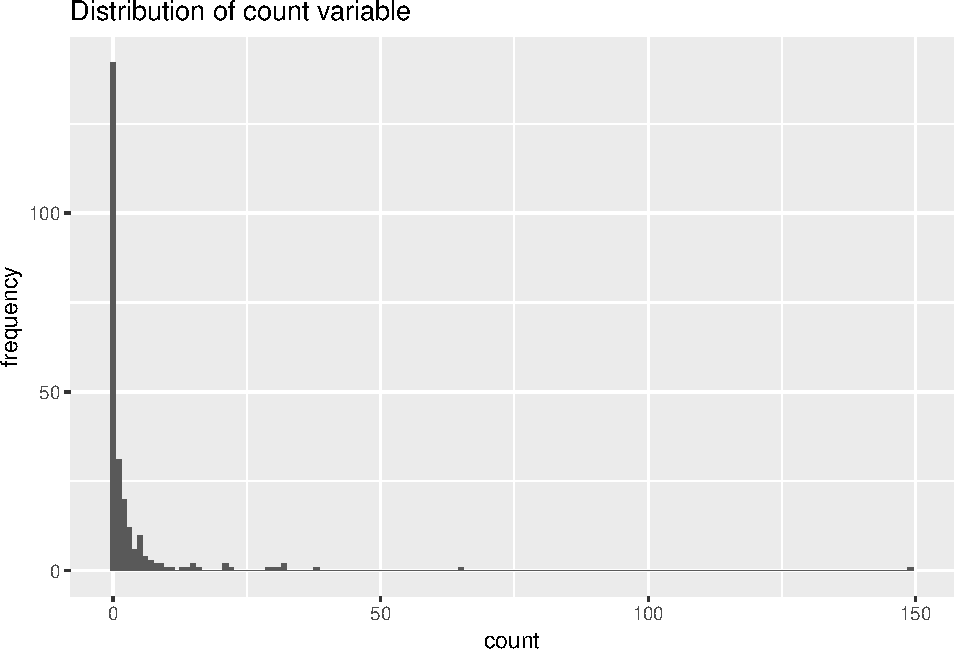
\includegraphics{05-poisreg_files/figure-latex/hist-1.pdf}

Предположим, что переменная имеет распределение Пуассона. Будем использовать пуассоновскую регрессию.
\[
P(y=k)=exp(-\lambda) \lambda^k / k!
\]
где \(\lambda=\exp(b_1 +b_2*x)\)

\begin{Shaded}
\begin{Highlighting}[]
\NormalTok{poisson =}\StringTok{ }\KeywordTok{glm}\NormalTok{(count }\OperatorTok{~}\StringTok{ }\NormalTok{child }\OperatorTok{+}\StringTok{ }\NormalTok{camper }\OperatorTok{+}\StringTok{  }\NormalTok{persons, }\DataTypeTok{family =} \StringTok{"poisson"}\NormalTok{, }\DataTypeTok{data =}\NormalTok{ df)}
\KeywordTok{summary}\NormalTok{(poisson)}
\end{Highlighting}
\end{Shaded}

\begin{verbatim}

Call:
glm(formula = count ~ child + camper + persons, family = "poisson", 
    data = df)

Deviance Residuals: 
    Min       1Q   Median       3Q      Max  
-6.8096  -1.4431  -0.9060  -0.0406  16.1417  

Coefficients:
            Estimate Std. Error z value Pr(>|z|)    
(Intercept) -1.98183    0.15226  -13.02   <2e-16 ***
child       -1.68996    0.08099  -20.87   <2e-16 ***
camper1      0.93094    0.08909   10.45   <2e-16 ***
persons      1.09126    0.03926   27.80   <2e-16 ***
---
Signif. codes:  0 '***' 0.001 '**' 0.01 '*' 0.05 '.' 0.1 ' ' 1

(Dispersion parameter for poisson family taken to be 1)

    Null deviance: 2958.4  on 249  degrees of freedom
Residual deviance: 1337.1  on 246  degrees of freedom
AIC: 1682.1

Number of Fisher Scoring iterations: 6
\end{verbatim}

Посчитаем средний предельный эффект для каждой переменной.

\begin{Shaded}
\begin{Highlighting}[]
\KeywordTok{colMeans}\NormalTok{(}\KeywordTok{marginal_effects}\NormalTok{(poisson))}
\end{Highlighting}
\end{Shaded}

\begin{verbatim}
Error in marginal_effects(poisson): could not find function "marginal_effects"
\end{verbatim}

Однако, заметим, что дисперсия и среднее значение объясняемой переменной не равны, как это предполагает распределение Пуассона.

\begin{Shaded}
\begin{Highlighting}[]
\NormalTok{df }\OperatorTok\StringTok{ }\KeywordTok{group_by}\NormalTok{(camper) }\OperatorTok\StringTok{ }\KeywordTok{summarize}\NormalTok{(}\DataTypeTok{var =} \KeywordTok{var}\NormalTok{(count), }\DataTypeTok{mean =} \KeywordTok{mean}\NormalTok{(count))}
\end{Highlighting}
\end{Shaded}

\begin{verbatim}
# A tibble: 2 x 3
  camper   var  mean
  <fct>  <dbl> <dbl>
1 0       21.1  1.52
2 1      212.   4.54
\end{verbatim}

Оценим регрессию, предполагая отрицательное биномиальное распределение остатков. В этом случае, дисперсия распределения зависит от некоторого параметра и не равна среднему.

\begin{Shaded}
\begin{Highlighting}[]
\NormalTok{nb1 =}\StringTok{ }\KeywordTok{glm.nb}\NormalTok{(count }\OperatorTok{~}\StringTok{ }\NormalTok{child }\OperatorTok{+}\StringTok{ }\NormalTok{camper }\OperatorTok{+}\StringTok{  }\NormalTok{persons, }\DataTypeTok{data =}\NormalTok{ df)}
\KeywordTok{summary}\NormalTok{(nb1)}
\end{Highlighting}
\end{Shaded}

\begin{verbatim}

Call:
glm.nb(formula = count ~ child + camper + persons, data = df, 
    init.theta = 0.4635287626, link = log)

Deviance Residuals: 
    Min       1Q   Median       3Q      Max  
-1.6673  -0.9599  -0.6590  -0.0319   4.9433  

Coefficients:
            Estimate Std. Error z value Pr(>|z|)    
(Intercept)  -1.6250     0.3304  -4.918 8.74e-07 ***
child        -1.7805     0.1850  -9.623  < 2e-16 ***
camper1       0.6211     0.2348   2.645  0.00816 ** 
persons       1.0608     0.1144   9.273  < 2e-16 ***
---
Signif. codes:  0 '***' 0.001 '**' 0.01 '*' 0.05 '.' 0.1 ' ' 1

(Dispersion parameter for Negative Binomial(0.4635) family taken to be 1)

    Null deviance: 394.25  on 249  degrees of freedom
Residual deviance: 210.65  on 246  degrees of freedom
AIC: 820.44

Number of Fisher Scoring iterations: 1

              Theta:  0.4635 
          Std. Err.:  0.0712 

 2 x log-likelihood:  -810.4440 
\end{verbatim}

Попробуем исключить из модели переменную \texttt{camper} и сравним качество двух моделей.

\begin{Shaded}
\begin{Highlighting}[]
\NormalTok{nb2 =}\StringTok{ }\KeywordTok{update}\NormalTok{(nb1, . }\OperatorTok{~}\StringTok{ }\NormalTok{. }\OperatorTok{-}\StringTok{ }\NormalTok{camper)}
\KeywordTok{waldtest}\NormalTok{(nb1, nb2)}
\end{Highlighting}
\end{Shaded}

\begin{verbatim}
Wald test

Model 1: count ~ child + camper + persons
Model 2: count ~ child + persons
  Res.Df Df      F   Pr(>F)   
1    246                      
2    247 -1 6.9979 0.008686 **
---
Signif. codes:  0 '***' 0.001 '**' 0.01 '*' 0.05 '.' 0.1 ' ' 1
\end{verbatim}

Можем посмотреть на результаты модели с ``раздутыми нулями'' (zero-inflated). Они предполагают большую частоту нулевых наблюдений.

\begin{Shaded}
\begin{Highlighting}[]
\NormalTok{zero_infl =}\StringTok{ }\KeywordTok{zeroinfl}\NormalTok{(count }\OperatorTok{~}\StringTok{ }\NormalTok{child }\OperatorTok{+}\StringTok{ }\NormalTok{camper }\OperatorTok{|}\StringTok{ }\NormalTok{persons, }\DataTypeTok{data =}\NormalTok{ df, }\DataTypeTok{dist =} \StringTok{'negbin'}\NormalTok{)}
\end{Highlighting}
\end{Shaded}

\begin{verbatim}
Error in zeroinfl(count ~ child + camper | persons, data = df, dist = "negbin"): could not find function "zeroinfl"
\end{verbatim}

\begin{Shaded}
\begin{Highlighting}[]
\KeywordTok{summary}\NormalTok{(zero_infl)}
\end{Highlighting}
\end{Shaded}

\begin{verbatim}
Error in summary(zero_infl): object 'zero_infl' not found
\end{verbatim}

\hypertarget{-----1}{%
\subsubsection{То же самое в стате}\label{-----1}}

Загружаем данные и смотрим описательные статистики.

\begin{verbatim}
use fish.dta
summarize
\end{verbatim}

\begin{verbatim}
    Variable |        Obs        Mean    Std. Dev.       Min        Max
-------------+---------------------------------------------------------
      camper |        250        .588    .4931824          0          1
       child |        250        .684    .8503153          0          3
       count |        250       3.296    11.63503          0        149
     persons |        250       2.528     1.11273          1          4
\end{verbatim}

\begin{verbatim}
hist count
\end{verbatim}

\begin{verbatim}
(bin=15, start=0, width=9.9333333)
\end{verbatim}

Строим Пуассоновскую регрессию.
В описательных статистиках:
\(AIC = -2log(L) + 2k\)
\(AIC = -2log(L) + klog(N)\)

\begin{verbatim}
glm count camper child persons, family(poisson)
\end{verbatim}

\begin{verbatim}
Iteration 0:   log likelihood = -965.92815  
Iteration 1:   log likelihood = -837.97093  
Iteration 2:   log likelihood = -837.07307  
Iteration 3:   log likelihood = -837.07248  
Iteration 4:   log likelihood = -837.07248  

Generalized linear models                         No. of obs      =        250
Optimization     : ML                             Residual df     =        246
                                                  Scale parameter =          1
Deviance         =  1337.079644                   (1/df) Deviance =   5.435283
Pearson          =  2910.627049                   (1/df) Pearson  =   11.83182

Variance function: V(u) = u                       [Poisson]
Link function    : g(u) = ln(u)                   [Log]

                                                  AIC             =    6.72858
Log likelihood   = -837.0724803                   BIC             =  -21.19974

------------------------------------------------------------------------------
             |                 OIM
       count |      Coef.   Std. Err.      z    P>|z|     [95% Conf. Interval]
-------------+----------------------------------------------------------------
      camper |   .9309359   .0890869    10.45   0.000     .7563289    1.105543
       child |  -1.689957   .0809922   -20.87   0.000    -1.848699   -1.531215
     persons |   1.091262   .0392553    27.80   0.000     1.014323    1.168201
       _cons |  -1.981827    .152263   -13.02   0.000    -2.280257   -1.683397
------------------------------------------------------------------------------
\end{verbatim}

Можем посчитать AIC и BIC по другой формуле, аналогично выводу R.
\(AIC = \frac {-2log(L) + 2k}{N}\)

\begin{verbatim}
estat ic
\end{verbatim}

\begin{verbatim}
Akaike's information criterion and Bayesian information criterion

-----------------------------------------------------------------------------
       Model |        Obs  ll(null)  ll(model)      df         AIC        BIC
-------------+---------------------------------------------------------------
           . |        250         .  -837.0725       4    1682.145   1696.231
-----------------------------------------------------------------------------
               Note: N=Obs used in calculating BIC; see [R] BIC note.
\end{verbatim}

Посмотрим, равны ли среднее значение и дисперсия, как это предполагает распределение Пуассона.

\begin{verbatim}
tabstat count, by(camper) stat(mean, variance) nototal
\end{verbatim}

\begin{verbatim}
Summary for variables: count
     by categories of: camper (CAMPER)

  camper |      mean  variance
---------+--------------------
       0 |  1.524272  21.05578
       1 |  4.537415   212.401
------------------------------
\end{verbatim}

Предположим, что остатки имеют отрицательное биномиальное распределение.

\begin{verbatim}
nbreg count child camper persons
\end{verbatim}

\begin{verbatim}
Fitting Poisson model:

Iteration 0:   log likelihood = -841.58831  
Iteration 1:   log likelihood = -837.07386  
Iteration 2:   log likelihood = -837.07248  
Iteration 3:   log likelihood = -837.07248  

Fitting constant-only model:

Iteration 0:   log likelihood = -582.76028  
Iteration 1:   log likelihood = -464.44518  
Iteration 2:   log likelihood = -464.43931  
Iteration 3:   log likelihood = -464.43931  

Fitting full model:

Iteration 0:   log likelihood = -438.02759  
Iteration 1:   log likelihood = -409.71171  
Iteration 2:   log likelihood = -405.34765  
Iteration 3:   log likelihood = -405.22204  
Iteration 4:   log likelihood =   -405.222  
Iteration 5:   log likelihood =   -405.222  

Negative binomial regression                    Number of obs     =        250
                                                LR chi2(3)        =     118.43
Dispersion     = mean                           Prob > chi2       =     0.0000
Log likelihood =   -405.222                     Pseudo R2         =     0.1275

------------------------------------------------------------------------------
       count |      Coef.   Std. Err.      z    P>|z|     [95% Conf. Interval]
-------------+----------------------------------------------------------------
       child |   -1.78052   .1920379    -9.27   0.000    -2.156907   -1.404132
      camper |   .6211286   .2358072     2.63   0.008      .158955    1.083302
     persons |     1.0608   .1174733     9.03   0.000     .8305564    1.291043
       _cons |   -1.62499   .3294006    -4.93   0.000    -2.270603   -.9793765
-------------+----------------------------------------------------------------
    /lnalpha |   .7688868   .1538497                      .4673469    1.070427
-------------+----------------------------------------------------------------
       alpha |   2.157363   .3319098                      1.595755    2.916624
------------------------------------------------------------------------------
LR test of alpha=0: chibar2(01) = 863.70               Prob >= chibar2 = 0.000
\end{verbatim}

Проверим гипотезу о равенстве 0 коэффицинта при переменной \texttt{camper}. Проведем тест Вальда.

\begin{verbatim}
quietly: nbreg count child i.camper persons #скрыть вывод регрессии
test i.camper 
\end{verbatim}

\begin{verbatim}
# invalid name
r(198);

end of do-file
r(198);
\end{verbatim}

Посчитаем средний предельный эффект для каждоый переменной.

\begin{verbatim}
margins, dydx(*)
\end{verbatim}

\begin{verbatim}
 # invalid name
r(198);



Average marginal effects                        Number of obs     =        250
Model VCE    : OIM

Expression   : Predicted number of events, predict()
dy/dx w.r.t. : child camper persons

------------------------------------------------------------------------------
             |            Delta-method
             |      dy/dx   Std. Err.      z    P>|z|     [95% Conf. Interval]
-------------+----------------------------------------------------------------
       child |  -5.842234   1.494053    -3.91   0.000    -8.770524   -2.913943
      camper |   2.038045   .8917015     2.29   0.022     .2903418    3.785748
     persons |   3.480692   .9200607     3.78   0.000     1.677406    5.283978
------------------------------------------------------------------------------
\end{verbatim}

И модель с раздутыми нулями.

\begin{verbatim}
zinb count child i.camper, inflate(persons)
\end{verbatim}

\begin{verbatim}
 # invalid name
r(198);



Fitting constant-only model:

Iteration 0:   log likelihood = -519.33992  
Iteration 1:   log likelihood = -471.96077  
Iteration 2:   log likelihood = -465.38193  
Iteration 3:   log likelihood = -464.39882  
Iteration 4:   log likelihood = -463.92704  
Iteration 5:   log likelihood = -463.79248  
Iteration 6:   log likelihood = -463.75773  
Iteration 7:   log likelihood =  -463.7518  
Iteration 8:   log likelihood = -463.75119  
Iteration 9:   log likelihood = -463.75118  

Fitting full model:

Iteration 0:   log likelihood = -463.75118  (not concave)
Iteration 1:   log likelihood = -440.43162  
Iteration 2:   log likelihood = -434.96651  
Iteration 3:   log likelihood = -433.49903  
Iteration 4:   log likelihood = -432.89949  
Iteration 5:   log likelihood = -432.89091  
Iteration 6:   log likelihood = -432.89091  

Zero-inflated negative binomial regression      Number of obs     =        250
                                                Nonzero obs       =        108
                                                Zero obs          =        142

Inflation model = logit                         LR chi2(2)        =      61.72
Log likelihood  = -432.8909                     Prob > chi2       =     0.0000

------------------------------------------------------------------------------
       count |      Coef.   Std. Err.      z    P>|z|     [95% Conf. Interval]
-------------+----------------------------------------------------------------
count        |
       child |  -1.515255   .1955912    -7.75   0.000    -1.898606   -1.131903
       _cons |   1.371048   .2561131     5.35   0.000     .8690758    1.873021
-------------+----------------------------------------------------------------
inflate      |
     persons |  -1.666563   .6792833    -2.45   0.014    -2.997934   -.3351922
       _cons |   1.603104   .8365065     1.92   0.055     -.036419    3.242626
-------------+----------------------------------------------------------------
    /lnalpha |   .9853533     .17595     5.60   0.000     .6404975    1.330209
-------------+----------------------------------------------------------------
       alpha |   2.678758   .4713275                      1.897425    3.781834
------------------------------------------------------------------------------
\end{verbatim}

\hypertarget{----python}{%
\subsubsection{То же самое в python}\label{----python}}

Нужные пакетики:

\begin{Shaded}
\begin{Highlighting}[]
\ImportTok{import}\NormalTok{ seaborn }\ImportTok{as}\NormalTok{ sns}
\end{Highlighting}
\end{Shaded}

\begin{verbatim}
Error in py_call_impl(callable, dots$args, dots$keywords): ModuleNotFoundError: No module named 'seaborn'

Detailed traceback: 
  File "<string>", line 1, in <module>
\end{verbatim}

\begin{Shaded}
\begin{Highlighting}[]
\ImportTok{import}\NormalTok{ matplotlib.pyplot }\ImportTok{as}\NormalTok{ plt}
\end{Highlighting}
\end{Shaded}

\begin{verbatim}
Error in py_call_impl(callable, dots$args, dots$keywords): ModuleNotFoundError: No module named 'matplotlib'

Detailed traceback: 
  File "<string>", line 1, in <module>
\end{verbatim}

\begin{Shaded}
\begin{Highlighting}[]
\ImportTok{import}\NormalTok{ numpy }\ImportTok{as}\NormalTok{ np}
\ImportTok{import}\NormalTok{ pandas }\ImportTok{as}\NormalTok{ pd}
\end{Highlighting}
\end{Shaded}

\begin{verbatim}
Error in py_call_impl(callable, dots$args, dots$keywords): ModuleNotFoundError: No module named 'pandas'

Detailed traceback: 
  File "<string>", line 1, in <module>
\end{verbatim}

\begin{Shaded}
\begin{Highlighting}[]
\NormalTok{plt.style.use(}\StringTok{'ggplot'}\NormalTok{)}
\end{Highlighting}
\end{Shaded}

\begin{verbatim}
Error in py_call_impl(callable, dots$args, dots$keywords): NameError: name 'plt' is not defined

Detailed traceback: 
  File "<string>", line 1, in <module>
\end{verbatim}

Загружаем данные и смотрим описательные статистики.

\begin{Shaded}
\begin{Highlighting}[]
\NormalTok{df_fish }\OperatorTok{=}\NormalTok{ pd.read_stata(}\StringTok{'fish.dta'}\NormalTok{)}
\end{Highlighting}
\end{Shaded}

\begin{verbatim}
Error in py_call_impl(callable, dots$args, dots$keywords): NameError: name 'pd' is not defined

Detailed traceback: 
  File "<string>", line 1, in <module>
\end{verbatim}

\begin{Shaded}
\begin{Highlighting}[]
\NormalTok{sns.distplot(df_fish[}\StringTok{'count'}\NormalTok{])}
\end{Highlighting}
\end{Shaded}

\begin{verbatim}
Error in py_call_impl(callable, dots$args, dots$keywords): NameError: name 'sns' is not defined

Detailed traceback: 
  File "<string>", line 1, in <module>
\end{verbatim}

\begin{Shaded}
\begin{Highlighting}[]
\NormalTok{plt.show()}
\end{Highlighting}
\end{Shaded}

\begin{verbatim}
Error in py_call_impl(callable, dots$args, dots$keywords): NameError: name 'plt' is not defined

Detailed traceback: 
  File "<string>", line 1, in <module>
\end{verbatim}

Превращаем переменную \texttt{camper} в категориальную.

\begin{Shaded}
\begin{Highlighting}[]
\NormalTok{df_fish[}\StringTok{'camper'}\NormalTok{]}\OperatorTok{=}\NormalTok{df_fish[}\StringTok{'camper'}\NormalTok{].astype(}\StringTok{'category'}\NormalTok{)}
\end{Highlighting}
\end{Shaded}

\begin{verbatim}
Error in py_call_impl(callable, dots$args, dots$keywords): NameError: name 'df_fish' is not defined

Detailed traceback: 
  File "<string>", line 1, in <module>
\end{verbatim}

Строим Пуассоновскую регрессию.

\begin{Shaded}
\begin{Highlighting}[]
\NormalTok{regr_pois }\OperatorTok{=}\NormalTok{ smf.glm(}\StringTok{'count ~ child + camper +  persons'}\NormalTok{, data}\OperatorTok{=}\NormalTok{df_fish,}
\NormalTok{                    family}\OperatorTok{=}\NormalTok{sm.families.Poisson(link}\OperatorTok{=}\NormalTok{sm.families.links.log)).fit()}
\end{Highlighting}
\end{Shaded}

\begin{verbatim}
Error in py_call_impl(callable, dots$args, dots$keywords): NameError: name 'smf' is not defined

Detailed traceback: 
  File "<string>", line 1, in <module>
\end{verbatim}

\begin{Shaded}
\begin{Highlighting}[]
\NormalTok{regr_pois.summary()}
\end{Highlighting}
\end{Shaded}

\begin{verbatim}
Error in py_call_impl(callable, dots$args, dots$keywords): NameError: name 'regr_pois' is not defined

Detailed traceback: 
  File "<string>", line 1, in <module>
\end{verbatim}

Посмотрим, равны ли среднее значение и дисперсия, как это предполагает распределение Пуассона.

\begin{Shaded}
\begin{Highlighting}[]
\NormalTok{(df_fish}
\NormalTok{ .}\BuiltInTok{filter}\NormalTok{([}\StringTok{'count'}\NormalTok{, }\StringTok{'camper'}\NormalTok{])}
\NormalTok{ .groupby(}\StringTok{'camper'}\NormalTok{)}
\NormalTok{ .agg([}\StringTok{'mean'}\NormalTok{, }\StringTok{'var'}\NormalTok{]))}
\end{Highlighting}
\end{Shaded}

\begin{verbatim}
Error in py_call_impl(callable, dots$args, dots$keywords): NameError: name 'df_fish' is not defined

Detailed traceback: 
  File "<string>", line 1, in <module>
\end{verbatim}

И регрессию с остатками, имеющими отрицательное биномиальное распределение.

\begin{Shaded}
\begin{Highlighting}[]
\NormalTok{regr_bin }\OperatorTok{=}\NormalTok{ smf.glm(}\StringTok{'count ~ child + camper +  persons'}\NormalTok{, data}\OperatorTok{=}\NormalTok{df_fish,}
\NormalTok{              family}\OperatorTok{=}\NormalTok{sm.families.NegativeBinomial(link}\OperatorTok{=}\NormalTok{sm.families.links.log)).fit()}
\end{Highlighting}
\end{Shaded}

\begin{verbatim}
Error in py_call_impl(callable, dots$args, dots$keywords): NameError: name 'smf' is not defined

Detailed traceback: 
  File "<string>", line 1, in <module>
\end{verbatim}

Проверим гипотезу о равенстве 0 коэффициента при переменной \texttt{camper}. Проведем тест Вальда.

\begin{Shaded}
\begin{Highlighting}[]
\NormalTok{hyp }\OperatorTok{=} \StringTok{'(camper = 0)'}
\NormalTok{regr_bin.wald_test(hyp)}
\end{Highlighting}
\end{Shaded}

\begin{verbatim}
Error in py_call_impl(callable, dots$args, dots$keywords): NameError: name 'regr_bin' is not defined

Detailed traceback: 
  File "<string>", line 1, in <module>
\end{verbatim}

Посчитаем средний предельный эффект для каждой переменной.

\begin{Shaded}
\begin{Highlighting}[]
\NormalTok{pred }\OperatorTok{=}\NormalTok{ regr_pois.fittedvalues}
\end{Highlighting}
\end{Shaded}

\begin{verbatim}
Error in py_call_impl(callable, dots$args, dots$keywords): NameError: name 'regr_pois' is not defined

Detailed traceback: 
  File "<string>", line 1, in <module>
\end{verbatim}

\begin{Shaded}
\begin{Highlighting}[]
\NormalTok{mean_mef_child }\OperatorTok{=}\NormalTok{ np.mean([regr_pois.params[}\DecValTok{1}\NormalTok{] }\OperatorTok{*}\NormalTok{ p }\ControlFlowTok{for}\NormalTok{ p }\KeywordTok{in}\NormalTok{ pred])}
\end{Highlighting}
\end{Shaded}

\begin{verbatim}
Error in py_call_impl(callable, dots$args, dots$keywords): NameError: name 'pred' is not defined

Detailed traceback: 
  File "<string>", line 1, in <module>
\end{verbatim}

\begin{Shaded}
\begin{Highlighting}[]
\NormalTok{mean_mef_camper }\OperatorTok{=}\NormalTok{ np.mean([regr_pois.params[}\DecValTok{2}\NormalTok{] }\OperatorTok{*}\NormalTok{ p }\ControlFlowTok{for}\NormalTok{ p }\KeywordTok{in}\NormalTok{ pred])}
\end{Highlighting}
\end{Shaded}

\begin{verbatim}
Error in py_call_impl(callable, dots$args, dots$keywords): NameError: name 'pred' is not defined

Detailed traceback: 
  File "<string>", line 1, in <module>
\end{verbatim}

\begin{Shaded}
\begin{Highlighting}[]
\NormalTok{data_1 }\OperatorTok{=}\NormalTok{ pd.DataFrame(\{}\StringTok{'child'}\NormalTok{: df_fish[}\StringTok{'child'}\NormalTok{], }\StringTok{'camper'}\NormalTok{: }\DecValTok{1}\NormalTok{, }\StringTok{'persons'}\NormalTok{: df_fish[}\StringTok{'persons'}\NormalTok{]\})}
\end{Highlighting}
\end{Shaded}

\begin{verbatim}
Error in py_call_impl(callable, dots$args, dots$keywords): NameError: name 'pd' is not defined

Detailed traceback: 
  File "<string>", line 1, in <module>
\end{verbatim}

\begin{Shaded}
\begin{Highlighting}[]
\NormalTok{data_0 }\OperatorTok{=}\NormalTok{ pd.DataFrame(\{}\StringTok{'child'}\NormalTok{: df_fish[}\StringTok{'child'}\NormalTok{], }\StringTok{'camper'}\NormalTok{: }\DecValTok{0}\NormalTok{, }\StringTok{'persons'}\NormalTok{: df_fish[}\StringTok{'persons'}\NormalTok{]\})}
\end{Highlighting}
\end{Shaded}

\begin{verbatim}
Error in py_call_impl(callable, dots$args, dots$keywords): NameError: name 'pd' is not defined

Detailed traceback: 
  File "<string>", line 1, in <module>
\end{verbatim}

\begin{Shaded}
\begin{Highlighting}[]
\NormalTok{mean_mef_persons }\OperatorTok{=}\NormalTok{ np.mean([(regr_pois.predict(data_1)[i]}\OperatorTok{-}\NormalTok{regr_pois.predict(data_0)[i]) }
                            \ControlFlowTok{for}\NormalTok{ i }\KeywordTok{in} \BuiltInTok{range}\NormalTok{(}\BuiltInTok{len}\NormalTok{(df_fish))])}
\end{Highlighting}
\end{Shaded}

\begin{verbatim}
Error in py_call_impl(callable, dots$args, dots$keywords): NameError: name 'df_fish' is not defined

Detailed traceback: 
  File "<string>", line 2, in <module>
\end{verbatim}

И модель с раздутыми нулями.

\begin{Shaded}
\begin{Highlighting}[]
\DecValTok{1}
\end{Highlighting}
\end{Shaded}

\begin{verbatim}
1
\end{verbatim}

Проблемы:

\begin{enumerate}
\def\labelenumi{\arabic{enumi})}
\setcounter{enumi}{1}
\tightlist
\item
  предельные эффекты в Питоне
\item
  clogit ВООБЩЕ НЕ ПОЛУЧАЕТСЯ
\end{enumerate}

\hypertarget{disordered}{%
\chapter{Модели неупорядоченного выбора}\label{disordered}}

\hypertarget{instruments}{%
\chapter{Интcтрументы для простой регрессии}\label{instruments}}

\hypertarget{arma}{%
\chapter{ARMA}\label{arma}}

\hypertarget{paneldata}{%
\chapter{Панельные данные}\label{paneldata}}

Загрузим необходимые библиотеки.

\begin{Shaded}
\begin{Highlighting}[]
\KeywordTok{library}\NormalTok{(foreign) }\CommentTok{#Вспомогательная библиотека для подгрузки данных}
\KeywordTok{library}\NormalTok{(plm) }\CommentTok{#Пакет для работы с панельными данными}
\end{Highlighting}
\end{Shaded}

\begin{verbatim}
Error in library(plm): there is no package called 'plm'
\end{verbatim}

\begin{Shaded}
\begin{Highlighting}[]
\KeywordTok{library}\NormalTok{(lmtest) }\CommentTok{#Пакет для оценки регрессий и ковариационных матриц параметров}
\KeywordTok{library}\NormalTok{(skimr) }\CommentTok{#Для красивого summary}
\KeywordTok{library}\NormalTok{(car) }\CommentTok{#Для некоторых графиков}
\KeywordTok{library}\NormalTok{(gplots) }\CommentTok{#Для графигов гетерогенности}
\end{Highlighting}
\end{Shaded}

\begin{verbatim}
Error in library(gplots): there is no package called 'gplots'
\end{verbatim}

\begin{Shaded}
\begin{Highlighting}[]
\KeywordTok{library}\NormalTok{(rio)}
\KeywordTok{library}\NormalTok{(tidyverse)}
\KeywordTok{library}\NormalTok{(car)}
\end{Highlighting}
\end{Shaded}

Загрузим данные, и преобразуем нужные переменные в факторные.В данном разделе все визуализации будут построены на подмножестве данных из шести наблюдений. Это позволит сделать их более читаемыми в формате книги. Все модели будут оценены на всём массиве данных.

\begin{Shaded}
\begin{Highlighting}[]
\NormalTok{panel =}\StringTok{ }\KeywordTok{read_csv}\NormalTok{(}\StringTok{'lwage_panel_small.csv'}\NormalTok{)}
\NormalTok{panel}\OperatorTok{$}\NormalTok{black =}\StringTok{ }\KeywordTok{factor}\NormalTok{(panel}\OperatorTok{$}\NormalTok{black)}
\NormalTok{panel}\OperatorTok{$}\NormalTok{id =}\StringTok{ }\KeywordTok{factor}\NormalTok{(panel}\OperatorTok{$}\NormalTok{id)}
\end{Highlighting}
\end{Shaded}

Изобразим наши панельные данные на диаграмме рассеяния. Дополнимельно установим параметр сглаживания, чтобы получить кривые временных рядов.

\begin{Shaded}
\begin{Highlighting}[]
\KeywordTok{scatterplot}\NormalTok{(lwage }\OperatorTok{~}\StringTok{ }\NormalTok{year}\OperatorTok{|}\NormalTok{id, }\DataTypeTok{boxplots=}\NormalTok{F, }\DataTypeTok{smooth=}\OtherTok{TRUE}\NormalTok{, }\DataTypeTok{regLine=}\OtherTok{FALSE}\NormalTok{, }\DataTypeTok{data=}\NormalTok{panel)}
\end{Highlighting}
\end{Shaded}

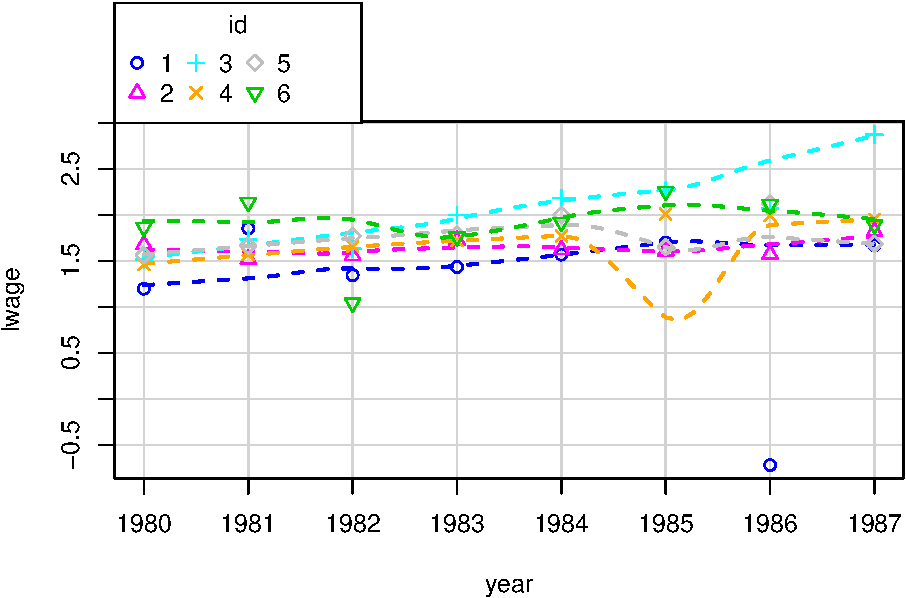
\includegraphics{09-paneldata_files/figure-latex/scatterplot chunk-1.pdf}

Для получения графиков на различных плитках можно использовать coplot.

\begin{Shaded}
\begin{Highlighting}[]
\KeywordTok{coplot}\NormalTok{(lwage }\OperatorTok{~}\StringTok{ }\NormalTok{year}\OperatorTok{|}\NormalTok{id, }\DataTypeTok{type =} \StringTok{'b'}\NormalTok{, }\DataTypeTok{data =}\NormalTok{ panel)}
\end{Highlighting}
\end{Shaded}

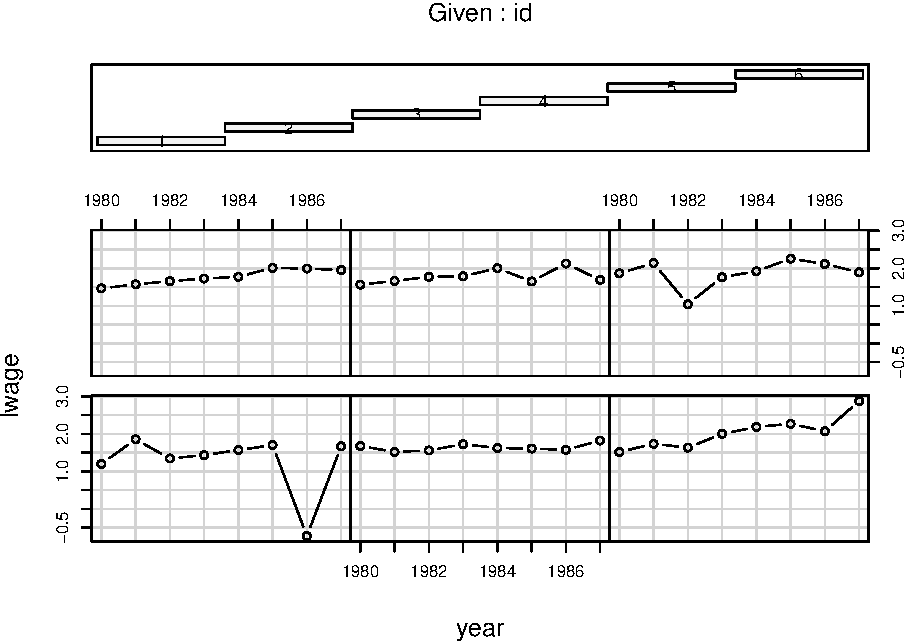
\includegraphics{09-paneldata_files/figure-latex/1 coplot chunk-1.pdf}

Сгруппировать можно по разным признакам. Например, в зависимости от расы индивидов.

\begin{Shaded}
\begin{Highlighting}[]
\NormalTok{panel}\OperatorTok{$}\NormalTok{year =}\StringTok{ }\KeywordTok{factor}\NormalTok{(panel}\OperatorTok{$}\NormalTok{year)}
\KeywordTok{coplot}\NormalTok{(lwage }\OperatorTok{~}\StringTok{ }\NormalTok{year}\OperatorTok{|}\NormalTok{black, }\DataTypeTok{type=}\StringTok{"l"}\NormalTok{, }\DataTypeTok{data=}\NormalTok{panel, }\DataTypeTok{panel =} \ControlFlowTok{function}\NormalTok{(x, y, ...) }\KeywordTok{panel.smooth}\NormalTok{(x, y, }\DataTypeTok{span =} \FloatTok{0.3}\NormalTok{, ...), }\DataTypeTok{pch =} \DecValTok{16}\NormalTok{, }\DataTypeTok{show.given =}\NormalTok{ F, }\DataTypeTok{xlab =} \StringTok{"Mean dependence lwage of year for white and black people"}\NormalTok{)}
\end{Highlighting}
\end{Shaded}

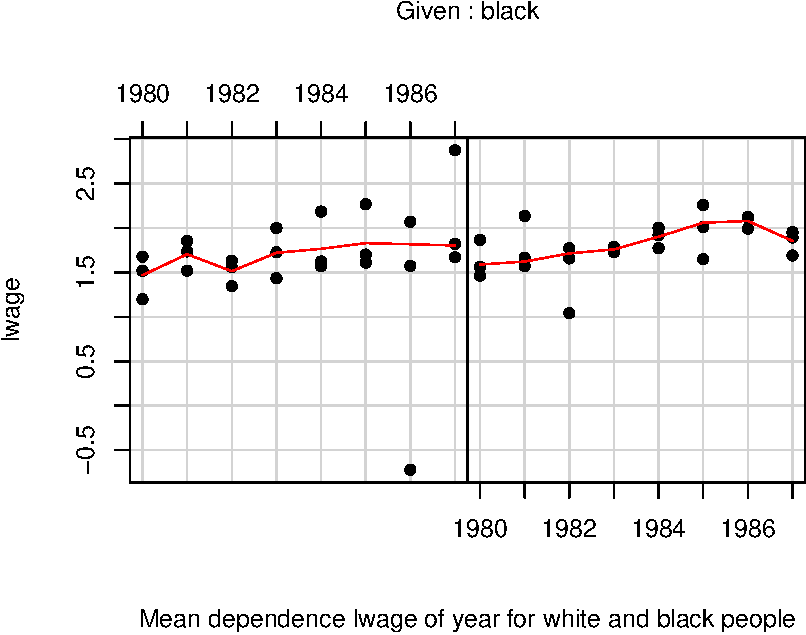
\includegraphics{09-paneldata_files/figure-latex/2 coplot chunk-1.pdf}

Импортируем основной датасет.

\begin{Shaded}
\begin{Highlighting}[]
\NormalTok{Panel =}\StringTok{ }\KeywordTok{import}\NormalTok{(}\StringTok{'lwage_panel_large.csv'}\NormalTok{)}
\end{Highlighting}
\end{Shaded}

Визуализируем гетерогенный эффект. Можно визуализировать по годам или по индивидам. Здесь уже можно использовать полный датасет. Так как доверительные интервалы с интервалом в год не пересекаются, можно увидеть явную гетерогенность.

\begin{Shaded}
\begin{Highlighting}[]
\KeywordTok{plotmeans}\NormalTok{(lwage }\OperatorTok{~}\StringTok{ }\NormalTok{year, }\DataTypeTok{main=}\StringTok{"Heterogeineity across years"}\NormalTok{, }\DataTypeTok{data=}\NormalTok{Panel)}
\end{Highlighting}
\end{Shaded}

\begin{verbatim}
Error in plotmeans(lwage ~ year, main = "Heterogeineity across years", : could not find function "plotmeans"
\end{verbatim}

Модель панельных данных будет выглядеть следующим образом:

\begin{equation}
y_{i t}=\alpha+x_{i t}^{\prime} \beta+z_{i}^{\prime} \gamma+c_{i}+u_{i t}
\end{equation}

где \(\alpha\) -- константа, \(c_{i}\) - индивидуальные эффекты индивидов, а \(z_i\) -- независимые от времени переменные. Следовательно, матрица \(X\) - матрица зависимых от времени регрессов, \(Z\) - матрица независимых от времени регрессоров. Дополнительно обозначим как \(l_n\) вектор из единиц.

Оценим простую модель с фиксированными эффектами через within-оценку. Вычитая \(\overline{y}_{i}=1 / T \sum_{t} y_{i t}\) из исходной модели, получим within-модель:

\begin{equation}
\ddot{y}_{i t}=\ddot{x}_{i t}^{\prime} \beta+\ddot{u}_{i t}
\end{equation}

где \(\ddot{y}_{i t}=y_{i t}-\overline{y}_{i}, \ddot{x}_{i t k}=x_{i t k}-\overline{x}_{i k}\) and \(\ddot{u}_{i t}=u_{i t}-\overline{u}_{i}\). Следует заметить, что константа \(\alpha\), индивидуальные эффекты \(c_i\) и инвариантные ко времени регрессоры \(z_i\) исчезают из модели.

\begin{equation}
\widehat{\beta}_{F E}=\left(\ddot{X}^{\prime} \ddot{X}\right)^{-1} \ddot{X}^{\prime} \ddot{y}
\end{equation}

\begin{Shaded}
\begin{Highlighting}[]
\NormalTok{ffe =}\StringTok{ }\KeywordTok{plm}\NormalTok{(lwage }\OperatorTok{~}\StringTok{ }\NormalTok{hours, }\DataTypeTok{model=}\StringTok{"within"}\NormalTok{, }\DataTypeTok{data =}\NormalTok{ Panel)}
\end{Highlighting}
\end{Shaded}

\begin{verbatim}
Error in plm(lwage ~ hours, model = "within", data = Panel): could not find function "plm"
\end{verbatim}

\begin{Shaded}
\begin{Highlighting}[]
\KeywordTok{summary}\NormalTok{(ffe)}
\end{Highlighting}
\end{Shaded}

\begin{verbatim}
Error in summary(ffe): object 'ffe' not found
\end{verbatim}

Проверим значимость коэффициентов, используя ковариационную матрицу ошибок Хубера - Уайта.

\begin{Shaded}
\begin{Highlighting}[]
\KeywordTok{coeftest}\NormalTok{(ffe, }\DataTypeTok{vcov=}\KeywordTok{vcovHC}\NormalTok{(ffe, }\DataTypeTok{cluster=}\StringTok{"group"}\NormalTok{))}
\end{Highlighting}
\end{Shaded}

\begin{verbatim}
Error in coeftest(ffe, vcov = vcovHC(ffe, cluster = "group")): object 'ffe' not found
\end{verbatim}

Оценим модель со случайными эффектами, используя достижимый обобщённый МНК (FGLS).

\begin{equation}
\left(\begin{array}{c}{\widehat{\alpha}_{R E}} \\ {\widehat{\beta}_{R E}} \\ {\widehat{\gamma}_{R E}}\end{array}\right)=\left(W^{\prime} \widehat{\Omega}_{v}^{-1} W\right)^{-1} W^{\prime} \widehat{\Omega}_{v}^{-1} y
\end{equation}

где

\(W=\left[\iota_{N T} X Z\right] \text { и } \iota_{N T} \text { это вектор из единиц размерности } N T \times 1\)

\begin{Shaded}
\begin{Highlighting}[]
\NormalTok{fre =}\StringTok{ }\KeywordTok{plm}\NormalTok{(lwage }\OperatorTok{~}\StringTok{ }\NormalTok{hours, }\DataTypeTok{model=}\StringTok{"random"}\NormalTok{, }\DataTypeTok{data =}\NormalTok{ Panel)}
\end{Highlighting}
\end{Shaded}

\begin{verbatim}
Error in plm(lwage ~ hours, model = "random", data = Panel): could not find function "plm"
\end{verbatim}

\begin{Shaded}
\begin{Highlighting}[]
\KeywordTok{summary}\NormalTok{(fre)}
\end{Highlighting}
\end{Shaded}

\begin{verbatim}
Error in summary(fre): object 'fre' not found
\end{verbatim}

Проверим значимость коэффициентов, используя ковариационную матрицу ошибок Хубера - Уайта.

\begin{Shaded}
\begin{Highlighting}[]
\KeywordTok{coeftest}\NormalTok{(fre, }\DataTypeTok{vcov=}\KeywordTok{vcovHC}\NormalTok{(ffe, }\DataTypeTok{cluster=}\StringTok{"group"}\NormalTok{))}
\end{Highlighting}
\end{Shaded}

\begin{verbatim}
Error in coeftest(fre, vcov = vcovHC(ffe, cluster = "group")): object 'fre' not found
\end{verbatim}

Проведём тест Хаусмана

\begin{Shaded}
\begin{Highlighting}[]
\KeywordTok{phtest}\NormalTok{(ffe, fre)}
\end{Highlighting}
\end{Shaded}

\begin{verbatim}
Error in phtest(ffe, fre): could not find function "phtest"
\end{verbatim}

Построим FD-оценку.

\begin{equation}
\dot{y}_{i t}=\dot{x}_{i t}^{\prime} \beta+\dot{u}_{i t}
\end{equation}

\(\dot{y}_{i t}=y_{i t}-y_{i, t-1}, \dot{x}_{i t}=x_{i t}-x_{i, t-1}\) и \(\dot{u}_{i t}=u_{i t}-u_{i, t-1}\)

\begin{Shaded}
\begin{Highlighting}[]
\NormalTok{fd =}\StringTok{ }\KeywordTok{plm}\NormalTok{(lwage }\OperatorTok{~}\StringTok{ }\NormalTok{hours }\OperatorTok{-}\StringTok{ }\DecValTok{1}\NormalTok{, }\DataTypeTok{model=}\StringTok{"fd"}\NormalTok{, }\DataTypeTok{data =}\NormalTok{ Panel)}
\end{Highlighting}
\end{Shaded}

\begin{verbatim}
Error in plm(lwage ~ hours - 1, model = "fd", data = Panel): could not find function "plm"
\end{verbatim}

\begin{Shaded}
\begin{Highlighting}[]
\KeywordTok{summary}\NormalTok{(fd)}
\end{Highlighting}
\end{Shaded}

\begin{verbatim}
Error in summary(fd): object 'fd' not found
\end{verbatim}

Построим LS-оценку с дамми-переменными по каждому индивиду (LSDV). Видим, что численно её результаты идентичны withih-регрессии, как и должно быть.

\begin{Shaded}
\begin{Highlighting}[]
\NormalTok{lsdv =}\StringTok{ }\KeywordTok{lm}\NormalTok{(lwage }\OperatorTok{~}\StringTok{ }\NormalTok{hours }\OperatorTok{+}\StringTok{ }\KeywordTok{factor}\NormalTok{(id) }\OperatorTok{-}\StringTok{ }\DecValTok{1}\NormalTok{, }\DataTypeTok{data=}\NormalTok{Panel)}
\KeywordTok{summary}\NormalTok{(lsdv)}
\end{Highlighting}
\end{Shaded}

\begin{verbatim}

Call:
lm(formula = lwage ~ hours + factor(id) - 1, data = Panel)

Residuals:
    Min      1Q  Median      3Q     Max 
-4.1161 -0.1370  0.0158  0.1825  1.5551 

Coefficients:
                Estimate Std. Error t value Pr(>|t|)    
hours         -5.585e-07  1.401e-05  -0.040 0.968208    
factor(id)1    1.257e+00  1.425e-01   8.825  < 2e-16 ***
factor(id)2    1.639e+00  1.413e-01  11.597  < 2e-16 ***
factor(id)3    2.036e+00  1.408e-01  14.455  < 2e-16 ***
factor(id)4    1.775e+00  1.404e-01  12.639  < 2e-16 ***
factor(id)5    2.056e+00  1.401e-01  14.680  < 2e-16 ***
factor(id)6    1.435e+00  1.424e-01  10.076  < 2e-16 ***
factor(id)7    1.996e+00  1.418e-01  14.077  < 2e-16 ***
factor(id)8    1.065e+00  1.434e-01   7.426 1.37e-13 ***
factor(id)9    1.474e+00  1.398e-01  10.537  < 2e-16 ***
factor(id)10   1.395e+00  1.394e-01  10.005  < 2e-16 ***
factor(id)11   1.385e+00  1.378e-01  10.052  < 2e-16 ***
factor(id)12   2.193e+00  1.396e-01  15.711  < 2e-16 ***
factor(id)13   1.840e+00  1.404e-01  13.103  < 2e-16 ***
factor(id)14   2.060e+00  1.413e-01  14.581  < 2e-16 ***
factor(id)15   2.455e+00  1.405e-01  17.468  < 2e-16 ***
factor(id)16   1.675e+00  1.400e-01  11.963  < 2e-16 ***
factor(id)17   1.697e+00  1.411e-01  12.031  < 2e-16 ***
factor(id)18   2.033e+00  1.398e-01  14.544  < 2e-16 ***
factor(id)19   2.214e+00  1.425e-01  15.533  < 2e-16 ***
factor(id)20   1.525e+00  1.400e-01  10.896  < 2e-16 ***
factor(id)21   1.726e+00  1.401e-01  12.321  < 2e-16 ***
factor(id)22   1.769e+00  1.400e-01  12.635  < 2e-16 ***
factor(id)23   2.077e+00  1.408e-01  14.754  < 2e-16 ***
factor(id)24   2.368e+00  1.400e-01  16.919  < 2e-16 ***
factor(id)25   1.311e+00  1.443e-01   9.085  < 2e-16 ***
factor(id)26   1.700e+00  1.399e-01  12.153  < 2e-16 ***
factor(id)27   2.284e+00  1.409e-01  16.214  < 2e-16 ***
factor(id)28   1.411e+00  1.411e-01  10.000  < 2e-16 ***
factor(id)29   7.640e-01  1.412e-01   5.409 6.71e-08 ***
factor(id)30   1.950e+00  1.403e-01  13.895  < 2e-16 ***
factor(id)31   1.670e+00  1.402e-01  11.917  < 2e-16 ***
factor(id)32   1.928e+00  1.407e-01  13.709  < 2e-16 ***
factor(id)33   2.362e+00  1.396e-01  16.918  < 2e-16 ***
factor(id)34   1.098e+00  1.409e-01   7.791 8.49e-15 ***
factor(id)35   2.103e+00  1.402e-01  14.995  < 2e-16 ***
factor(id)36   1.657e+00  1.402e-01  11.816  < 2e-16 ***
factor(id)37   1.664e+00  1.416e-01  11.753  < 2e-16 ***
factor(id)38   1.694e+00  1.406e-01  12.045  < 2e-16 ***
factor(id)39   2.063e+00  1.416e-01  14.576  < 2e-16 ***
factor(id)40   1.657e+00  1.400e-01  11.833  < 2e-16 ***
factor(id)41   5.381e-01  1.386e-01   3.883 0.000105 ***
factor(id)42   7.392e-01  1.390e-01   5.319 1.10e-07 ***
factor(id)43   1.713e+00  1.388e-01  12.345  < 2e-16 ***
factor(id)44   1.782e+00  1.408e-01  12.660  < 2e-16 ***
factor(id)45   1.989e+00  1.399e-01  14.215  < 2e-16 ***
factor(id)46   1.763e+00  1.413e-01  12.476  < 2e-16 ***
factor(id)47   1.128e+00  1.393e-01   8.095 7.63e-16 ***
factor(id)48   2.019e+00  1.416e-01  14.260  < 2e-16 ***
factor(id)49   8.453e-01  1.383e-01   6.112 1.08e-09 ***
factor(id)50   1.874e+00  1.409e-01  13.301  < 2e-16 ***
factor(id)51   1.759e+00  1.391e-01  12.644  < 2e-16 ***
factor(id)52   1.487e+00  1.397e-01  10.648  < 2e-16 ***
factor(id)53   2.212e+00  1.413e-01  15.658  < 2e-16 ***
factor(id)54   1.182e+00  1.391e-01   8.494  < 2e-16 ***
factor(id)55   2.022e+00  1.403e-01  14.411  < 2e-16 ***
factor(id)56   1.301e+00  1.390e-01   9.354  < 2e-16 ***
factor(id)57   1.353e+00  1.420e-01   9.525  < 2e-16 ***
factor(id)58   2.352e+00  1.406e-01  16.729  < 2e-16 ***
factor(id)59   2.146e+00  1.398e-01  15.346  < 2e-16 ***
factor(id)60   1.435e+00  1.400e-01  10.249  < 2e-16 ***
factor(id)61   1.250e+00  1.436e-01   8.703  < 2e-16 ***
factor(id)62   2.068e+00  1.402e-01  14.756  < 2e-16 ***
factor(id)63   1.305e+00  1.410e-01   9.257  < 2e-16 ***
factor(id)64   1.965e+00  1.404e-01  13.994  < 2e-16 ***
factor(id)65   1.374e+00  1.395e-01   9.852  < 2e-16 ***
factor(id)66   1.379e+00  1.421e-01   9.704  < 2e-16 ***
factor(id)67   1.181e+00  1.415e-01   8.346  < 2e-16 ***
factor(id)68   1.779e+00  1.401e-01  12.702  < 2e-16 ***
factor(id)69   1.157e+00  1.439e-01   8.040 1.19e-15 ***
factor(id)70   2.089e+00  1.387e-01  15.058  < 2e-16 ***
factor(id)71   2.081e+00  1.403e-01  14.829  < 2e-16 ***
factor(id)72   1.780e+00  1.400e-01  12.714  < 2e-16 ***
factor(id)73   1.927e+00  1.405e-01  13.716  < 2e-16 ***
factor(id)74   1.546e+00  1.395e-01  11.084  < 2e-16 ***
factor(id)75   1.874e+00  1.402e-01  13.369  < 2e-16 ***
factor(id)76   1.319e+00  1.397e-01   9.444  < 2e-16 ***
factor(id)77   1.935e+00  1.400e-01  13.819  < 2e-16 ***
factor(id)78   1.469e+00  1.420e-01  10.343  < 2e-16 ***
factor(id)79   1.782e+00  1.393e-01  12.792  < 2e-16 ***
factor(id)80   1.677e+00  1.484e-01  11.304  < 2e-16 ***
factor(id)81   2.016e+00  1.399e-01  14.405  < 2e-16 ***
factor(id)82   1.291e+00  1.407e-01   9.175  < 2e-16 ***
factor(id)83   1.650e+00  1.410e-01  11.707  < 2e-16 ***
factor(id)84   1.710e+00  1.400e-01  12.214  < 2e-16 ***
factor(id)85   1.194e+00  1.413e-01   8.452  < 2e-16 ***
factor(id)86   1.491e+00  1.399e-01  10.661  < 2e-16 ***
factor(id)87   1.049e+00  1.426e-01   7.354 2.35e-13 ***
factor(id)88   1.215e+00  1.401e-01   8.669  < 2e-16 ***
factor(id)89   1.492e+00  1.406e-01  10.612  < 2e-16 ***
factor(id)90   1.429e+00  1.413e-01  10.115  < 2e-16 ***
factor(id)91   1.206e+00  1.396e-01   8.640  < 2e-16 ***
factor(id)92   1.558e+00  1.406e-01  11.082  < 2e-16 ***
factor(id)93   1.751e+00  1.422e-01  12.312  < 2e-16 ***
factor(id)94   1.728e+00  1.402e-01  12.327  < 2e-16 ***
factor(id)95   1.573e+00  1.398e-01  11.250  < 2e-16 ***
factor(id)96   2.075e+00  1.401e-01  14.812  < 2e-16 ***
factor(id)97   1.526e+00  1.400e-01  10.897  < 2e-16 ***
factor(id)98   1.874e+00  1.407e-01  13.318  < 2e-16 ***
factor(id)99   1.741e+00  1.396e-01  12.472  < 2e-16 ***
factor(id)100  2.157e+00  1.400e-01  15.408  < 2e-16 ***
factor(id)101  2.087e+00  1.402e-01  14.887  < 2e-16 ***
factor(id)102  1.832e+00  1.390e-01  13.178  < 2e-16 ***
factor(id)103  1.072e+00  1.386e-01   7.736 1.31e-14 ***
factor(id)104  1.393e+00  1.408e-01   9.898  < 2e-16 ***
factor(id)105  2.552e+00  1.401e-01  18.215  < 2e-16 ***
factor(id)106  1.115e+00  1.396e-01   7.989 1.78e-15 ***
factor(id)107  1.900e+00  1.402e-01  13.545  < 2e-16 ***
factor(id)108  1.339e+00  1.400e-01   9.565  < 2e-16 ***
factor(id)109  1.707e+00  1.410e-01  12.101  < 2e-16 ***
factor(id)110  1.452e+00  1.387e-01  10.469  < 2e-16 ***
factor(id)111  1.853e+00  1.417e-01  13.073  < 2e-16 ***
factor(id)112  1.700e+00  1.421e-01  11.964  < 2e-16 ***
factor(id)113  1.997e+00  1.394e-01  14.327  < 2e-16 ***
factor(id)114  1.143e+00  1.402e-01   8.152 4.79e-16 ***
factor(id)115  1.835e+00  1.418e-01  12.945  < 2e-16 ***
factor(id)116  1.515e+00  1.397e-01  10.847  < 2e-16 ***
factor(id)117  1.679e+00  1.443e-01  11.635  < 2e-16 ***
factor(id)118  1.374e+00  1.379e-01   9.969  < 2e-16 ***
factor(id)119  1.982e+00  1.402e-01  14.130  < 2e-16 ***
factor(id)120  2.333e+00  1.403e-01  16.626  < 2e-16 ***
factor(id)121  1.764e+00  1.398e-01  12.620  < 2e-16 ***
factor(id)122  1.698e+00  1.394e-01  12.180  < 2e-16 ***
factor(id)123  2.116e+00  1.409e-01  15.022  < 2e-16 ***
factor(id)124  3.344e-01  1.394e-01   2.398 0.016514 *  
factor(id)125  1.083e+00  1.414e-01   7.658 2.37e-14 ***
factor(id)126  2.279e+00  1.400e-01  16.280  < 2e-16 ***
factor(id)127  1.372e+00  1.400e-01   9.804  < 2e-16 ***
factor(id)128  1.629e+00  1.398e-01  11.650  < 2e-16 ***
factor(id)129  1.669e+00  1.409e-01  11.845  < 2e-16 ***
factor(id)130  1.826e+00  1.423e-01  12.831  < 2e-16 ***
factor(id)131  2.243e+00  1.405e-01  15.960  < 2e-16 ***
factor(id)132  1.448e+00  1.399e-01  10.349  < 2e-16 ***
factor(id)133  1.154e+00  1.396e-01   8.261  < 2e-16 ***
factor(id)134  1.131e+00  1.392e-01   8.125 5.97e-16 ***
factor(id)135  2.035e+00  1.405e-01  14.485  < 2e-16 ***
factor(id)136  2.016e+00  1.405e-01  14.348  < 2e-16 ***
factor(id)137  1.839e+00  1.401e-01  13.131  < 2e-16 ***
factor(id)138  1.489e+00  1.399e-01  10.644  < 2e-16 ***
factor(id)139  1.736e+00  1.399e-01  12.413  < 2e-16 ***
factor(id)140  1.241e+00  1.390e-01   8.926  < 2e-16 ***
factor(id)141  1.067e+00  1.392e-01   7.668 2.21e-14 ***
factor(id)142  1.717e+00  1.404e-01  12.227  < 2e-16 ***
factor(id)143  2.174e+00  1.403e-01  15.494  < 2e-16 ***
factor(id)144  1.199e+00  1.455e-01   8.241 2.32e-16 ***
factor(id)145  1.574e+00  1.409e-01  11.171  < 2e-16 ***
factor(id)146  1.834e+00  1.411e-01  12.991  < 2e-16 ***
factor(id)147  1.319e+00  1.400e-01   9.422  < 2e-16 ***
factor(id)148  2.021e+00  1.401e-01  14.424  < 2e-16 ***
factor(id)149  1.622e+00  1.403e-01  11.567  < 2e-16 ***
factor(id)150  1.163e+00  1.407e-01   8.270  < 2e-16 ***
factor(id)151  2.226e+00  1.400e-01  15.900  < 2e-16 ***
factor(id)152  1.304e+00  1.416e-01   9.208  < 2e-16 ***
factor(id)153  2.283e+00  1.402e-01  16.290  < 2e-16 ***
factor(id)154  1.108e+00  1.403e-01   7.893 3.83e-15 ***
factor(id)155  9.691e-01  1.413e-01   6.860 8.00e-12 ***
factor(id)156  1.453e+00  1.400e-01  10.378  < 2e-16 ***
factor(id)157  1.716e+00  1.398e-01  12.279  < 2e-16 ***
factor(id)158  1.617e+00  1.405e-01  11.510  < 2e-16 ***
factor(id)159  2.082e+00  1.392e-01  14.963  < 2e-16 ***
factor(id)160  1.294e+00  1.400e-01   9.241  < 2e-16 ***
factor(id)161  1.464e+00  1.401e-01  10.445  < 2e-16 ***
factor(id)162  1.863e+00  1.407e-01  13.247  < 2e-16 ***
factor(id)163  1.778e+00  1.399e-01  12.708  < 2e-16 ***
factor(id)164  2.002e+00  1.396e-01  14.341  < 2e-16 ***
factor(id)165  1.891e+00  1.422e-01  13.297  < 2e-16 ***
factor(id)166  2.150e+00  1.395e-01  15.414  < 2e-16 ***
factor(id)167  1.067e+00  1.392e-01   7.662 2.31e-14 ***
factor(id)168  1.539e+00  1.387e-01  11.100  < 2e-16 ***
factor(id)169  1.196e+00  1.400e-01   8.548  < 2e-16 ***
factor(id)170  1.568e+00  1.395e-01  11.244  < 2e-16 ***
factor(id)171  1.674e+00  1.426e-01  11.740  < 2e-16 ***
factor(id)172  1.751e+00  1.411e-01  12.407  < 2e-16 ***
factor(id)173  2.264e+00  1.408e-01  16.077  < 2e-16 ***
factor(id)174  2.221e+00  1.402e-01  15.842  < 2e-16 ***
factor(id)175  1.775e+00  1.414e-01  12.547  < 2e-16 ***
factor(id)176  2.361e+00  1.400e-01  16.867  < 2e-16 ***
factor(id)177  1.784e+00  1.407e-01  12.680  < 2e-16 ***
factor(id)178  9.877e-01  1.407e-01   7.018 2.66e-12 ***
factor(id)179  7.941e-01  1.395e-01   5.691 1.36e-08 ***
factor(id)180  1.910e+00  1.400e-01  13.646  < 2e-16 ***
factor(id)181  2.093e+00  1.398e-01  14.972  < 2e-16 ***
factor(id)182  1.775e+00  1.393e-01  12.741  < 2e-16 ***
factor(id)183  2.011e+00  1.406e-01  14.302  < 2e-16 ***
factor(id)184  1.898e+00  1.398e-01  13.575  < 2e-16 ***
factor(id)185  1.884e+00  1.410e-01  13.361  < 2e-16 ***
factor(id)186  1.606e+00  1.392e-01  11.537  < 2e-16 ***
factor(id)187  1.841e+00  1.401e-01  13.143  < 2e-16 ***
factor(id)188  1.578e+00  1.405e-01  11.230  < 2e-16 ***
factor(id)189  2.079e+00  1.402e-01  14.825  < 2e-16 ***
factor(id)190  1.963e+00  1.386e-01  14.161  < 2e-16 ***
factor(id)191  1.444e+00  1.392e-01  10.373  < 2e-16 ***
factor(id)192  1.462e+00  1.400e-01  10.438  < 2e-16 ***
factor(id)193  1.786e+00  1.386e-01  12.892  < 2e-16 ***
factor(id)194  1.390e+00  1.409e-01   9.864  < 2e-16 ***
factor(id)195  8.809e-01  1.375e-01   6.406 1.68e-10 ***
factor(id)196  1.660e+00  1.403e-01  11.831  < 2e-16 ***
factor(id)197  1.788e+00  1.386e-01  12.904  < 2e-16 ***
factor(id)198  1.813e+00  1.393e-01  13.015  < 2e-16 ***
factor(id)199  1.740e+00  1.399e-01  12.436  < 2e-16 ***
factor(id)200  1.730e+00  1.393e-01  12.424  < 2e-16 ***
factor(id)201  2.524e+00  1.395e-01  18.096  < 2e-16 ***
factor(id)202  1.174e+00  1.393e-01   8.432  < 2e-16 ***
factor(id)203  1.215e+00  1.393e-01   8.726  < 2e-16 ***
factor(id)204  1.746e+00  1.411e-01  12.378  < 2e-16 ***
factor(id)205  1.806e+00  1.406e-01  12.839  < 2e-16 ***
factor(id)206  1.829e+00  1.419e-01  12.888  < 2e-16 ***
factor(id)207  1.874e+00  1.398e-01  13.401  < 2e-16 ***
factor(id)208  1.621e+00  1.405e-01  11.539  < 2e-16 ***
factor(id)209  1.965e+00  1.407e-01  13.968  < 2e-16 ***
factor(id)210  1.496e+00  1.395e-01  10.719  < 2e-16 ***
factor(id)211  1.063e+00  1.395e-01   7.623 3.12e-14 ***
factor(id)212  1.906e+00  1.406e-01  13.558  < 2e-16 ***
factor(id)213  1.442e+00  1.402e-01  10.284  < 2e-16 ***
factor(id)214  2.195e+00  1.404e-01  15.638  < 2e-16 ***
factor(id)215  1.597e+00  1.398e-01  11.425  < 2e-16 ***
factor(id)216  2.107e+00  1.400e-01  15.050  < 2e-16 ***
factor(id)217  2.296e+00  1.382e-01  16.612  < 2e-16 ***
factor(id)218  1.735e+00  1.399e-01  12.400  < 2e-16 ***
factor(id)219  2.044e+00  1.399e-01  14.608  < 2e-16 ***
factor(id)220  1.842e+00  1.399e-01  13.167  < 2e-16 ***
factor(id)221  2.098e+00  1.400e-01  14.987  < 2e-16 ***
factor(id)222  1.562e+00  1.399e-01  11.162  < 2e-16 ***
factor(id)223  1.889e+00  1.390e-01  13.597  < 2e-16 ***
factor(id)224  1.609e+00  1.411e-01  11.405  < 2e-16 ***
factor(id)225  1.953e+00  1.403e-01  13.917  < 2e-16 ***
factor(id)226  2.024e+00  1.412e-01  14.331  < 2e-16 ***
factor(id)227  2.148e+00  1.406e-01  15.282  < 2e-16 ***
factor(id)228  7.610e-01  1.389e-01   5.478 4.57e-08 ***
factor(id)229  1.648e+00  1.401e-01  11.765  < 2e-16 ***
factor(id)230  2.164e+00  1.424e-01  15.196  < 2e-16 ***
factor(id)231  1.953e+00  1.410e-01  13.854  < 2e-16 ***
factor(id)232  1.717e+00  1.404e-01  12.229  < 2e-16 ***
factor(id)233  1.791e+00  1.400e-01  12.799  < 2e-16 ***
factor(id)234  1.924e+00  1.408e-01  13.665  < 2e-16 ***
factor(id)235  1.877e+00  1.398e-01  13.423  < 2e-16 ***
factor(id)236  2.054e+00  1.402e-01  14.649  < 2e-16 ***
factor(id)237  1.377e+00  1.398e-01   9.851  < 2e-16 ***
factor(id)238  1.642e+00  1.405e-01  11.686  < 2e-16 ***
factor(id)239  2.352e+00  1.396e-01  16.854  < 2e-16 ***
factor(id)240  1.858e+00  1.403e-01  13.241  < 2e-16 ***
factor(id)241  1.303e+00  1.391e-01   9.368  < 2e-16 ***
factor(id)242  1.721e+00  1.422e-01  12.104  < 2e-16 ***
factor(id)243  1.643e+00  1.402e-01  11.713  < 2e-16 ***
factor(id)244  2.042e+00  1.400e-01  14.583  < 2e-16 ***
factor(id)245  1.352e+00  1.398e-01   9.667  < 2e-16 ***
factor(id)246  1.419e+00  1.413e-01  10.046  < 2e-16 ***
factor(id)247  1.495e+00  1.424e-01  10.497  < 2e-16 ***
factor(id)248  2.519e+00  1.403e-01  17.953  < 2e-16 ***
factor(id)249  2.531e+00  1.399e-01  18.087  < 2e-16 ***
factor(id)250  2.048e+00  1.400e-01  14.625  < 2e-16 ***
factor(id)251  1.288e+00  1.394e-01   9.241  < 2e-16 ***
factor(id)252  1.428e+00  1.407e-01  10.146  < 2e-16 ***
factor(id)253  1.873e+00  1.402e-01  13.362  < 2e-16 ***
factor(id)254  1.410e+00  1.402e-01  10.056  < 2e-16 ***
factor(id)255  1.509e+00  1.418e-01  10.643  < 2e-16 ***
factor(id)256  1.993e+00  1.403e-01  14.209  < 2e-16 ***
factor(id)257  1.911e+00  1.396e-01  13.689  < 2e-16 ***
factor(id)258  1.184e+00  1.415e-01   8.367  < 2e-16 ***
factor(id)259  1.773e+00  1.404e-01  12.632  < 2e-16 ***
factor(id)260  1.772e+00  1.427e-01  12.417  < 2e-16 ***
factor(id)261  1.071e+00  1.380e-01   7.758 1.10e-14 ***
factor(id)262  1.814e+00  1.404e-01  12.920  < 2e-16 ***
factor(id)263  1.300e+00  1.401e-01   9.278  < 2e-16 ***
factor(id)264  8.232e-01  1.385e-01   5.945 3.00e-09 ***
factor(id)265  1.521e+00  1.399e-01  10.873  < 2e-16 ***
factor(id)266  1.735e+00  1.395e-01  12.434  < 2e-16 ***
factor(id)267  1.191e+00  1.401e-01   8.501  < 2e-16 ***
factor(id)268  2.020e+00  1.408e-01  14.341  < 2e-16 ***
factor(id)269  1.939e+00  1.393e-01  13.917  < 2e-16 ***
factor(id)270  1.853e+00  1.390e-01  13.332  < 2e-16 ***
factor(id)271  1.393e+00  1.407e-01   9.899  < 2e-16 ***
factor(id)272  1.303e+00  1.402e-01   9.297  < 2e-16 ***
factor(id)273  2.135e+00  1.395e-01  15.303  < 2e-16 ***
factor(id)274  2.009e+00  1.397e-01  14.385  < 2e-16 ***
factor(id)275  1.382e+00  1.384e-01   9.988  < 2e-16 ***
factor(id)276  1.666e+00  1.416e-01  11.764  < 2e-16 ***
factor(id)277  1.320e+00  1.401e-01   9.420  < 2e-16 ***
factor(id)278  2.165e+00  1.400e-01  15.461  < 2e-16 ***
factor(id)279  1.372e+00  1.408e-01   9.739  < 2e-16 ***
factor(id)280  2.221e+00  1.400e-01  15.865  < 2e-16 ***
factor(id)281  1.767e+00  1.401e-01  12.611  < 2e-16 ***
factor(id)282  1.782e+00  1.414e-01  12.605  < 2e-16 ***
factor(id)283  1.311e+00  1.405e-01   9.333  < 2e-16 ***
factor(id)284  1.324e+00  1.402e-01   9.445  < 2e-16 ***
factor(id)285  1.051e+00  1.384e-01   7.598 3.75e-14 ***
factor(id)286  2.216e+00  1.398e-01  15.852  < 2e-16 ***
factor(id)287  1.226e+00  1.391e-01   8.816  < 2e-16 ***
factor(id)288  2.122e+00  1.400e-01  15.159  < 2e-16 ***
factor(id)289  1.599e+00  1.402e-01  11.407  < 2e-16 ***
factor(id)290  1.647e+00  1.403e-01  11.737  < 2e-16 ***
factor(id)291  1.373e+00  1.431e-01   9.594  < 2e-16 ***
factor(id)292  1.399e+00  1.400e-01   9.996  < 2e-16 ***
factor(id)293  1.120e+00  1.406e-01   7.965 2.17e-15 ***
factor(id)294  1.582e+00  1.409e-01  11.222  < 2e-16 ***
factor(id)295  1.179e+00  1.394e-01   8.456  < 2e-16 ***
factor(id)296  2.352e+00  1.403e-01  16.762  < 2e-16 ***
factor(id)297  2.279e+00  1.402e-01  16.257  < 2e-16 ***
factor(id)298  1.466e+00  1.433e-01  10.229  < 2e-16 ***
factor(id)299  1.836e+00  1.409e-01  13.033  < 2e-16 ***
factor(id)300  1.953e+00  1.407e-01  13.882  < 2e-16 ***
factor(id)301  2.216e+00  1.409e-01  15.728  < 2e-16 ***
factor(id)302  1.850e+00  1.399e-01  13.224  < 2e-16 ***
factor(id)303  1.739e+00  1.398e-01  12.446  < 2e-16 ***
factor(id)304  1.619e+00  1.414e-01  11.450  < 2e-16 ***
factor(id)305  1.650e+00  1.402e-01  11.768  < 2e-16 ***
factor(id)306  1.390e+00  1.415e-01   9.825  < 2e-16 ***
factor(id)307  1.322e+00  1.417e-01   9.329  < 2e-16 ***
factor(id)308  1.667e+00  1.404e-01  11.877  < 2e-16 ***
factor(id)309  2.002e+00  1.413e-01  14.169  < 2e-16 ***
factor(id)310  1.502e+00  1.416e-01  10.609  < 2e-16 ***
factor(id)311  1.434e+00  1.401e-01  10.232  < 2e-16 ***
factor(id)312  9.779e-01  1.396e-01   7.005 2.90e-12 ***
factor(id)313  1.342e+00  1.400e-01   9.584  < 2e-16 ***
factor(id)314  1.577e+00  1.397e-01  11.291  < 2e-16 ***
factor(id)315  1.530e+00  1.418e-01  10.784  < 2e-16 ***
factor(id)316  1.352e+00  1.395e-01   9.688  < 2e-16 ***
factor(id)317  1.258e+00  1.409e-01   8.925  < 2e-16 ***
factor(id)318  1.507e+00  1.413e-01  10.664  < 2e-16 ***
factor(id)319  1.437e+00  1.418e-01  10.133  < 2e-16 ***
factor(id)320  1.315e+00  1.406e-01   9.352  < 2e-16 ***
factor(id)321  1.680e+00  1.398e-01  12.014  < 2e-16 ***
factor(id)322  1.927e+00  1.414e-01  13.630  < 2e-16 ***
factor(id)323  1.447e+00  1.397e-01  10.358  < 2e-16 ***
factor(id)324  1.653e+00  1.420e-01  11.644  < 2e-16 ***
factor(id)325  1.805e+00  1.397e-01  12.921  < 2e-16 ***
factor(id)326  1.572e+00  1.401e-01  11.218  < 2e-16 ***
factor(id)327  1.948e+00  1.410e-01  13.818  < 2e-16 ***
factor(id)328  1.317e+00  1.409e-01   9.350  < 2e-16 ***
factor(id)329  1.777e+00  1.403e-01  12.663  < 2e-16 ***
factor(id)330  1.847e+00  1.397e-01  13.224  < 2e-16 ***
factor(id)331  1.914e+00  1.396e-01  13.709  < 2e-16 ***
factor(id)332  1.518e+00  1.400e-01  10.842  < 2e-16 ***
factor(id)333  1.725e+00  1.400e-01  12.320  < 2e-16 ***
factor(id)334  1.673e+00  1.399e-01  11.956  < 2e-16 ***
factor(id)335  1.233e+00  1.424e-01   8.661  < 2e-16 ***
factor(id)336  1.373e+00  1.402e-01   9.793  < 2e-16 ***
factor(id)337  1.249e+00  1.406e-01   8.888  < 2e-16 ***
factor(id)338  1.307e+00  1.391e-01   9.399  < 2e-16 ***
factor(id)339  1.633e+00  1.406e-01  11.615  < 2e-16 ***
factor(id)340  1.669e+00  1.397e-01  11.942  < 2e-16 ***
factor(id)341  1.989e+00  1.400e-01  14.209  < 2e-16 ***
factor(id)342  7.782e-01  1.417e-01   5.492 4.24e-08 ***
factor(id)343  7.649e-01  1.399e-01   5.466 4.89e-08 ***
factor(id)344  1.091e+00  1.401e-01   7.782 9.09e-15 ***
factor(id)345  1.593e+00  1.429e-01  11.149  < 2e-16 ***
factor(id)346  1.717e+00  1.401e-01  12.250  < 2e-16 ***
factor(id)347  1.800e+00  1.401e-01  12.846  < 2e-16 ***
factor(id)348  1.450e+00  1.395e-01  10.400  < 2e-16 ***
factor(id)349  1.851e+00  1.402e-01  13.208  < 2e-16 ***
factor(id)350  1.161e+00  1.392e-01   8.345  < 2e-16 ***
factor(id)351  2.047e+00  1.399e-01  14.632  < 2e-16 ***
factor(id)352  1.816e+00  1.406e-01  12.923  < 2e-16 ***
factor(id)353  2.172e+00  1.409e-01  15.414  < 2e-16 ***
factor(id)354  1.244e+00  1.398e-01   8.896  < 2e-16 ***
factor(id)355  2.019e+00  1.401e-01  14.415  < 2e-16 ***
factor(id)356  1.467e+00  1.400e-01  10.476  < 2e-16 ***
factor(id)357  1.600e+00  1.400e-01  11.430  < 2e-16 ***
factor(id)358  1.302e+00  1.415e-01   9.202  < 2e-16 ***
factor(id)359  1.698e+00  1.408e-01  12.057  < 2e-16 ***
factor(id)360  1.807e+00  1.408e-01  12.832  < 2e-16 ***
factor(id)361  1.837e+00  1.451e-01  12.660  < 2e-16 ***
factor(id)362  1.482e+00  1.394e-01  10.630  < 2e-16 ***
factor(id)363  2.686e+00  1.407e-01  19.096  < 2e-16 ***
factor(id)364  2.075e+00  1.400e-01  14.817  < 2e-16 ***
factor(id)365  1.734e+00  1.400e-01  12.387  < 2e-16 ***
factor(id)366  1.715e+00  1.400e-01  12.248  < 2e-16 ***
factor(id)367  1.018e+00  1.395e-01   7.297 3.55e-13 ***
factor(id)368  1.391e+00  1.394e-01   9.979  < 2e-16 ***
factor(id)369  1.410e+00  1.400e-01  10.071  < 2e-16 ***
factor(id)370  1.409e+00  1.397e-01  10.081  < 2e-16 ***
factor(id)371  1.666e+00  1.410e-01  11.815  < 2e-16 ***
factor(id)372  1.219e+00  1.407e-01   8.665  < 2e-16 ***
factor(id)373  1.963e+00  1.396e-01  14.061  < 2e-16 ***
factor(id)374  1.415e+00  1.413e-01  10.013  < 2e-16 ***
factor(id)375  1.925e+00  1.403e-01  13.718  < 2e-16 ***
factor(id)376  1.605e+00  1.414e-01  11.358  < 2e-16 ***
factor(id)377  1.592e+00  1.422e-01  11.194  < 2e-16 ***
factor(id)378  1.783e+00  1.400e-01  12.734  < 2e-16 ***
factor(id)379  1.309e+00  1.440e-01   9.088  < 2e-16 ***
factor(id)380  1.897e+00  1.410e-01  13.452  < 2e-16 ***
factor(id)381  1.581e+00  1.387e-01  11.406  < 2e-16 ***
factor(id)382  3.175e+00  1.393e-01  22.796  < 2e-16 ***
factor(id)383  1.219e+00  1.389e-01   8.775  < 2e-16 ***
factor(id)384  1.769e+00  1.411e-01  12.532  < 2e-16 ***
factor(id)385  2.302e+00  1.405e-01  16.388  < 2e-16 ***
factor(id)386  1.732e+00  1.403e-01  12.346  < 2e-16 ***
factor(id)387  2.297e+00  1.400e-01  16.409  < 2e-16 ***
factor(id)388  1.802e+00  1.400e-01  12.867  < 2e-16 ***
factor(id)389  2.019e+00  1.410e-01  14.323  < 2e-16 ***
factor(id)390  1.593e+00  1.400e-01  11.381  < 2e-16 ***
factor(id)391  1.384e+00  1.401e-01   9.878  < 2e-16 ***
factor(id)392  2.439e+00  1.409e-01  17.310  < 2e-16 ***
factor(id)393  1.571e+00  1.402e-01  11.200  < 2e-16 ***
factor(id)394  1.505e+00  1.401e-01  10.745  < 2e-16 ***
factor(id)395  1.448e+00  1.402e-01  10.330  < 2e-16 ***
factor(id)396  1.377e+00  1.407e-01   9.783  < 2e-16 ***
factor(id)397  1.845e+00  1.402e-01  13.162  < 2e-16 ***
factor(id)398  1.497e+00  1.398e-01  10.710  < 2e-16 ***
factor(id)399  2.313e+00  1.408e-01  16.434  < 2e-16 ***
factor(id)400  1.224e+00  1.409e-01   8.690  < 2e-16 ***
factor(id)401  1.804e+00  1.416e-01  12.739  < 2e-16 ***
factor(id)402  2.198e+00  1.405e-01  15.648  < 2e-16 ***
factor(id)403  1.715e+00  1.400e-01  12.244  < 2e-16 ***
factor(id)404  1.699e+00  1.408e-01  12.069  < 2e-16 ***
factor(id)405  1.531e+00  1.397e-01  10.964  < 2e-16 ***
factor(id)406  2.051e+00  1.400e-01  14.650  < 2e-16 ***
factor(id)407  1.423e+00  1.411e-01  10.085  < 2e-16 ***
factor(id)408  1.456e+00  1.431e-01  10.177  < 2e-16 ***
factor(id)409  1.566e+00  1.400e-01  11.184  < 2e-16 ***
factor(id)410  1.326e+00  1.392e-01   9.530  < 2e-16 ***
factor(id)411  1.088e+00  1.393e-01   7.815 7.08e-15 ***
factor(id)412  9.472e-01  1.398e-01   6.774 1.45e-11 ***
factor(id)413  2.315e+00  1.398e-01  16.562  < 2e-16 ***
factor(id)414  8.820e-01  1.448e-01   6.092 1.23e-09 ***
factor(id)415  1.235e+00  1.398e-01   8.837  < 2e-16 ***
factor(id)416  1.254e+00  1.398e-01   8.968  < 2e-16 ***
factor(id)417  1.849e+00  1.403e-01  13.180  < 2e-16 ***
factor(id)418  1.394e+00  1.419e-01   9.825  < 2e-16 ***
factor(id)419  9.013e-01  1.407e-01   6.407 1.67e-10 ***
factor(id)420  1.391e+00  1.405e-01   9.900  < 2e-16 ***
factor(id)421  7.832e-01  1.400e-01   5.595 2.36e-08 ***
factor(id)422  1.735e+00  1.396e-01  12.430  < 2e-16 ***
factor(id)423  1.388e+00  1.412e-01   9.830  < 2e-16 ***
factor(id)424  1.697e+00  1.397e-01  12.146  < 2e-16 ***
factor(id)425  1.695e+00  1.430e-01  11.848  < 2e-16 ***
factor(id)426  1.529e+00  1.396e-01  10.948  < 2e-16 ***
factor(id)427  1.715e+00  1.411e-01  12.150  < 2e-16 ***
factor(id)428  2.054e+00  1.379e-01  14.897  < 2e-16 ***
factor(id)429  1.551e+00  1.401e-01  11.067  < 2e-16 ***
factor(id)430  1.369e+00  1.400e-01   9.777  < 2e-16 ***
factor(id)431  1.434e+00  1.403e-01  10.218  < 2e-16 ***
factor(id)432  1.238e+00  1.398e-01   8.853  < 2e-16 ***
factor(id)433  1.594e+00  1.402e-01  11.370  < 2e-16 ***
factor(id)434  2.363e+00  1.401e-01  16.866  < 2e-16 ***
factor(id)435  1.620e+00  1.402e-01  11.554  < 2e-16 ***
factor(id)436  9.913e-01  1.398e-01   7.091 1.58e-12 ***
factor(id)437  1.253e+00  1.426e-01   8.793  < 2e-16 ***
factor(id)438  1.066e+00  1.400e-01   7.615 3.29e-14 ***
factor(id)439  1.874e+00  1.439e-01  13.026  < 2e-16 ***
factor(id)440  2.082e+00  1.407e-01  14.789  < 2e-16 ***
factor(id)441  2.173e+00  1.400e-01  15.525  < 2e-16 ***
factor(id)442  1.622e+00  1.402e-01  11.572  < 2e-16 ***
factor(id)443  1.527e+00  1.444e-01  10.577  < 2e-16 ***
factor(id)444  2.185e+00  1.400e-01  15.602  < 2e-16 ***
factor(id)445  1.124e+00  1.429e-01   7.868 4.66e-15 ***
factor(id)446  1.357e+00  1.396e-01   9.721  < 2e-16 ***
factor(id)447  1.340e+00  1.404e-01   9.542  < 2e-16 ***
factor(id)448  1.545e+00  1.399e-01  11.045  < 2e-16 ***
factor(id)449  2.378e+00  1.396e-01  17.032  < 2e-16 ***
factor(id)450  1.193e+00  1.409e-01   8.463  < 2e-16 ***
factor(id)451  1.338e+00  1.439e-01   9.297  < 2e-16 ***
factor(id)452  1.425e+00  1.395e-01  10.214  < 2e-16 ***
factor(id)453  1.694e+00  1.402e-01  12.081  < 2e-16 ***
factor(id)454  1.402e+00  1.396e-01  10.046  < 2e-16 ***
factor(id)455  1.835e+00  1.407e-01  13.037  < 2e-16 ***
factor(id)456  1.503e+00  1.401e-01  10.730  < 2e-16 ***
factor(id)457  2.358e+00  1.407e-01  16.759  < 2e-16 ***
factor(id)458  2.015e+00  1.402e-01  14.369  < 2e-16 ***
factor(id)459  1.641e+00  1.395e-01  11.768  < 2e-16 ***
factor(id)460  1.551e+00  1.394e-01  11.124  < 2e-16 ***
factor(id)461  2.027e+00  1.402e-01  14.457  < 2e-16 ***
factor(id)462  1.757e+00  1.401e-01  12.547  < 2e-16 ***
factor(id)463  1.959e+00  1.406e-01  13.932  < 2e-16 ***
factor(id)464  1.024e+00  1.400e-01   7.311 3.20e-13 ***
factor(id)465  1.125e+00  1.406e-01   8.004 1.58e-15 ***
factor(id)466  1.627e+00  1.384e-01  11.761  < 2e-16 ***
factor(id)467  2.347e+00  1.396e-01  16.810  < 2e-16 ***
factor(id)468  1.161e+00  1.446e-01   8.030 1.29e-15 ***
factor(id)469  2.123e+00  1.397e-01  15.199  < 2e-16 ***
factor(id)470  1.340e+00  1.405e-01   9.538  < 2e-16 ***
factor(id)471  2.196e+00  1.382e-01  15.891  < 2e-16 ***
factor(id)472  1.569e+00  1.409e-01  11.134  < 2e-16 ***
factor(id)473  1.916e+00  1.407e-01  13.622  < 2e-16 ***
factor(id)474  2.626e+00  1.454e-01  18.065  < 2e-16 ***
factor(id)475  2.197e+00  1.402e-01  15.667  < 2e-16 ***
factor(id)476  1.859e+00  1.404e-01  13.244  < 2e-16 ***
factor(id)477  1.604e+00  1.421e-01  11.284  < 2e-16 ***
factor(id)478  1.707e+00  1.397e-01  12.217  < 2e-16 ***
factor(id)479  1.091e+00  1.464e-01   7.454 1.12e-13 ***
factor(id)480  2.014e+00  1.409e-01  14.297  < 2e-16 ***
factor(id)481  1.278e+00  1.408e-01   9.072  < 2e-16 ***
factor(id)482  1.245e+00  1.395e-01   8.929  < 2e-16 ***
factor(id)483  1.960e+00  1.429e-01  13.719  < 2e-16 ***
factor(id)484  1.972e+00  1.412e-01  13.967  < 2e-16 ***
factor(id)485  2.230e+00  1.402e-01  15.899  < 2e-16 ***
factor(id)486  1.769e+00  1.401e-01  12.630  < 2e-16 ***
factor(id)487  2.108e+00  1.406e-01  14.992  < 2e-16 ***
factor(id)488  1.473e+00  1.406e-01  10.476  < 2e-16 ***
factor(id)489  9.278e-01  1.414e-01   6.560 6.12e-11 ***
factor(id)490  1.740e+00  1.398e-01  12.443  < 2e-16 ***
factor(id)491  1.731e+00  1.411e-01  12.266  < 2e-16 ***
factor(id)492  1.089e+00  1.389e-01   7.835 6.05e-15 ***
factor(id)493  1.520e+00  1.403e-01  10.834  < 2e-16 ***
factor(id)494  1.707e+00  1.400e-01  12.195  < 2e-16 ***
factor(id)495  1.256e+00  1.401e-01   8.965  < 2e-16 ***
factor(id)496  1.730e+00  1.402e-01  12.343  < 2e-16 ***
factor(id)497  2.238e+00  1.402e-01  15.968  < 2e-16 ***
factor(id)498  1.575e+00  1.403e-01  11.225  < 2e-16 ***
factor(id)499  1.530e+00  1.409e-01  10.857  < 2e-16 ***
factor(id)500  1.168e+00  1.396e-01   8.370  < 2e-16 ***
factor(id)501  2.247e+00  1.423e-01  15.789  < 2e-16 ***
factor(id)502  1.389e+00  1.396e-01   9.949  < 2e-16 ***
factor(id)503  1.676e+00  1.391e-01  12.048  < 2e-16 ***
factor(id)504  1.600e+00  1.399e-01  11.436  < 2e-16 ***
factor(id)505  1.149e+00  1.420e-01   8.090 7.92e-16 ***
factor(id)506  9.673e-01  1.395e-01   6.932 4.84e-12 ***
factor(id)507  1.813e+00  1.407e-01  12.886  < 2e-16 ***
factor(id)508  4.152e-01  1.399e-01   2.968 0.003015 ** 
factor(id)509  1.254e+00  1.400e-01   8.956  < 2e-16 ***
factor(id)510  8.598e-01  1.392e-01   6.175 7.32e-10 ***
factor(id)511  1.279e+00  1.393e-01   9.178  < 2e-16 ***
factor(id)512  1.472e+00  1.383e-01  10.646  < 2e-16 ***
factor(id)513  1.579e+00  1.409e-01  11.205  < 2e-16 ***
factor(id)514  2.003e+00  1.404e-01  14.269  < 2e-16 ***
factor(id)515  2.164e+00  1.415e-01  15.294  < 2e-16 ***
factor(id)516  1.545e+00  1.374e-01  11.246  < 2e-16 ***
factor(id)517  1.546e+00  1.409e-01  10.975  < 2e-16 ***
factor(id)518  2.192e+00  1.397e-01  15.690  < 2e-16 ***
factor(id)519  1.562e+00  1.494e-01  10.453  < 2e-16 ***
factor(id)520  1.644e+00  1.428e-01  11.517  < 2e-16 ***
factor(id)521  1.094e+00  1.400e-01   7.819 6.85e-15 ***
factor(id)522  1.648e+00  1.406e-01  11.723  < 2e-16 ***
factor(id)523  2.240e+00  1.394e-01  16.072  < 2e-16 ***
factor(id)524  1.506e+00  1.408e-01  10.700  < 2e-16 ***
factor(id)525  1.773e+00  1.390e-01  12.755  < 2e-16 ***
factor(id)526  1.487e+00  1.382e-01  10.757  < 2e-16 ***
factor(id)527  1.856e+00  1.407e-01  13.190  < 2e-16 ***
factor(id)528  1.433e+00  1.391e-01  10.301  < 2e-16 ***
factor(id)529  1.311e+00  1.391e-01   9.427  < 2e-16 ***
factor(id)530  1.174e+00  1.423e-01   8.251  < 2e-16 ***
factor(id)531  1.493e+00  1.389e-01  10.752  < 2e-16 ***
factor(id)532  1.839e+00  1.393e-01  13.204  < 2e-16 ***
factor(id)533  1.969e+00  1.405e-01  14.013  < 2e-16 ***
factor(id)534  7.982e-01  1.402e-01   5.694 1.33e-08 ***
factor(id)535  1.137e+00  1.414e-01   8.042 1.17e-15 ***
factor(id)536  1.715e+00  1.408e-01  12.181  < 2e-16 ***
factor(id)537  1.803e+00  1.417e-01  12.723  < 2e-16 ***
factor(id)538  1.284e+00  1.408e-01   9.116  < 2e-16 ***
factor(id)539  2.039e+00  1.405e-01  14.518  < 2e-16 ***
factor(id)540  1.617e+00  1.391e-01  11.629  < 2e-16 ***
factor(id)541  1.655e+00  1.390e-01  11.910  < 2e-16 ***
factor(id)542  2.179e+00  1.399e-01  15.582  < 2e-16 ***
factor(id)543  1.317e+00  1.418e-01   9.289  < 2e-16 ***
factor(id)544  2.172e+00  1.399e-01  15.531  < 2e-16 ***
factor(id)545  1.383e+00  1.405e-01   9.849  < 2e-16 ***
---
Signif. codes:  0 '***' 0.001 '**' 0.01 '*' 0.05 '.' 0.1 ' ' 1

Residual standard error: 0.3873 on 3814 degrees of freedom
Multiple R-squared:  0.9563,    Adjusted R-squared:  0.9501 
F-statistic: 152.9 on 546 and 3814 DF,  p-value: < 2.2e-16
\end{verbatim}

Построим оценку Pooled OLS. Проверим значимость коэффициентов, используя ковариационную матрицу ошибок Хубера - Уайта. Визуализируем игнорирование этой моделью гетерогенного эффекта.

\begin{Shaded}
\begin{Highlighting}[]
\NormalTok{fpo =}\StringTok{ }\KeywordTok{plm}\NormalTok{(lwage }\OperatorTok{~}\StringTok{ }\NormalTok{hours, }\DataTypeTok{model=}\StringTok{"pooling"}\NormalTok{,}\DataTypeTok{data =}\NormalTok{ Panel)}
\end{Highlighting}
\end{Shaded}

\begin{verbatim}
Error in plm(lwage ~ hours, model = "pooling", data = Panel): could not find function "plm"
\end{verbatim}

\begin{Shaded}
\begin{Highlighting}[]
\KeywordTok{coeftest}\NormalTok{(fpo, }\DataTypeTok{vcov=}\KeywordTok{vcovHC}\NormalTok{(fpo, }\DataTypeTok{cluster=}\StringTok{"group"}\NormalTok{))}
\end{Highlighting}
\end{Shaded}

\begin{verbatim}
Error in coeftest(fpo, vcov = vcovHC(fpo, cluster = "group")): object 'fpo' not found
\end{verbatim}

\begin{Shaded}
\begin{Highlighting}[]
\KeywordTok{summary}\NormalTok{(fpo)}
\end{Highlighting}
\end{Shaded}

\begin{verbatim}
Error in summary(fpo): object 'fpo' not found
\end{verbatim}

\begin{Shaded}
\begin{Highlighting}[]
\NormalTok{panel =}\StringTok{ }\KeywordTok{import}\NormalTok{(}\StringTok{'lwage_panel_small.csv'}\NormalTok{)}
\NormalTok{panel}\OperatorTok{$}\NormalTok{black =}\StringTok{ }\KeywordTok{factor}\NormalTok{(panel}\OperatorTok{$}\NormalTok{black)}
\NormalTok{panel}\OperatorTok{$}\NormalTok{id =}\StringTok{ }\KeywordTok{factor}\NormalTok{(panel}\OperatorTok{$}\NormalTok{id)}

\NormalTok{lsdv_small =}\StringTok{ }\KeywordTok{lm}\NormalTok{(lwage }\OperatorTok{~}\StringTok{ }\NormalTok{hours }\OperatorTok{+}\StringTok{ }\KeywordTok{factor}\NormalTok{(id) }\OperatorTok{-}\StringTok{ }\DecValTok{1}\NormalTok{, }\DataTypeTok{data=}\NormalTok{panel)}
\NormalTok{yhat_lsdv <-}\StringTok{ }\NormalTok{lsdv_small}\OperatorTok{$}\NormalTok{fitted.values}


\KeywordTok{library}\NormalTok{(ggplot2)}
\NormalTok{g <-}\StringTok{ }\KeywordTok{ggplot}\NormalTok{(panel, }\KeywordTok{aes}\NormalTok{(hours, yhat_lsdv, }\DataTypeTok{col =}\NormalTok{ id))}
\NormalTok{g }\OperatorTok{+}\StringTok{ }\KeywordTok{geom_point}\NormalTok{() }\OperatorTok{+}\StringTok{ }
\StringTok{  }\KeywordTok{geom_smooth}\NormalTok{(}\KeywordTok{aes}\NormalTok{(}\DataTypeTok{group =}\NormalTok{ id, }\DataTypeTok{col =}\NormalTok{ id), }\DataTypeTok{method =} \StringTok{'lm'}\NormalTok{) }\OperatorTok{+}\StringTok{ }
\StringTok{  }\KeywordTok{geom_smooth}\NormalTok{(}\KeywordTok{aes}\NormalTok{(}\DataTypeTok{col =} \StringTok{'Pooled OLS'}\NormalTok{),}\DataTypeTok{method =} \StringTok{'lm'}\NormalTok{, }\DataTypeTok{se =}\NormalTok{ F) }\OperatorTok{+}\StringTok{ }
\StringTok{  }\KeywordTok{labs}\NormalTok{(}\DataTypeTok{title =} \StringTok{'Ignoring of heterogeneous effect'}\NormalTok{)}
\end{Highlighting}
\end{Shaded}

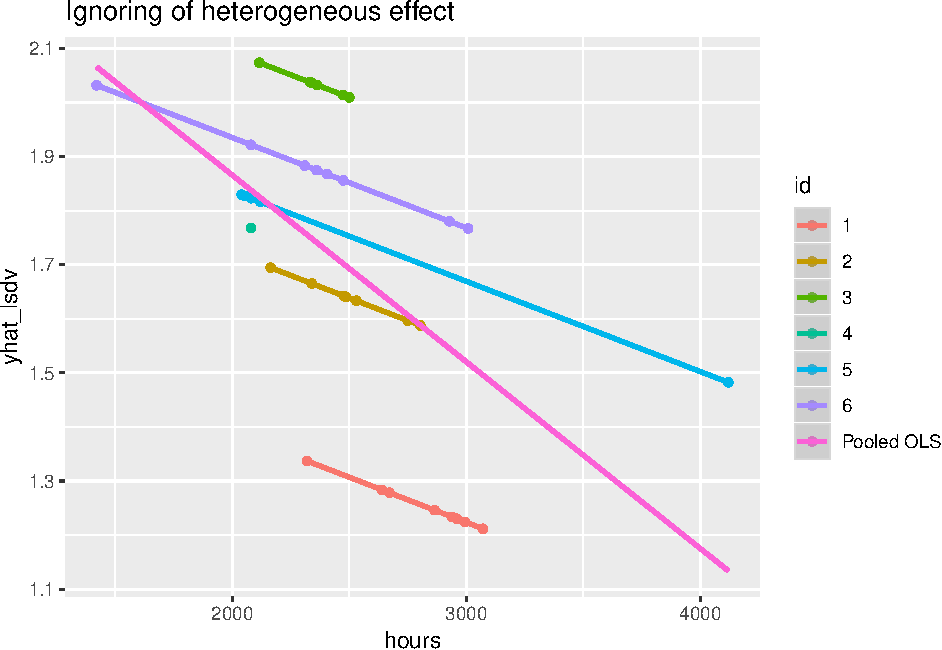
\includegraphics{09-paneldata_files/figure-latex/ignoring hetero-1.pdf}

Теперь то же самое в Stata

Для начала подгрузим данные и посмотрим на них. Сперва визуализируем малый датасет.

\begin{verbatim}
use lwage_panel_small
summarize
\end{verbatim}

\begin{verbatim}
    Variable |        Obs        Mean    Std. Dev.       Min        Max
-------------+---------------------------------------------------------
          nr |         48    364.6667    390.3276         13        910
        year |         48      1983.5    2.315535       1980       1987
       black |         48          .5    .5052912          0          1
       exper |         48    5.833333    2.636353          1         11
        hisp |         48           0           0          0          0
-------------+---------------------------------------------------------
       hours |         48    2407.875    425.1116       1420       4120
     married |         48       .1875    .3944428          0          1
        educ |         48          13     .825137         12         14
       union |         48        .125    .3342187          0          1
       lwage |         48    1.724878    .4719456  -.7202626   2.873161
-------------+---------------------------------------------------------
     expersq |         48    40.83333      31.933          1        121
  occupation |         48    4.083333    2.359529          1          9
          id |         48         3.5    1.725898          1          6
\end{verbatim}

\begin{verbatim}
xtset id year
xtline hours, overlay
clear
\end{verbatim}

\begin{verbatim}
       panel variable:  id (strongly balanced)
        time variable:  year, 1980 to 1987
                delta:  1 unit
\end{verbatim}

\begin{verbatim}
use lwage_panel_large
xtset id year
summarize
\end{verbatim}

\begin{verbatim}
       panel variable:  id (strongly balanced)
        time variable:  year, 1980 to 1987
                delta:  1 unit

    Variable |        Obs        Mean    Std. Dev.       Min        Max
-------------+---------------------------------------------------------
          nr |      4,360    5262.059     3496.15         13      12548
        year |      4,360      1983.5    2.291551       1980       1987
       black |      4,360    .1155963    .3197769          0          1
       exper |      4,360    6.514679    2.825873          0         18
        hisp |      4,360    .1559633    .3628622          0          1
-------------+---------------------------------------------------------
       hours |      4,360    2191.257    566.3523        120       4992
     married |      4,360    .4389908    .4963208          0          1
        educ |      4,360    11.76697    1.746181          3         16
       union |      4,360    .2440367    .4295639          0          1
       lwage |      4,360    1.649147    .5326094  -3.579079    4.05186
-------------+---------------------------------------------------------
     expersq |      4,360    50.42477    40.78199          0        324
  occupation |      4,360    4.988532    2.319978          1          9
          id |      4,360         273    157.3457          1        545
\end{verbatim}

Визуализируем данные. Если необходимо разнести линии на разные графики, следует убрать прараметр `overlay'.

Сгенерируем новую переменную и оценим модель с фиксированными эффектами. Последний аргумент произведёт оценку стандартных ошибок переменных в форме Хубера/Уайта

\begin{verbatim}

xtreg lwage hours, fe vce(robust)
\end{verbatim}

\begin{verbatim}
Fixed-effects (within) regression               Number of obs     =      4,360
Group variable: id                              Number of groups  =        545

R-sq:                                           Obs per group:
     within  = 0.0000                                         min =          8
     between = 0.0004                                         avg =        8.0
     overall = 0.0001                                         max =          8

                                                F(1,544)          =       0.00
corr(u_i, Xb)  = -0.0144                        Prob > F          =     0.9822

                                   (Std. Err. adjusted for 545 clusters in id)
------------------------------------------------------------------------------
             |               Robust
       lwage |      Coef.   Std. Err.      t    P>|t|     [95% Conf. Interval]
-------------+----------------------------------------------------------------
       hours |  -5.59e-07   .0000251    -0.02   0.982    -.0000498    .0000487
       _cons |   1.650371   .0549505    30.03   0.000      1.54243    1.758312
-------------+----------------------------------------------------------------
     sigma_u |  .39075125
     sigma_e |  .38728237
         rho |  .50445844   (fraction of variance due to u_i)
------------------------------------------------------------------------------
\end{verbatim}

Сделаем то же самое для модели со случайными эффектами.

\begin{verbatim}
xtreg lwage hours, re vce(robust)
\end{verbatim}

\begin{verbatim}
Random-effects GLS regression                   Number of obs     =      4,360
Group variable: id                              Number of groups  =        545

R-sq:                                           Obs per group:
     within  = 0.0000                                         min =          8
     between = 0.0004                                         avg =        8.0
     overall = 0.0001                                         max =          8

                                                Wald chi2(1)      =       0.00
corr(u_i, X)   = 0 (assumed)                    Prob > chi2       =     0.9510

                                   (Std. Err. adjusted for 545 clusters in id)
------------------------------------------------------------------------------
             |               Robust
       lwage |      Coef.   Std. Err.      z    P>|z|     [95% Conf. Interval]
-------------+----------------------------------------------------------------
       hours |   1.46e-06   .0000238     0.06   0.951    -.0000451    .0000481
       _cons |   1.645945   .0549594    29.95   0.000     1.538227    1.753664
-------------+----------------------------------------------------------------
     sigma_u |  .36626431
     sigma_e |  .38728237
         rho |   .4721295   (fraction of variance due to u_i)
------------------------------------------------------------------------------
\end{verbatim}

Тест Хаусмана.

\begin{verbatim}
xtreg lwage hours, re
estimates store b_re
xtreg lwage hours, fe
estimates store b_fe
hausman b_fe b_re, sigmamore
\end{verbatim}

\begin{verbatim}
Random-effects GLS regression                   Number of obs     =      4,360
Group variable: id                              Number of groups  =        545

R-sq:                                           Obs per group:
     within  = 0.0000                                         min =          8
     between = 0.0004                                         avg =        8.0
     overall = 0.0001                                         max =          8

                                                Wald chi2(1)      =       0.01
corr(u_i, X)   = 0 (assumed)                    Prob > chi2       =     0.9128

------------------------------------------------------------------------------
       lwage |      Coef.   Std. Err.      z    P>|z|     [95% Conf. Interval]
-------------+----------------------------------------------------------------
       hours |   1.46e-06   .0000133     0.11   0.913    -.0000247    .0000276
       _cons |   1.645945   .0337055    48.83   0.000     1.579884    1.712007
-------------+----------------------------------------------------------------
     sigma_u |  .36626431
     sigma_e |  .38728237
         rho |   .4721295   (fraction of variance due to u_i)
------------------------------------------------------------------------------



Fixed-effects (within) regression               Number of obs     =      4,360
Group variable: id                              Number of groups  =        545

R-sq:                                           Obs per group:
     within  = 0.0000                                         min =          8
     between = 0.0004                                         avg =        8.0
     overall = 0.0001                                         max =          8

                                                F(1,3814)         =       0.00
corr(u_i, Xb)  = -0.0144                        Prob > F          =     0.9682

------------------------------------------------------------------------------
       lwage |      Coef.   Std. Err.      t    P>|t|     [95% Conf. Interval]
-------------+----------------------------------------------------------------
       hours |  -5.59e-07    .000014    -0.04   0.968     -.000028    .0000269
       _cons |   1.650371   .0312611    52.79   0.000     1.589081    1.711661
-------------+----------------------------------------------------------------
     sigma_u |  .39075125
     sigma_e |  .38728237
         rho |  .50445844   (fraction of variance due to u_i)
------------------------------------------------------------------------------
F test that all u_i=0: F(544, 3814) = 8.14                   Prob > F = 0.0000

                 ---- Coefficients ----
             |      (b)          (B)            (b-B)     sqrt(diag(V_b-V_B))
             |      b_fe         b_re        Difference          S.E.
-------------+----------------------------------------------------------------
       hours |   -5.59e-07     1.46e-06       -2.02e-06        4.26e-06
------------------------------------------------------------------------------
                           b = consistent under Ho and Ha; obtained from xtreg
            B = inconsistent under Ha, efficient under Ho; obtained from xtreg

    Test:  Ho:  difference in coefficients not systematic

                  chi2(1) = (b-B)'[(V_b-V_B)^(-1)](b-B)
                          =        0.22
                Prob>chi2 =      0.6354
\end{verbatim}

Оценим FD-модель.

\begin{verbatim}
reg D.(lwage hours), vce(robust) nocon
\end{verbatim}

\begin{verbatim}
Linear regression                               Number of obs     =      3,815
                                                F(1, 3814)        =      93.15
                                                Prob > F          =     0.0000
                                                R-squared         =     0.0483
                                                Root MSE          =     .43793

------------------------------------------------------------------------------
             |               Robust
     D.lwage |      Coef.   Std. Err.      t    P>|t|     [95% Conf. Interval]
-------------+----------------------------------------------------------------
       hours |
         D1. |   -.000203    .000021    -9.65   0.000    -.0002443   -.0001618
------------------------------------------------------------------------------
\end{verbatim}

Аналогично оцениваем модель pooled OLS.

\begin{verbatim}
reg lwage hours, vce(robust)
\end{verbatim}

\begin{verbatim}
Linear regression                               Number of obs     =      4,360
                                                F(1, 4358)        =       0.27
                                                Prob > F          =     0.6059
                                                R-squared         =     0.0001
                                                Root MSE          =     .53264

------------------------------------------------------------------------------
             |               Robust
       lwage |      Coef.   Std. Err.      t    P>|t|     [95% Conf. Interval]
-------------+----------------------------------------------------------------
       hours |   9.36e-06   .0000181     0.52   0.606    -.0000262    .0000449
       _cons |   1.628646   .0415015    39.24   0.000     1.547282     1.71001
------------------------------------------------------------------------------
\end{verbatim}

Оценим LSDV-модель.

\begin{verbatim}
areg lwage hours, absorb(id)
\end{verbatim}

\begin{verbatim}
Linear regression, absorbing indicators         Number of obs     =      4,360
                                                F(   1,   3814)   =       0.00
                                                Prob > F          =     0.9682
                                                R-squared         =     0.5374
                                                Adj R-squared     =     0.4713
                                                Root MSE          =     0.3873

------------------------------------------------------------------------------
       lwage |      Coef.   Std. Err.      t    P>|t|     [95% Conf. Interval]
-------------+----------------------------------------------------------------
       hours |  -5.59e-07    .000014    -0.04   0.968     -.000028    .0000269
       _cons |   1.650371   .0312611    52.79   0.000     1.589081    1.711661
-------------+----------------------------------------------------------------
          id |      F(544, 3814) =      8.142   0.000         (545 categories)
\end{verbatim}

Повторим в Python.

\begin{Shaded}
\begin{Highlighting}[]
\ImportTok{import}\NormalTok{ numpy }\ImportTok{as}\NormalTok{ np}
\ImportTok{import}\NormalTok{ pandas }\ImportTok{as}\NormalTok{ pd}
\end{Highlighting}
\end{Shaded}

\begin{verbatim}
Error in py_call_impl(callable, dots$args, dots$keywords): ModuleNotFoundError: No module named 'pandas'

Detailed traceback: 
  File "<string>", line 1, in <module>
\end{verbatim}

Подгрузим данные и для обозначения панельных данных присвоим соответствующие индексы. Зададим соответствующие зависимые и независимые переменные, а также регрессионную формулу. Переменная ``Entity effects'' (Фиксированные эффекты) обязательна для включения для корректного распознавания панельных данных. Если её не включить, результат будет отличаться от R и STATA.

\begin{Shaded}
\begin{Highlighting}[]
\NormalTok{df }\OperatorTok{=}\NormalTok{ pd.read_csv(}\StringTok{"lwage_panel_large.csv"}\NormalTok{)}
\end{Highlighting}
\end{Shaded}

\begin{verbatim}
Error in py_call_impl(callable, dots$args, dots$keywords): NameError: name 'pd' is not defined

Detailed traceback: 
  File "<string>", line 1, in <module>
\end{verbatim}

\begin{Shaded}
\begin{Highlighting}[]
\NormalTok{df }\OperatorTok{=}\NormalTok{ df.set_index([}\StringTok{'id'}\NormalTok{, }\StringTok{'year'}\NormalTok{])}
\end{Highlighting}
\end{Shaded}

\begin{verbatim}
Error in py_call_impl(callable, dots$args, dots$keywords): NameError: name 'df' is not defined

Detailed traceback: 
  File "<string>", line 1, in <module>
\end{verbatim}

\begin{Shaded}
\begin{Highlighting}[]
\NormalTok{formula }\OperatorTok{=} \StringTok{'lwage ~ 1 + hours + EntityEffects'}
\NormalTok{dependent }\OperatorTok{=}\NormalTok{ df.lwage}
\end{Highlighting}
\end{Shaded}

\begin{verbatim}
Error in py_call_impl(callable, dots$args, dots$keywords): NameError: name 'df' is not defined

Detailed traceback: 
  File "<string>", line 1, in <module>
\end{verbatim}

\begin{Shaded}
\begin{Highlighting}[]
\NormalTok{regressors }\OperatorTok{=}\NormalTok{ df[[}\StringTok{'hours'}\NormalTok{]]}
\end{Highlighting}
\end{Shaded}

\begin{verbatim}
Error in py_call_impl(callable, dots$args, dots$keywords): NameError: name 'df' is not defined

Detailed traceback: 
  File "<string>", line 1, in <module>
\end{verbatim}

\begin{Shaded}
\begin{Highlighting}[]
\BuiltInTok{print}\NormalTok{(df.head())}
\end{Highlighting}
\end{Shaded}

\begin{verbatim}
Error in py_call_impl(callable, dots$args, dots$keywords): NameError: name 'df' is not defined

Detailed traceback: 
  File "<string>", line 1, in <module>
\end{verbatim}

Оценим FE-модель, используя within-оценку.

\begin{Shaded}
\begin{Highlighting}[]
\ImportTok{from}\NormalTok{ linearmodels }\ImportTok{import}\NormalTok{ PanelOLS}
\end{Highlighting}
\end{Shaded}

\begin{verbatim}
Error in py_call_impl(callable, dots$args, dots$keywords): ModuleNotFoundError: No module named 'linearmodels'

Detailed traceback: 
  File "<string>", line 1, in <module>
\end{verbatim}

\begin{Shaded}
\begin{Highlighting}[]
\NormalTok{model_fe }\OperatorTok{=}\NormalTok{ PanelOLS.from_formula(formula, df)}
\end{Highlighting}
\end{Shaded}

\begin{verbatim}
Error in py_call_impl(callable, dots$args, dots$keywords): NameError: name 'PanelOLS' is not defined

Detailed traceback: 
  File "<string>", line 1, in <module>
\end{verbatim}

\begin{Shaded}
\begin{Highlighting}[]
\NormalTok{model_fe_fitted }\OperatorTok{=}\NormalTok{ model_fe.fit(cov_type}\OperatorTok{=}\StringTok{'clustered'}\NormalTok{, cluster_entity }\OperatorTok{=} \VariableTok{True}\NormalTok{)}
\end{Highlighting}
\end{Shaded}

\begin{verbatim}
Error in py_call_impl(callable, dots$args, dots$keywords): NameError: name 'model_fe' is not defined

Detailed traceback: 
  File "<string>", line 1, in <module>
\end{verbatim}

\begin{Shaded}
\begin{Highlighting}[]
\BuiltInTok{print}\NormalTok{(model_fe_fitted)}
\end{Highlighting}
\end{Shaded}

\begin{verbatim}
Error in py_call_impl(callable, dots$args, dots$keywords): NameError: name 'model_fe_fitted' is not defined

Detailed traceback: 
  File "<string>", line 1, in <module>
\end{verbatim}

Оценим RE-модель, используя FGLS-оценку.

\begin{Shaded}
\begin{Highlighting}[]
\ImportTok{from}\NormalTok{ linearmodels.panel }\ImportTok{import}\NormalTok{ RandomEffects}
\end{Highlighting}
\end{Shaded}

\begin{verbatim}
Error in py_call_impl(callable, dots$args, dots$keywords): ModuleNotFoundError: No module named 'linearmodels'

Detailed traceback: 
  File "<string>", line 1, in <module>
\end{verbatim}

\begin{Shaded}
\begin{Highlighting}[]
\NormalTok{model_re }\OperatorTok{=}\NormalTok{ RandomEffects.from_formula(formula, df)}
\end{Highlighting}
\end{Shaded}

\begin{verbatim}
Error in py_call_impl(callable, dots$args, dots$keywords): NameError: name 'RandomEffects' is not defined

Detailed traceback: 
  File "<string>", line 1, in <module>
\end{verbatim}

\begin{Shaded}
\begin{Highlighting}[]
\NormalTok{model_re_fitted }\OperatorTok{=}\NormalTok{ model_re.fit(cov_type}\OperatorTok{=}\StringTok{'clustered'}\NormalTok{, cluster_entity }\OperatorTok{=} \VariableTok{True}\NormalTok{)}
\end{Highlighting}
\end{Shaded}

\begin{verbatim}
Error in py_call_impl(callable, dots$args, dots$keywords): NameError: name 'model_re' is not defined

Detailed traceback: 
  File "<string>", line 1, in <module>
\end{verbatim}

\begin{Shaded}
\begin{Highlighting}[]
\BuiltInTok{dir}\NormalTok{(model_re_fitted)}
\end{Highlighting}
\end{Shaded}

\begin{verbatim}
Error in py_call_impl(callable, dots$args, dots$keywords): NameError: name 'model_re_fitted' is not defined

Detailed traceback: 
  File "<string>", line 1, in <module>
\end{verbatim}

\begin{Shaded}
\begin{Highlighting}[]
\BuiltInTok{print}\NormalTok{(model_re_fitted)}
\end{Highlighting}
\end{Shaded}

\begin{verbatim}
Error in py_call_impl(callable, dots$args, dots$keywords): NameError: name 'model_re_fitted' is not defined

Detailed traceback: 
  File "<string>", line 1, in <module>
\end{verbatim}

Тест Хаусмана в соответствующем пакете на данный момент не реализован.

Оценим модель Pooled OLS

\begin{Shaded}
\begin{Highlighting}[]
\ImportTok{from}\NormalTok{ linearmodels.panel }\ImportTok{import}\NormalTok{ PooledOLS}
\end{Highlighting}
\end{Shaded}

\begin{verbatim}
Error in py_call_impl(callable, dots$args, dots$keywords): ModuleNotFoundError: No module named 'linearmodels'

Detailed traceback: 
  File "<string>", line 1, in <module>
\end{verbatim}

\begin{Shaded}
\begin{Highlighting}[]
\NormalTok{model_pool }\OperatorTok{=}\NormalTok{ PooledOLS.from_formula(formula, df)}
\end{Highlighting}
\end{Shaded}

\begin{verbatim}
Error in py_call_impl(callable, dots$args, dots$keywords): NameError: name 'PooledOLS' is not defined

Detailed traceback: 
  File "<string>", line 1, in <module>
\end{verbatim}

\begin{Shaded}
\begin{Highlighting}[]
\NormalTok{model_pool_fitted }\OperatorTok{=}\NormalTok{ model_pool.fit(cov_type}\OperatorTok{=}\StringTok{'clustered'}\NormalTok{, cluster_entity }\OperatorTok{=} \VariableTok{True}\NormalTok{)}
\end{Highlighting}
\end{Shaded}

\begin{verbatim}
Error in py_call_impl(callable, dots$args, dots$keywords): NameError: name 'model_pool' is not defined

Detailed traceback: 
  File "<string>", line 1, in <module>
\end{verbatim}

\begin{Shaded}
\begin{Highlighting}[]
\BuiltInTok{print}\NormalTok{(model_pool_fitted)}
\end{Highlighting}
\end{Shaded}

\begin{verbatim}
Error in py_call_impl(callable, dots$args, dots$keywords): NameError: name 'model_pool_fitted' is not defined

Detailed traceback: 
  File "<string>", line 1, in <module>
\end{verbatim}

Оценим LSDV-модель

\begin{Shaded}
\begin{Highlighting}[]
\NormalTok{model_lsdv }\OperatorTok{=}\NormalTok{ PanelOLS.from_formula(formula, df)}
\NormalTok{model_lsdv_fitted }\OperatorTok{=}\NormalTok{ model_lsdv.fit(cov_type}\OperatorTok{=}\StringTok{'clustered'}\NormalTok{, cluster_entity }\OperatorTok{=} \VariableTok{True}\NormalTok{, use_lsdv }\OperatorTok{=} \VariableTok{True}\NormalTok{)}
\BuiltInTok{print}\NormalTok{(model_lsdv_fitted)}
\end{Highlighting}
\end{Shaded}

Построим FD-оценку. Здесь необходимо убрать константный признак, так как данная модель начинает выдавать ошибку. Логически, конечно, он автоматически должен исчезнуть по построению модели, но в данной реализации это требуется задать на уровне пользователя.

\begin{Shaded}
\begin{Highlighting}[]
\ImportTok{from}\NormalTok{ linearmodels.panel }\ImportTok{import}\NormalTok{ FirstDifferenceOLS}
\end{Highlighting}
\end{Shaded}

\begin{verbatim}
Error in py_call_impl(callable, dots$args, dots$keywords): ModuleNotFoundError: No module named 'linearmodels'

Detailed traceback: 
  File "<string>", line 1, in <module>
\end{verbatim}

\begin{Shaded}
\begin{Highlighting}[]
\NormalTok{formula_fd }\OperatorTok{=} \StringTok{'lwage ~ hours + EntityEffects'}
\NormalTok{model_fd }\OperatorTok{=}\NormalTok{ FirstDifferenceOLS.from_formula(formula_fd, df)}
\end{Highlighting}
\end{Shaded}

\begin{verbatim}
Error in py_call_impl(callable, dots$args, dots$keywords): NameError: name 'FirstDifferenceOLS' is not defined

Detailed traceback: 
  File "<string>", line 1, in <module>
\end{verbatim}

\begin{Shaded}
\begin{Highlighting}[]
\NormalTok{model_fd_fitted }\OperatorTok{=}\NormalTok{ model_fd.fit(cov_type}\OperatorTok{=}\StringTok{'clustered'}\NormalTok{, cluster_entity }\OperatorTok{=} \VariableTok{True}\NormalTok{)}
\end{Highlighting}
\end{Shaded}

\begin{verbatim}
Error in py_call_impl(callable, dots$args, dots$keywords): NameError: name 'model_fd' is not defined

Detailed traceback: 
  File "<string>", line 1, in <module>
\end{verbatim}

\begin{Shaded}
\begin{Highlighting}[]
\BuiltInTok{print}\NormalTok{(model_fd_fitted)}
\end{Highlighting}
\end{Shaded}

\begin{verbatim}
Error in py_call_impl(callable, dots$args, dots$keywords): NameError: name 'model_fd_fitted' is not defined

Detailed traceback: 
  File "<string>", line 1, in <module>
\end{verbatim}

\hypertarget{heterosked}{%
\chapter{Гетероскедастичность в простой регрессии}\label{heterosked}}

\hypertarget{pca}{%
\chapter{PCA}\label{pca}}

\hypertarget{dinpanel}{%
\chapter{Динамические панели}\label{dinpanel}}

\hypertarget{tobit_heckit}{%
\chapter{TOBIT, HECKIT}\label{tobit_heckit}}

\begin{Shaded}
\begin{Highlighting}[]
\KeywordTok{library}\NormalTok{(ggplot2)}
\KeywordTok{library}\NormalTok{(AER) }\CommentTok{#tobit}
\KeywordTok{library}\NormalTok{(sampleSelection) }\CommentTok{#heckit}
\end{Highlighting}
\end{Shaded}

\begin{verbatim}
Error in library(sampleSelection): there is no package called 'sampleSelection'
\end{verbatim}

\begin{Shaded}
\begin{Highlighting}[]
\KeywordTok{library}\NormalTok{(}\StringTok{'ltm'}\NormalTok{) }\CommentTok{#margins}
\end{Highlighting}
\end{Shaded}

\begin{verbatim}
Error in library("ltm"): there is no package called 'ltm'
\end{verbatim}

\begin{Shaded}
\begin{Highlighting}[]
\KeywordTok{library}\NormalTok{(}\StringTok{'foreign'}\NormalTok{)}
\KeywordTok{library}\NormalTok{(skimr)}
\end{Highlighting}
\end{Shaded}

Данная глава посвящена моделям с цензурированными выборками. В таких выборках часть значений целевой переменной будет дискретной переменной, а часть - непрерывной. Простой пример, который указывается в некоторых учебниках, это исследование расходов семей на автомобили. Каждая семья может либо потратить какую-то сумму на автомобиль, либо, если она не может позволить себе автомобиль, то значение расходов будет равно нулю. Соответственно, переменная демонстрирует либо факт неучастия в покупке автомобиля, либо степень участия в виде суммы. Оценивается в данном случае обычная регрессионная модель, но с функцией правдоподобия следующего вида:

\begin{equation}
L=\prod_{y_{t}=0}\left(1-\Phi\left(\frac{\boldsymbol{x}_{t}^{\prime} \boldsymbol{\beta}}{\sigma}\right)\right) \prod_{y_{t}>0} \frac{1}{\sqrt{2 \pi} \sigma} \exp \left(-\frac{1}{2 \sigma^{2}}\left(y_{t}-\boldsymbol{x}_{t}^{\prime} \boldsymbol{\beta}\right)^{2}\right)
\end{equation}

Для начала подгрузим данные и визуализируем их. Этот датасет результаты тестирования двухсот школьников по шкале от 200 до 800 (apt), а также их успеваемость по чтению и математике (read и math соответственно). Построим гистограмму, наложив поверх неё функцию плотности нормального распределения.

\begin{Shaded}
\begin{Highlighting}[]
\NormalTok{data =}\StringTok{ }\KeywordTok{read.csv}\NormalTok{(}\StringTok{'tobit.csv'}\NormalTok{)}
\end{Highlighting}
\end{Shaded}

\begin{Shaded}
\begin{Highlighting}[]
\CommentTok{# Функция, генерирующая функцию плотности нормального распределения в соответствии с распределением вектора входных данных}
\NormalTok{f <-}\StringTok{ }\ControlFlowTok{function}\NormalTok{(x, var, }\DataTypeTok{bw =} \DecValTok{15}\NormalTok{) \{}
  \KeywordTok{dnorm}\NormalTok{(x, }\DataTypeTok{mean =} \KeywordTok{mean}\NormalTok{(var), }\KeywordTok{sd}\NormalTok{(var)) }\OperatorTok{*}\StringTok{ }\KeywordTok{length}\NormalTok{(var)  }\OperatorTok{*}\StringTok{ }\NormalTok{bw}
\NormalTok{\}}


\NormalTok{p <-}\StringTok{ }\KeywordTok{ggplot}\NormalTok{(data, }\KeywordTok{aes}\NormalTok{(}\DataTypeTok{x =}\NormalTok{ apt, }\DataTypeTok{fill=}\NormalTok{prog))}
\NormalTok{p }\OperatorTok{+}\StringTok{ }\KeywordTok{stat_bin}\NormalTok{(}\DataTypeTok{binwidth=}\DecValTok{15}\NormalTok{) }\OperatorTok{+}
\StringTok{  }\KeywordTok{stat_function}\NormalTok{(}\DataTypeTok{fun =}\NormalTok{ f, }\DataTypeTok{size =} \DecValTok{1}\NormalTok{,}
    \DataTypeTok{args =} \KeywordTok{list}\NormalTok{(}\DataTypeTok{var =}\NormalTok{ data}\OperatorTok{$}\NormalTok{apt))}
\end{Highlighting}
\end{Shaded}

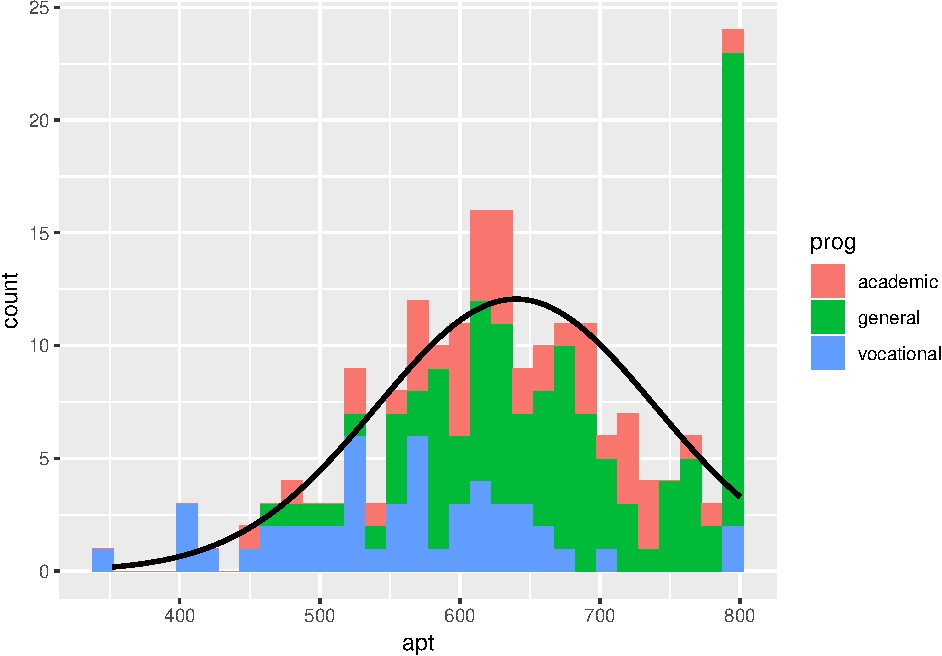
\includegraphics{13-tobit_heckit_files/figure-latex/hist plot chunk-1.pdf}

Как можем видеть, нашлось довольно много школьников, которые написали тест на высший балл. В связи с этим распределение даллеко от нормального из-за ограничений баллов теста. Вид выборки также довольно специфичен при взгляде на диаграмму рассеяния. Довольно различимая линейная зависимость как бы сплюснута сверху.

\begin{Shaded}
\begin{Highlighting}[]
\NormalTok{g <-}\StringTok{ }\KeywordTok{ggplot}\NormalTok{(data, }\KeywordTok{aes}\NormalTok{(math, apt, }\DataTypeTok{col =}\NormalTok{ prog))}
\NormalTok{g }\OperatorTok{+}\KeywordTok{geom_point}\NormalTok{()}
\end{Highlighting}
\end{Shaded}

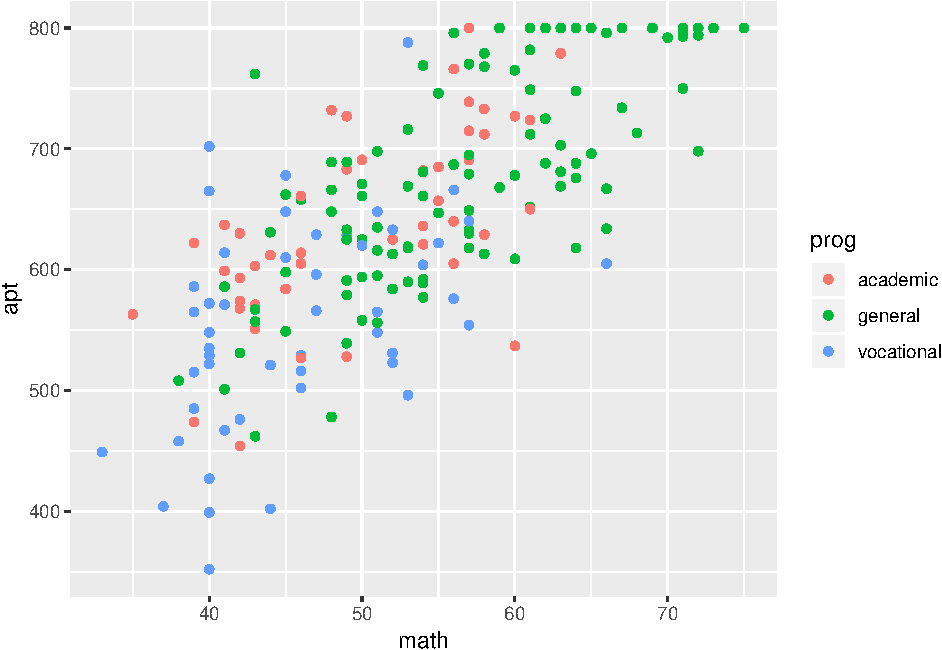
\includegraphics{13-tobit_heckit_files/figure-latex/scatter plot chunk-1.pdf}

Оценим Тобит-модель:

\begin{Shaded}
\begin{Highlighting}[]
\NormalTok{model_tobit =}\StringTok{ }\KeywordTok{tobit}\NormalTok{(apt }\OperatorTok{~}\StringTok{ }\NormalTok{math }\OperatorTok{+}\StringTok{ }\NormalTok{read, }\DataTypeTok{data =}\NormalTok{ data, }\DataTypeTok{right =} \DecValTok{800}\NormalTok{)}
\KeywordTok{summary}\NormalTok{(model_tobit)}
\end{Highlighting}
\end{Shaded}

\begin{verbatim}

Call:
tobit(formula = apt ~ math + read, right = 800, data = data)

Observations:
         Total  Left-censored     Uncensored Right-censored 
           200              0            183             17 

Coefficients:
             Estimate Std. Error z value Pr(>|z|)    
(Intercept) 159.00366   29.90374   5.317 1.05e-07 ***
math          6.34441    0.70306   9.024  < 2e-16 ***
read          2.88961    0.63295   4.565 4.99e-06 ***
Log(scale)    4.21923    0.05293  79.719  < 2e-16 ***
---
Signif. codes:  0 '***' 0.001 '**' 0.01 '*' 0.05 '.' 0.1 ' ' 1

Scale: 67.98 

Gaussian distribution
Number of Newton-Raphson Iterations: 5 
Log-likelihood: -1047 on 4 Df
Wald-statistic: 266.2 on 2 Df, p-value: < 2.22e-16 
\end{verbatim}

Модель Тобина имеет ряд ограничений. Основное из них -- это зависимость вероятности участия и интенсивности участия определяется одним и тем же набором переменных. Для преодоления этих ограничений была предложена модель Хекмана. В ней принятие решения ``участвовать - не участвовать'' и определение степени участия могут зависеть от разных переменных.

Загрузим другие данные во славу разнообразия.

\begin{Shaded}
\begin{Highlighting}[]
\NormalTok{data =}\StringTok{ }\KeywordTok{read.dta}\NormalTok{(}\StringTok{'data_alcohol&tobacco.dta'}\NormalTok{)}
\KeywordTok{summary}\NormalTok{(data)}
\end{Highlighting}
\end{Shaded}

\begin{verbatim}
     obs                 age           bluecol            lnx       
 Length:2724        Min.   :0.000   Min.   :0.0000   Min.   :11.76  
 Class :character   1st Qu.:1.000   1st Qu.:0.0000   1st Qu.:13.41  
 Mode  :character   Median :2.000   Median :0.0000   Median :13.76  
                    Mean   :2.408   Mean   :0.1468   Mean   :13.73  
                    3rd Qu.:4.000   3rd Qu.:0.0000   3rd Qu.:14.06  
                    Max.   :4.000   Max.   :1.0000   Max.   :15.33  
    flanders         nadults        ninfants           nkids       
 Min.   :0.0000   Min.   :1.00   Min.   :0.00000   Min.   :0.0000  
 1st Qu.:0.0000   1st Qu.:1.00   1st Qu.:0.00000   1st Qu.:0.0000  
 Median :0.0000   Median :2.00   Median :0.00000   Median :0.0000  
 Mean   :0.4519   Mean   :1.97   Mean   :0.04479   Mean   :0.5646  
 3rd Qu.:1.0000   3rd Qu.:2.00   3rd Qu.:0.00000   3rd Qu.:1.0000  
 Max.   :1.0000   Max.   :7.00   Max.   :2.00000   Max.   :5.0000  
     resid                shalc              shtob        
 Min.   :-0.9797682   Min.   :0.000000   Min.   :0.00000  
 1st Qu.: 0.0626030   1st Qu.:0.002906   1st Qu.:0.00000  
 Median : 0.1223031   Median :0.010898   Median :0.00000  
 Mean   : 0.0001171   Mean   :0.017828   Mean   :0.01224  
 3rd Qu.: 0.1854353   3rd Qu.:0.024244   3rd Qu.:0.01381  
 Max.   : 0.5795787   Max.   :0.211124   Max.   :0.19276  
    walloon          whitecol      shalc_tobit             alc        
 Min.   :0.0000   Min.   :0.000   Min.   :-0.005627   Min.   :0.0000  
 1st Qu.:0.0000   1st Qu.:0.000   1st Qu.: 0.010925   1st Qu.:1.0000  
 Median :0.0000   Median :0.000   Median : 0.015169   Median :1.0000  
 Mean   :0.3814   Mean   :0.333   Mean   : 0.015198   Mean   :0.8289  
 3rd Qu.:1.0000   3rd Qu.:1.000   3rd Qu.: 0.019735   3rd Qu.:1.0000  
 Max.   :1.0000   Max.   :1.000   Max.   : 0.032814   Max.   :1.0000  
      tob        
 Min.   :0.0000  
 1st Qu.:0.0000  
 Median :0.0000  
 Mean   :0.3803  
 3rd Qu.:1.0000  
 Max.   :1.0000  
\end{verbatim}

\begin{Shaded}
\begin{Highlighting}[]
\NormalTok{f <-}\StringTok{ }\ControlFlowTok{function}\NormalTok{(x, var, }\DataTypeTok{bw =} \DecValTok{15}\NormalTok{) \{}
  \KeywordTok{dnorm}\NormalTok{(x, }\DataTypeTok{mean =} \KeywordTok{mean}\NormalTok{(var), }\KeywordTok{sd}\NormalTok{(var)) }\OperatorTok{*}\StringTok{ }\KeywordTok{length}\NormalTok{(var)  }\OperatorTok{*}\StringTok{ }\NormalTok{bw}
\NormalTok{\}}


\NormalTok{p <-}\StringTok{ }\KeywordTok{ggplot}\NormalTok{(data, }\KeywordTok{aes}\NormalTok{(}\DataTypeTok{x =}\NormalTok{ shalc))}
\NormalTok{p }\OperatorTok{+}\StringTok{ }\KeywordTok{stat_bin}\NormalTok{(}\DataTypeTok{binwidth=}\FloatTok{0.01}\NormalTok{) }\OperatorTok{+}
\StringTok{  }\KeywordTok{stat_function}\NormalTok{(}\DataTypeTok{fun =}\NormalTok{ f, }\DataTypeTok{size =} \DecValTok{1}\NormalTok{,}
    \DataTypeTok{args =} \KeywordTok{list}\NormalTok{(}\DataTypeTok{var =}\NormalTok{ data}\OperatorTok{$}\NormalTok{alc))}
\end{Highlighting}
\end{Shaded}

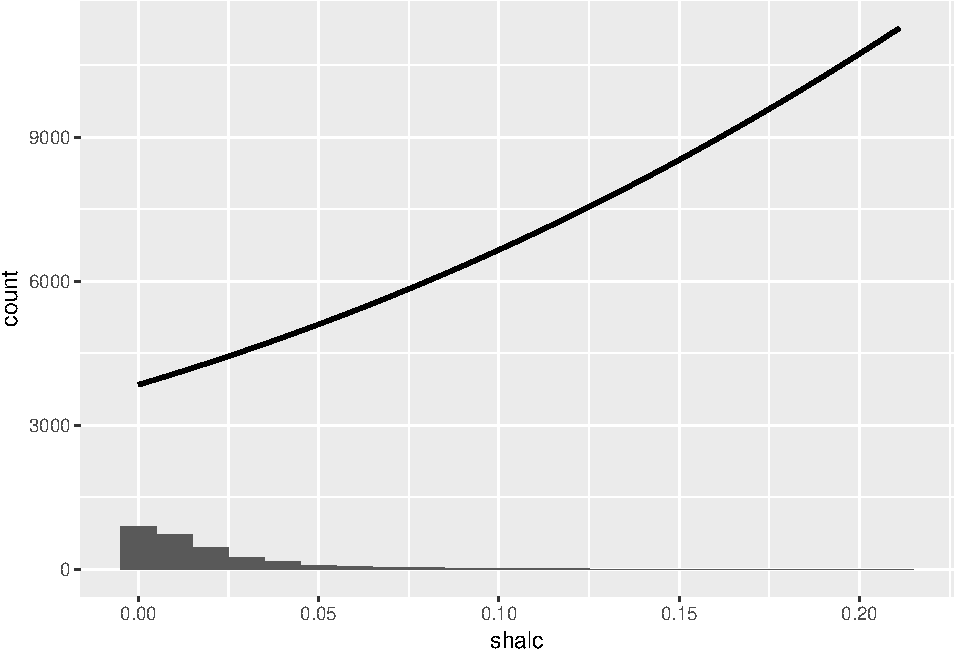
\includegraphics{13-tobit_heckit_files/figure-latex/unnamed-chunk-2-1.pdf}

\begin{Shaded}
\begin{Highlighting}[]
\NormalTok{heck1 =}\StringTok{ }\KeywordTok{heckit}\NormalTok{(alc }\OperatorTok{~}\StringTok{ }\NormalTok{age }\OperatorTok{+}\StringTok{ }\NormalTok{nadults }\OperatorTok{+}\StringTok{ }\NormalTok{nkids }\OperatorTok{+}\StringTok{ }\NormalTok{lnx }\OperatorTok{+}\StringTok{ }\NormalTok{walloon, shalc }\OperatorTok{~}\StringTok{  }\NormalTok{age }\OperatorTok{+}\StringTok{ }\NormalTok{nadults }\OperatorTok{+}\StringTok{ }\NormalTok{nkids }\OperatorTok{+}\StringTok{ }\NormalTok{lnx }\OperatorTok{+}\StringTok{ }\NormalTok{walloon, }\DataTypeTok{data =}\NormalTok{ data, }\DataTypeTok{method =} \StringTok{'ml'}\NormalTok{)}
\end{Highlighting}
\end{Shaded}

\begin{verbatim}
Error in heckit(alc ~ age + nadults + nkids + lnx + walloon, shalc ~ age + : could not find function "heckit"
\end{verbatim}

\begin{Shaded}
\begin{Highlighting}[]
\KeywordTok{summary}\NormalTok{(heck1)}
\end{Highlighting}
\end{Shaded}

\begin{verbatim}
Error in summary(heck1): object 'heck1' not found
\end{verbatim}

\begin{Shaded}
\begin{Highlighting}[]
\NormalTok{heck2 =}\StringTok{ }\KeywordTok{heckit2fit}\NormalTok{(alc }\OperatorTok{~}\StringTok{ }\NormalTok{age }\OperatorTok{+}\StringTok{ }\NormalTok{nadults }\OperatorTok{+}\StringTok{ }\NormalTok{nkids }\OperatorTok{+}\StringTok{ }\NormalTok{lnx }\OperatorTok{+}\StringTok{ }\NormalTok{walloon, shalc }\OperatorTok{~}\StringTok{  }\NormalTok{age }\OperatorTok{+}\StringTok{ }\NormalTok{nadults }\OperatorTok{+}\StringTok{ }\NormalTok{nkids }\OperatorTok{+}\StringTok{ }\NormalTok{lnx }\OperatorTok{+}\StringTok{ }\NormalTok{walloon, }\DataTypeTok{data =}\NormalTok{ data)}
\end{Highlighting}
\end{Shaded}

\begin{verbatim}
Error in heckit2fit(alc ~ age + nadults + nkids + lnx + walloon, shalc ~ : could not find function "heckit2fit"
\end{verbatim}

\begin{Shaded}
\begin{Highlighting}[]
\KeywordTok{summary}\NormalTok{(heck2)}
\end{Highlighting}
\end{Shaded}

\begin{verbatim}
Error in summary(heck2): object 'heck2' not found
\end{verbatim}

Теперь то же самое в STATA.

\begin{verbatim}
clear
use tobit
summarize
\end{verbatim}

\begin{verbatim}
    Variable |        Obs        Mean    Std. Dev.       Min        Max
-------------+---------------------------------------------------------
          v1 |        200        99.5    57.87918          0        199
    unnamed0 |        200        99.5    57.87918          0        199
          id |        200       100.5    57.87918          1        200
        read |        200       52.23    10.25294         28         76
        math |        200      52.645    9.368448         33         75
-------------+---------------------------------------------------------
        prog |          0
         apt |        200     640.035    99.21903        352        800
         top |        200        .915    .2795815          0          1
\end{verbatim}

\begin{verbatim}
egen prog_2 = group(prog)
tobit apt read math i.prog_2, ul
\end{verbatim}

\begin{verbatim}
Tobit regression                                Number of obs     =        200
                                                LR chi2(4)        =     188.97
                                                Prob > chi2       =     0.0000
Log likelihood = -1041.0629                     Pseudo R2         =     0.0832

------------------------------------------------------------------------------
         apt |      Coef.   Std. Err.      t    P>|t|     [95% Conf. Interval]
-------------+----------------------------------------------------------------
        read |   2.697939    .618798     4.36   0.000     1.477582    3.918296
        math |   5.914485   .7098063     8.33   0.000     4.514647    7.314323
             |
      prog_2 |
          2  |  -12.71476   12.40629    -1.02   0.307    -37.18173     11.7522
          3  |   -46.1439   13.72401    -3.36   0.001     -73.2096   -19.07821
             |
       _cons |    209.566   32.77154     6.39   0.000     144.9359    274.1961
-------------+----------------------------------------------------------------
      /sigma |   65.67672   3.481272                      58.81116    72.54228
------------------------------------------------------------------------------
             0  left-censored observations
           183     uncensored observations
            17 right-censored observations at apt >= 800
\end{verbatim}

\begin{verbatim}
clear all
use data_alcohol&tobacco
heckman shalc age nadults nkids lnx walloon, select(alc = age nadults nkids lnx walloon)
\end{verbatim}

\begin{verbatim}
Iteration 0:   log likelihood =  4309.5307  
Iteration 1:   log likelihood =  4311.3949  
Iteration 2:   log likelihood =  4311.4638  
Iteration 3:   log likelihood =  4311.4649  
Iteration 4:   log likelihood =  4311.4649  

Heckman selection model                         Number of obs     =      2,724
(regression model with sample selection)        Censored obs      =        466
                                                Uncensored obs    =      2,258

                                                Wald chi2(5)      =     126.74
Log likelihood =  4311.465                      Prob > chi2       =     0.0000

------------------------------------------------------------------------------
             |      Coef.   Std. Err.      z    P>|z|     [95% Conf. Interval]
-------------+----------------------------------------------------------------
shalc        |
         age |   .0022075   .0003854     5.73   0.000     .0014521     .002963
     nadults |  -.0017463   .0006455    -2.71   0.007    -.0030114   -.0004812
       nkids |  -.0021381    .000564    -3.79   0.000    -.0032435   -.0010327
         lnx |   -.001557   .0014823    -1.05   0.294    -.0044622    .0013483
     walloon |   .0025647   .0009575     2.68   0.007     .0006881    .0044413
       _cons |   .0413301   .0205898     2.01   0.045     .0009749    .0816853
-------------+----------------------------------------------------------------
alc          |
         age |    .064492   .0233269     2.76   0.006     .0187722    .1102118
     nadults |  -.0865676   .0419754    -2.06   0.039    -.1688379   -.0042973
       nkids |  -.0847672   .0362055    -2.34   0.019    -.1557287   -.0138058
         lnx |   .8839885   .0758532    11.65   0.000      .735319    1.032658
     walloon |   .1975137    .062286     3.17   0.002     .0754353    .3195921
       _cons |  -11.12847   .9982321   -11.15   0.000    -13.08497   -9.171975
-------------+----------------------------------------------------------------
     /athrho |  -.0062433   .1345632    -0.05   0.963    -.2699823    .2574956
    /lnsigma |  -3.841538   .0148838  -258.10   0.000    -3.870709   -3.812366
-------------+----------------------------------------------------------------
         rho |  -.0062433   .1345579                     -.2636083    .2519516
       sigma |   .0214606   .0003194                      .0208436    .0220958
      lambda |   -.000134   .0028877                     -.0057938    .0055259
------------------------------------------------------------------------------
LR test of indep. eqns. (rho = 0):   chi2(1) =     0.00   Prob > chi2 = 0.9640
\end{verbatim}

\begin{verbatim}
heckman shalc age nadults nkids lnx walloon, select(alc = age nadults nkids lnx walloon) twostep
\end{verbatim}

\begin{verbatim}
> nx walloon) twostep

Heckman selection model -- two-step estimates   Number of obs     =      2,724
(regression model with sample selection)        Censored obs      =        466
                                                Uncensored obs    =      2,258

                                                Wald chi2(5)      =     125.15
                                                Prob > chi2       =     0.0000

------------------------------------------------------------------------------
             |      Coef.   Std. Err.      z    P>|z|     [95% Conf. Interval]
-------------+----------------------------------------------------------------
shalc        |
         age |    .002117   .0005482     3.86   0.000     .0010426    .0031915
     nadults |  -.0016402    .000792    -2.07   0.038    -.0031925   -.0000879
       nkids |  -.0020387   .0007089    -2.88   0.004    -.0034282   -.0006492
         lnx |  -.0027209   .0052148    -0.52   0.602    -.0129417    .0074998
     walloon |   .0023175   .0014319     1.62   0.106    -.0004889     .005124
       _cons |   .0584579   .0763935     0.77   0.444    -.0912706    .2081865
-------------+----------------------------------------------------------------
alc          |
         age |    .064482   .0233247     2.76   0.006     .0187665    .1101975
     nadults |  -.0865298   .0419629    -2.06   0.039    -.1687756   -.0042839
       nkids |  -.0847535   .0362048    -2.34   0.019    -.1557135   -.0137934
         lnx |   .8839584   .0758491    11.65   0.000     .7352969     1.03262
     walloon |   .1974812   .0622813     3.17   0.002     .0754121    .3195503
       _cons |   -11.1281   .9981866   -11.15   0.000    -13.08451   -9.171695
-------------+----------------------------------------------------------------
mills        |
      lambda |   -.003805    .016022    -0.24   0.812    -.0352075    .0275975
-------------+----------------------------------------------------------------
         rho |   -0.17633
       sigma |  .02157888
------------------------------------------------------------------------------
\end{verbatim}

\hypertarget{treatment}{%
\chapter{Treatment effect}\label{treatment}}

\hypertarget{compatability}{%
\chapter{Что-то там про совместимость и языки}\label{compatability}}

\hypertarget{dict}{%
\chapter{Словарь}\label{dict}}

\bibliography{book.bib,packages.bib}


\end{document}
